% !TEX program = xelatex
\documentclass[UTF8,fontset=fandol,a4paper,11pt]{ctexart}
\usepackage[margin=21mm,top=23mm,bottom=22mm,headheight=16pt]{geometry}
\usepackage{amsmath,amssymb,mathtools,bm}
\usepackage{tikz}
\usetikzlibrary{arrows.meta,calc,angles,quotes,patterns,decorations.pathmorphing}
\usepackage{xcolor,booktabs,array,longtable,enumitem,fancyhdr,needspace}
\usepackage[unicode,hidelinks]{hyperref}
\definecolor{ink}{HTML}{24343C}
\definecolor{accent}{HTML}{166A70}
\definecolor{muted}{HTML}{65747A}
\definecolor{rulegray}{HTML}{D4DDE0}
\definecolor{warm}{HTML}{966037}
\color{ink}
\setlength{\parindent}{2em}
\setlength{\parskip}{4pt}
\linespread{1.12}
\AtBeginDocument{\setlength{\abovedisplayskip}{6pt plus 2pt minus 1pt}
\setlength{\belowdisplayskip}{6pt plus 2pt minus 1pt}
\setlength{\abovedisplayshortskip}{0pt plus 1pt}
\setlength{\belowdisplayshortskip}{4pt plus 1pt}}
\setlist[enumerate]{label=(\arabic*),leftmargin=2.3em,itemsep=3pt,topsep=4pt}
\setlist[itemize]{leftmargin=2em,itemsep=2pt,topsep=4pt}
\allowdisplaybreaks[1]
\setlength{\emergencystretch}{2em}
\setcounter{secnumdepth}{0}
\providecommand{\tightlist}{\setlength{\itemsep}{0pt}\setlength{\parskip}{0pt}}
\ctexset{section={format=\Large\bfseries\color{accent},beforeskip=10pt,afterskip=9pt},
subsection={format=\normalsize\bfseries\color{accent},beforeskip=10pt,afterskip=4pt},
subsubsection={format=\normalsize\bfseries,beforeskip=8pt,afterskip=3pt}}
\pagestyle{fancy}
\fancyhf{}
\fancyhead[L]{\small\color{muted}物理学难题集萃}
% 页眉仅保留书名；版本名称只在封面显示。
\fancyfoot[L]{\small\color{muted}\chapterlabel}
\fancyfoot[R]{\small\thepage}
\renewcommand{\headrulewidth}{0.4pt}
\renewcommand{\footrulewidth}{0pt}
\newcommand{\dd}{\mathop{}\!\mathrm{d}}
\newcommand{\vect}[1]{\bm{#1}}
\newcommand{\tagline}[1]{\noindent{\small\color{muted}#1}\par}
\newcommand{\result}[1]{\begin{equation*}\boxed{#1}\end{equation*}}
\newcommand{\figcaption}[1]{\par\vspace{2pt}{\small\color{muted}#1}\par}
\newcommand{\teach}[2]{\Needspace{4\baselineskip}\subsection*{讲解要点与追问}#1\par\smallskip\noindent\textbf{追问：}#2\par}
\newcommand{\workarea}{\par\vspace{7mm}\noindent{\small\color{muted}作答区}\par\vspace{4mm}
\noindent\textcolor{rulegray}{\rule{\linewidth}{0.3pt}}\par\vspace{16mm}
\noindent\textcolor{rulegray}{\rule{\linewidth}{0.3pt}}\par\vspace{16mm}
\noindent\textcolor{rulegray}{\rule{\linewidth}{0.3pt}}\par\vspace{16mm}
\noindent\textcolor{rulegray}{\rule{\linewidth}{0.3pt}}}
\tikzset{axis/.style={-{Stealth[length=2mm]},thin,color=muted},
motion/.style={-{Stealth[length=2.3mm]},thick,color=accent},
force/.style={-{Stealth[length=2.3mm]},thick,color=warm},
traj/.style={thick,color=accent},guide/.style={dashed,thin,color=muted},
object/.style={thick,color=ink},every node/.style={font=\small}}\widowpenalty=10000\clubpenalty=10000\displaywidowpenalty=10000\newcommand{\chapterlabel}{电磁学第五章\quad 交流电路、暂态过程及其他}





\newcommand{\shortworkarea}{\par\vspace{7mm}\noindent{\small\color{muted}作答区}\par\vspace{4mm}
\noindent\textcolor{rulegray}{\rule{\linewidth}{0.3pt}}\par\vspace{16mm}
\noindent\textcolor{rulegray}{\rule{\linewidth}{0.3pt}}\par\vspace{16mm}
\noindent\textcolor{rulegray}{\rule{\linewidth}{0.3pt}}}


\hypersetup{pdftitle={电磁学第五章 交流电路、暂态过程及其他·学生解答版},pdfauthor={}}

\begin{document}\pdfbookmark[0]{电磁学第五章 交流电路、暂态过程及其他}{cover}

\thispagestyle{empty}\vspace*{22mm}
\noindent{\Huge\bfseries 物理学难题集萃}\par\vspace{10mm}
\noindent{\LARGE 电磁学第五章}\par\vspace{6mm}
\noindent{\LARGE 交流电路、暂态过程及其他}\par\vspace{12mm}
\noindent{\Large\color{accent}学生解答版}\par\vspace{9mm}
\noindent\textcolor{accent}{\rule{\linewidth}{1pt}}\par\vspace{9mm}
\noindent 第1--20题\par\vfill\clearpage
\pdfbookmark[1]{题目目录}{contents}\section*{题目目录}
\begin{longtable}{@{}r p{113mm} r@{}}\toprule 题号 & 题目 & 页码\\\midrule

\hyperref[q:1]{1} & \hyperref[q:1]{偏轴旋转线圈的电流、力矩与能量} & \pageref{q:1} \\

\hyperref[q:2]{2} & \hyperref[q:2]{随时间变化的门限与张弛振荡} & \pageref{q:2} \\

\hyperref[q:3]{3} & \hyperref[q:3]{一次闪亮后不再点燃的氖灯} & \pageref{q:3} \\

\hyperref[q:4]{4} & \hyperref[q:4]{任意波形下保持平衡的电感电桥} & \pageref{q:4} \\

\hyperref[q:5]{5} & \hyperref[q:5]{三元件黑盒的连接与参数识别} & \pageref{q:5} \\

\hyperref[q:6]{6} & \hyperref[q:6]{不对称星形负载与中性点漂移} & \pageref{q:6} \\

\hyperref[q:7]{7} & \hyperref[q:7]{非正弦电源的谐波叠加与瞬时投影} & \pageref{q:7} \\

\hyperref[q:8]{8} & \hyperref[q:8]{含电抗桥支路的复阻抗网络} & \pageref{q:8} \\

\hyperref[q:9]{9} & \hyperref[q:9]{有损线圈的等效模型与导纳电桥} & \pageref{q:9} \\

\hyperref[q:10]{10} & \hyperref[q:10]{交流跳环的相位与平均斥力} & \pageref{q:10} \\

\hyperref[q:11]{11} & \hyperref[q:11]{并联谐振的带宽、自由振荡与持久环流} & \pageref{q:11} \\

\hyperref[q:12]{12} & \hyperref[q:12]{无限电感电容链的色散与传播速度} & \pageref{q:12} \\

\hyperref[q:13]{13} & \hyperref[q:13]{完全互感耦合回路的充放电与快慢模式} & \pageref{q:13} \\

\hyperref[q:14]{14} & \hyperref[q:14]{双电容电阻网的两个衰减模式} & \pageref{q:14} \\

\hyperref[q:15]{15} & \hyperref[q:15]{带电容反馈的阶跃放大器} & \pageref{q:15} \\

\hyperref[q:16]{16} & \hyperref[q:16]{漏电电容分压与不交换的极限} & \pageref{q:16} \\

\hyperref[q:17]{17} & \hyperref[q:17]{正弦电源接通时的电容充电暂态} & \pageref{q:17} \\

\hyperref[q:18]{18} & \hyperref[q:18]{大气电场、离子中和与旋转电场仪} & \pageref{q:18} \\

\hyperref[q:19]{19} & \hyperref[q:19]{假设磁单极子的线圈探测} & \pageref{q:19} \\

\hyperref[q:20]{20} & \hyperref[q:20]{切连科夫辐射的几何、阈值与测量误差} & \pageref{q:20} \\

\bottomrule\end{longtable}

电压采用有向差$U_{AB}=V_A-V_B$，电流按图示箭头取正。正弦量以题设说明区分峰值与有效值；同频复相量采用余弦约定。换路问题保留初始储能，稳态结论只用于已进入相应周期状态的过程。

\clearpage

\pdfbookmark[2]{第 1 题 偏轴旋转线圈的电流、力矩与能量}{q1}

\section*{第 1 题\quad 偏轴旋转线圈的电流、力矩与能量}\label{q:1}


矩形闭合线圈有$N$匝，竖直边长$l$，水平边长$3b$，电阻为$R$、自感为$L$。线圈在水平匀强磁场$B_0$中绕竖直轴转动，转轴距两条竖直边分别为$b$和$2b$。角速度为$\omega$，$t=0$时线圈平面与磁场平行。
\begin{enumerate}
\item 证明：一个微小时间内，维持转动的外力所做的功等于感应电动势向电路提供的电能。
\item 写出电流$i$的方程。$\omega$为正常量时，代入$i=I_0\cos(\omega t+\varphi)$，求$I_0$及$\varphi$，并说明该式描述的状态。
\item 求稳态下每转一周电阻消耗的能量及理想电感净吸收的能量。
\end{enumerate}

\begin{center}\begin{minipage}{.98\linewidth}\centering
\begin{tikzpicture}[scale=.95,transform shape]

\draw[object] (-2,0)--(2,1)--(2,4)--(-2,3)--cycle;
\draw[object] (-1.9,.08)--(2.1,1.08)--(2.1,4.08)--(-1.9,3.08)--cycle;
\draw[axis] (-.667,-.7)--(-.667,4.8) node[above]{转轴};
\foreach \y in {.5,1.5,2.5,3.5}{\draw[motion] (3,\y)--(4.3,\y);}
\node at (4,4.1){$\vect B_0$};\node[left] at (-2,1.5){$l$};
\draw[guide] (-2,3.5)--(-.667,3.83)--(2,4.5);
\node[fill=white] at (-1.4,3.8){$b$};\node[fill=white] at (.8,4.45){$2b$};
\node at (.5,-1.05){$N\text{匝},R,L$};

\end{tikzpicture}
\figcaption{图电5.1\quad 偏轴线圈；水平总边长为$3b$}
\end{minipage}\end{center}

\Needspace{6\baselineskip}\subsection*{解答}


取图电5.1中的有向转角$\theta$为线圈平面与$\vect B_0$的夹角，沿解图电5.1B的回路取电流正向，使发电电动势在$\theta=0$时为正。所选有向磁通为$-3blB_0\sin\theta$。

\begin{center}\begin{minipage}{.97\linewidth}\centering
\begin{tikzpicture}[scale=.95,transform shape]
\begin{scope}
\draw[axis] (-2,0)--(3,0);\draw[object] (-1.15,-.69)--(2.3,1.38);
\fill (0,0) circle(.045);\node[below right] at (0,0){$O$};
\draw[motion] (1.8,-1.2)--(3,-1.2) node[right]{$\vect B_0$};
\draw[force] (-1.15,-.69)--(-1.15,.6) node[left]{$F$};
\draw[force] (2.3,1.38)--(2.3,.08) node[right]{$F$};
\node[below left] at (-1.15,-.69){$\odot\, i$};\node[above right] at (2.3,1.38){$\otimes\, i$};
\draw[guide] (-1.15,-.69)--(-1.15,-1.5) (2.3,1.38)--(2.3,-1.5);
\draw[<->] (-1.15,-1.5)--(0,-1.5) node[midway,below]{$b\cos\theta$};
\draw[<->] (0,-1.5)--(2.3,-1.5) node[midway,below]{$2b\cos\theta$};
\draw (0.7,0) arc(0:31:.7);\node at (1,.25){$\theta$};
\node at (.4,2.25){俯视与力臂};
\end{scope}
\end{tikzpicture}
\figcaption{解图电5.1A　俯视的两条竖边及安培力；图示取$i>0$。平衡它们的外力反向，力臂之和为$3b\cos\theta$。}
\end{minipage}\end{center}


在解图电5.1A所示的$i>0$时，两条竖直边的安培力大小均为$F=Ni lB_0$；若电流为负，两箭头反向，力的大小为$N|i|lB_0$。解图电5.1A的俯视图中，它们对转轴的力臂分别为$b\cos\theta$和$2b\cos\theta$。外力平衡磁力矩时，
\[
 M_{\rm ext}=3Ni b lB_0\cos\theta,\qquad
 \dd W_{\rm ext}=3Ni b lB_0\cos\theta\,\dd\theta .
\]
同一正向下，法拉第定律给出
\[
 \mathcal E=-N\frac{\dd\Phi}{\dd t}
 =3Nb lB_0\dot\theta\cos\theta .
\]
因而$\dd W_{\rm ext}=\mathcal E i\,\dd t$。瞬时功率也可出现$\mathcal E i<0$：某些时段电路把储存的磁场能送回机械系统，外力此时需要制动。

\begin{center}\begin{minipage}{.97\linewidth}\centering
\begin{tikzpicture}[scale=.95,transform shape]
\begin{scope}[shift={(5.0,1.0)},rotate=90.0]\draw[object] (-1.0,0)--(-0.33,0) (0.33,0)--(1.0,0);\draw[object,fill=white] (0,0) circle (.33);\draw[object] plot[domain=-.23:.23,samples=35] (\x,{.12*sin(780*\x)});\end{scope}\node[anchor=east,fill=white,inner sep=1.5pt] at (4.6600,1.0000) {$\mathcal E$};
\begin{scope}[shift={(6.5,2.0)},rotate=0.0]\draw[object] (-1.5,0)--(-0.48,0) (0.48,0)--(1.5,0);\draw[object,decorate,decoration={coil,aspect=.45,segment length=4pt,amplitude=3pt}] (-.48,0)--(.48,0);\end{scope}\node[anchor=south,fill=white,inner sep=1.5pt] at (6.5000,2.3400) {$L$};
\begin{scope}[shift={(8.0,1.0)},rotate=-90.0]\draw[object] (-1.0,0)--(-0.48,0) (0.48,0)--(1.0,0);\draw[object,fill=white] (-.48,-.14) rectangle (.48,.14);\end{scope}\node[anchor=west,fill=white,inner sep=1.5pt] at (8.3400,1.0000) {$R$};
\draw[object] (8,0)--(5,0);
\draw[motion] (6.8,-.3)--(5.7,-.3) node[midway,below]{$i$};
\node at (6.5,2.8){等效回路};

\end{tikzpicture}
\figcaption{解图电5.1B　动生电动势、自感与电阻组成同一闭合回路。正电流方向决定有向磁通和回路方程的符号。}
\end{minipage}\end{center}

解图电5.1B的等效回路满足$L\dot i+Ri=\mathcal E(t)$。恒定$\omega>0$时，$\theta=\omega t$，记$\mathcal E_0=3Nb lB_0\omega$。代入试探式，按$\cos\omega t$和$\sin\omega t$比较系数：
\[
 I_0(R\cos\varphi-\omega L\sin\varphi)=\mathcal E_0,\quad
 I_0(R\sin\varphi+\omega L\cos\varphi)=0.
\]
由于$R>0$，取$-\pi/2<\varphi<0$，有
\[
 \boxed{I_0=\frac{\mathcal E_0}{\sqrt{R^2+\omega^2L^2}},\qquad
 \varphi=-\arctan\frac{\omega L}{R}.}
\]
用相量图可把两项的合成写成一个带相位的余弦。记$Z=\sqrt{R^2+\omega^2L^2}$，选$0<\alpha<\pi/2$使
\[
\cos\alpha=R/Z,\quad \sin\alpha=\omega L/Z,\quad \tan\alpha=\omega L/R.
\]
则试探式代入回路后右侧可写成
\[
RI_0\cos(\omega t+\varphi)-\omega LI_0\sin(\omega t+\varphi)
=I_0Z\cos(\omega t+\varphi+\alpha).
\]
与$\mathcal E_0\cos\omega t$比较，振幅要求$I_0Z=\mathcal E_0$，相位要求$\varphi+\alpha=0$，仍得上述负相位。辅助角三角形正对应解图电5.1C，其中 $\underline{\mathcal E}$ 在 $\underline I$ 的前方。

这是周期稳态。若初始电流$i(0)=i_s$，完整解还含衰减项：
\[
 i(t)=I_0\cos(\omega t+\varphi)
 +(i_s-I_0\cos\varphi)e^{-Rt/L}.
\]
只有指数项已经衰减，或初始电流恰与稳态相符时，电流才只有余弦项。\begin{center}\begin{minipage}{.97\linewidth}\centering
\begin{tikzpicture}[scale=.95,transform shape]
\begin{scope}[shift={(10.2,0)}]
\draw[axis] (-.2,0)--(3,0);\draw[axis] (0,-.2)--(0,2.2);
\draw[motion] (0,0)--(2.3,0) node[below]{$\underline U_R$};
\draw[force] (2.3,0)--(2.3,1.6) node[right]{$\underline U_L$};
\draw[traj,-{Stealth}] (0,0)--(2.3,1.6) node[midway,above left]{$\underline{\mathcal E}$};
\node[below] at (1,-.3){$\underline I\parallel\underline U_R$};
\node at (1.3,2.8){稳态相量};
\end{scope}

\end{tikzpicture}
\figcaption{解图电5.1C　周期稳态的电压相量。电流与电阻电压同相，电感电压超前90度，感应电动势为两者的矢量和。}
\end{minipage}\end{center}

解图电5.1C中$\underline U_R$与$\underline I$同向，$\underline U_L$超前$\underline I$四分之一周期，两者之和是$\underline{\mathcal E}$。

稳态一周$T=2\pi/\omega$内，
\begin{align*}
 W_R&=R I_0^2\int_{t_0}^{t_0+T}\cos^2(\omega t+\varphi)\,\dd t\\
 &=\frac{\pi R\mathcal E_0^2}{\omega(R^2+\omega^2L^2)}
 =\boxed{\frac{9\pi N^2b^2l^2B_0^2R\omega}{R^2+\omega^2L^2}}.
\end{align*}
理想电感的瞬时功率为$Li\dot i$，积分是储能改变量：
\[
 W_L=\left[\frac12Li^2\right]_{t_0}^{t_0+T}=0.
\]
电感一周内交替储能、放能，净吸收为零；外力一周净做功为$W_R$。若从开机时刻计一周，则用开机与首周末的实际电流求 $W_L$。


上述微元功只指外力平衡安培力矩的部分。若还改变转速，总机械功另须计入转动动能变化；本题稳态比较保持角速度恒定。回路式乘以i，逐时刻的能量关系为
\[
P_{\rm ext}=\mathcal E i=Ri^2+\frac{\dd}{\dd t}\left(\frac12Li^2\right).
\]
所以“机械功转为电能”既包括焦耳热，也包括电感储能增加；维持匀速的外力既可驱动，也可制动。
\begin{center}\begin{minipage}{.97\linewidth}\centering
\begin{tikzpicture}[scale=.78,transform shape,font=\small]
\draw[axis](0,-1.1)--(0,4)node[above]{功率$/(\mathcal E_0^2/R)$};\draw[axis](0,0)--(7.1,0)node[right]{$s=\omega t$};
\draw[blue,thick,domain=0:6.283185,samples=150]plot(\x,{5*cos(deg(\x))*(cos(deg(\x))+sin(deg(\x))-exp(-\x))/2});
\draw[orange!80!black,thick,domain=0:6.283185,samples=150]plot(\x,{5*((cos(deg(\x))+sin(deg(\x))-exp(-\x))/2)^2});
\draw[guide](3.141593,-.2)--(3.141593,3.5) (6.283185,-.2)--(6.283185,3.5);
\node[below]at(3.141593,-.25){$\pi$};\node[below]at(6.283185,-.25){$2\pi$};\node[left]at(0,2.5){$1/2$};
\node[align=left,anchor=west]at(7.6,2){示意取$\omega L=R,\ i(0)=0$\\蓝线：$P_{\rm ext}=\mathcal E i$\\橙线：$P_R=Ri^2$\\两线之差为磁场储能变化率\\蓝线可短时为负，橙线恒非负};
\end{tikzpicture}
\figcaption{解图电5.1D　初始无电流时的首周功率示例。两条曲线的竖直差是电感功率，首、末的储能差由实际电流给出。}
\end{minipage}\end{center}

解图电5.1D所画的电流为$i=(\mathcal E_0/R)f(s)$，$f(s)=[\cos s+\sin s-e^{-s}]/2$。它在s=0确为零，随后才接近稳态余弦。蓝线为$(\mathcal E_0^2/R)f(s)\cos s$，橙线为$(\mathcal E_0^2/R)f^2(s)$；蓝线下降到橙线下方时，电感在释放已储磁能。

例如初始$i_s=0$、从$t=0$起计一周，令$\rho=e^{-RT/L}$，则$i(T)=I_0\cos\varphi(1-\rho)$，该周电感净吸收
\[
\Delta W_L=\frac12LI_0^2\cos^2\varphi(1-\rho)^2>0.
\]
在解图电5.1D中，机械功是首周蓝线下的代数面积，焦耳热是橙线下的面积；两面积之差等于上述 $\Delta W_L$。若始末都在同一周期稳态，图C的相量解给出相同的首尾电流，此差为零。


\Needspace{13\baselineskip}

\pdfbookmark[2]{第 2 题 随时间变化的门限与张弛振荡}{q2}

\section*{第 2 题\quad 随时间变化的门限与张弛振荡}\label{q:2}


恒流源$S$输出$I_0>0$，给电容$C$充电。电子开关$K$与$C$并联，由信号$u_F(t)=U_1+U_0\sin\omega t$控制，其中$U_1>U_0>0$。$u_F$只控制开关，不向电容充放电。当$u_C$首次达到当时的$u_F$时，$K$闭合，使$u_C$近乎竖直降至$U_{\min}$后立即断开；$0<U_{\min}<U_1-U_0$。
\begin{enumerate}
\item 在同一$u$--$t$图画$u_F$、$U_{\min}$和$u_C$。初始$U_{\min}\le u_C(0)<u_F(0)$。
\item 若某组参数和触发初相使相邻触发时刻的间隔始终相同，求触发时的电压，并检查等间隔条件的全部可能分支。
\end{enumerate}

\begin{center}\begin{minipage}{.98\linewidth}\centering
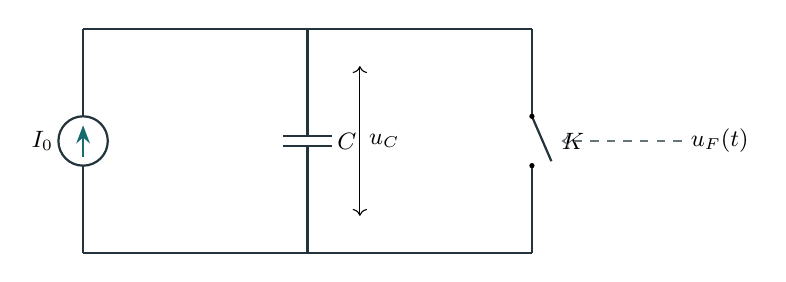
\begin{tikzpicture}[scale=.95,transform shape]
\begin{scope}[shift={(0.0,1.5)},rotate=90.0]\draw[object] (-1.5,0)--(-0.33,0) (0.33,0)--(1.5,0);\draw[object,fill=white] (0,0) circle (.33);\draw[motion] (-.21,0)--(.21,0);\end{scope}\node[anchor=east,fill=white,inner sep=1.5pt] at (-0.3400,1.5000) {$I_0$};
\draw[object] (0,3)--(6,3);
\draw[object] (0,0)--(6,0);
\begin{scope}[shift={(3.0,1.5)},rotate=-90.0]\draw[object] (-1.5,0)--(-0.22,0) (0.22,0)--(1.5,0);\draw[object] (-.07,-.33)--(-.07,.33) (.07,-.33)--(.07,.33) (-.22,0)--(-.07,0) (.07,0)--(.22,0);\end{scope}\node[anchor=west,fill=white,inner sep=1.5pt] at (3.3400,1.5000) {$C$};
\begin{scope}[shift={(6.0,1.5)},rotate=-90.0]\draw[object] (-1.5,0)--(-0.33,0) (0.33,0)--(1.5,0);\draw[object] (-.33,0)--(.27,.26);\fill (-.33,0) circle (.035) (.33,0) circle (.035);\end{scope}\node[anchor=west,fill=white,inner sep=1.5pt] at (6.3400,1.5000) {$K$};
\draw[guide,->] (8,1.5)--(6.4,1.5);\node[right] at (8,1.5){$u_F(t)$};
\draw[<->] (3.7,.5)--(3.7,2.5) node[midway,right]{$u_C$};
\end{tikzpicture}
\figcaption{图电5.2\quad 恒流充电与受门限控制的并联复位开关}
\end{minipage}\end{center}

\Needspace{6\baselineskip}\subsection*{解答}


图电5.2的虚线只表示控制关系，恒流源、电容和开关才构成实际充放电通路。门限的高低并不改变开关断开时的充电斜率；开关一旦触发，就以题设的极短复位过程把电压带回同一个低值。下面忽略这段复位用时，保留每一段实际首次相遇。

记$a=I_0/C$。图电5.2中开关断开时，电流全流入电容，故$\dot u_C=a$。第一段为$u_C(0)+at$；解图电5.2A的斜线均有斜率$a$，上端是与门限的首次交点，竖直复位后落在$U_{\min}$。

\begin{center}\begin{minipage}{.97\linewidth}\centering
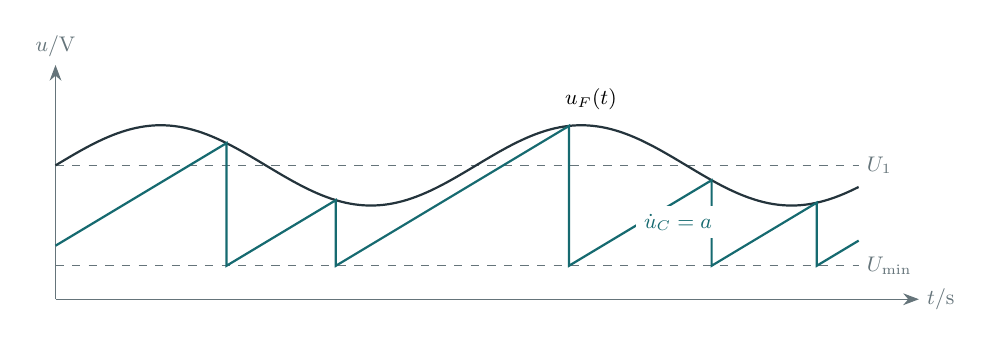
\begin{tikzpicture}[scale=.85,transform shape]
\draw[axis](0,0)--(12.9,0)node[right]{$t/\mathrm s$};\draw[axis](0,0)--(0,3.5)node[above]{$u/\mathrm V$};
\draw[guide](0,.5)--(12,.5)node[right]{$U_{\min}$};\draw[guide](0,2)--(12,2)node[right]{$U_1$};
\draw[object,domain=0:12,samples=170]plot(\x,{2+.6*sin(deg(\x))});\node[above]at(8,2.7){$u_F(t)$};
\draw[traj]plot coordinates {(0.00000000,0.80000000) (2.55419595,2.33251757) (2.55419595,0.50000000) (4.18837715,1.48050872) (4.18837715,0.50000000) (7.67183410,2.59007417) (7.67183410,0.50000000) (9.80277472,1.77856437) (9.80277472,0.50000000) (11.37325074,1.44228561) (11.37325074,0.50000000) (12.00000000,0.87604956)};\node[text=accent,fill=white]at(9.3,1.15){$\dot u_C=a$};
\end{tikzpicture}
\figcaption{解图电5.2A　实际首次交点与瞬间复位。示例取$U_1=2\,\mathrm V,U_0=0.6\,\mathrm V,U_{\min}=0.5\,\mathrm V,a=0.6\,\mathrm{V/s},\omega=1\,\mathrm s^{-1},u_C(0)=0.8\,\mathrm V$。}
\end{minipage}\end{center}


设触发时刻为$t_n$。忽略复位用时，
\[
 u_C(t)=U_{\min}+a(t-t_n),\quad t_n<t<t_{n+1},
\]
\[
 U_{\min}+a(t_{n+1}-t_n)=U_1+U_0\sin\omega t_{n+1}.
\]
若所有间隔为$\Delta>0$，每次触发电压相同：
\[
 U_*=U_{\min}+a\Delta,\quad
 \sin(\alpha+n\delta)=s,\quad\delta=\omega\Delta,\quad
 s=\frac{U_*-U_1}{U_0}.
\]
对连续三个相位用$s_{n+1}+s_{n-1}=2s_n\cos\delta$，得$s(1-\cos\delta)=0$，非零 $s$ 要求 $\cos\delta=1$；$s=0$ 时，触发相位可在两个零点间交替。

第一支为$\delta=2k\pi$，$k=1,2,\ldots$，即整数个门限周期触发一次：
\[
 \boxed{\Delta=\frac{2k\pi}{\omega},\quad
 U_*=U_{\min}+\frac{2k\pi I_0}{C\omega}.}
\]
以下以$\tau$表示复位后经过的时间。候选电压必须位于$[U_1-U_0,U_1+U_0]$，并且存在某个触发相位$\alpha$，使
\[
 U_{\min}+a\tau<U_1+U_0\sin(\alpha+\omega\tau),\qquad0<\tau<\Delta.
\]
这里$\alpha$为上一次复位的相位。等式定终点；不等式保证充电线到终点才遇到门限。

第二支$s=0$，各次都在$U_1$触发，相位是正弦零点。除已包含在第一支的偶数倍$\pi$外，还可能有
\[
 \boxed{U_*=U_1,\quad\Delta=\frac{m\pi}{\omega},\quad
 \frac{I_0}{C\omega}=\frac{d}{m\pi}},\qquad
 m=1,3,5,\ldots,\quad d=U_1-U_{\min}.
\]
两种零点交替。到达上升零点前，门限减斜线约为$[d/(m\pi)-U_0]\varepsilon$，所以需$d\ge m\pi U_0$。它也是充分条件：对$0<x<m\pi$，
\[
 d\left(1-\frac{x}{m\pi}\right)\pm U_0\sin x
 \ge \frac d{m\pi}(m\pi-x)-U_0|\sin x|>0,
\]
利用$|\sin x|\le m\pi-x$，内点仍无提前交点。这支要求$d\ge m\pi U_0$及上述斜率匹配。

解图电5.2B画出$m=1$的可行轨迹，每半周期在$U_1$触发一次。这里讨论的是已进入等间隔序列的状态，任意初值的第一段未必已经锁定。

\begin{center}\begin{minipage}{.97\linewidth}\centering
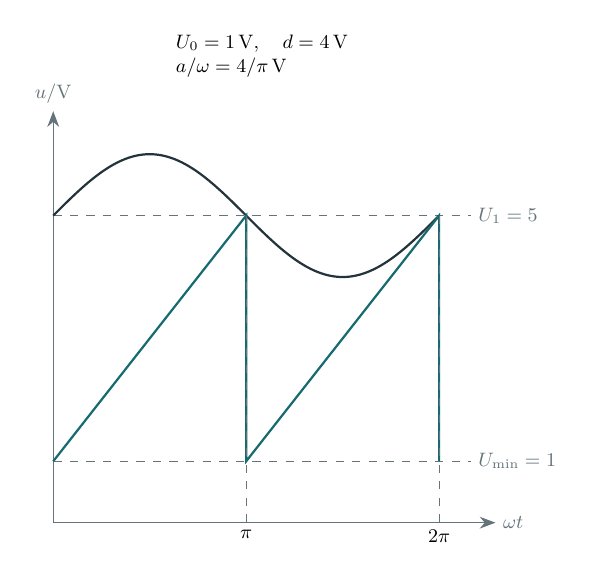
\begin{tikzpicture}[scale=.78,transform shape]
\draw[axis](0,0)--(7.2,0)node[right]{$\omega t$};\draw[axis](0,0)--(0,6.7)node[above]{$u/\mathrm V$};
\draw[guide](0,1)--(6.8,1)node[right]{$U_{\min}=1$};\draw[guide](0,5)--(6.8,5)node[right]{$U_1=5$};
\draw[object,domain=0:6.283185,samples=130]plot(\x,{5+sin(deg(\x))});
\draw[traj](0,1)--(3.141593,5)--(3.141593,1)--(6.283185,5)--(6.283185,1);
\draw[guide](3.141593,0)--(3.141593,5) (6.283185,0)--(6.283185,5);
\node[below]at(3.141593,0){$\pi$};\node[below]at(6.283185,0){$2\pi$};
\node[align=left]at(3.4,7.6){$U_0=1\,\mathrm V,\quad d=4\,\mathrm V$\\$a/\omega=4/\pi\,\mathrm V$};
\end{tikzpicture}
\figcaption{解图电5.2B　$m=1$时的半周期交替触发。每次端点电压相同，但正弦零点方向交替；此图数值与A图分别表示两组参数。}
\end{minipage}\end{center}



解图电5.2A中，第一次斜段从给定初压出发，之后每次才从$U_{\min}$重新起步。端点必须既满足相等，又是此前区间的第一个相等位置。A图有五次触发，虽然充电线平行，门限高低不同，各段等待时间也不同。复位到低门限后，任意一段的持续时间必有
\[
\frac{d-U_0}{a}\le t_{n+1}-t_n\le\frac{d+U_0}{a},\qquad d=U_1-U_{\min}>U_0.
\]
这是由上门限始终位于$[U_1-U_0,U_1+U_0]$和固定充电斜率得到的有限正区间；对于有给定初压的第一段，将两端界限中的 $U_{\min}$ 换成 $u_C(0)$，并取实际的第一个相遇时刻。

相位分类也可逐步看清：若共同正弦值$s\ne0$，递推关系迫使$\cos\delta=1$，只有整周期一支。若$s=0$，$\alpha$和$\alpha+\delta$都为整数倍$\pi$，故$\delta=m\pi$；偶数m已经属于前一支，正奇数m才给B图式的零点交替。两个端点相同电压并不要求它们具有同一相位。
\begin{center}\begin{minipage}{.97\linewidth}\centering
\begin{tikzpicture}[scale=.95,transform shape,font=\small]
\draw[axis](0,-.65)--(0,4.6)node[above]{$G_h(x)$};\draw[axis](0,0)--(3.7,0)node[right]{$x$};
\draw[blue,thick,domain=0:3.141593,samples=120]plot(\x,{4*(1-\x/pi)-sin(deg(\x))});
\draw[orange!80!black,thick,domain=0:3.141593,samples=120]plot(\x,{pi*(1-\x/pi)-sin(deg(\x))});
\draw[muted,dashed,thick,domain=0:3.141593,samples=120]plot(\x,{2*(1-\x/pi)-sin(deg(\x))});
\fill[muted](1.570796,0)circle(1.6pt);\node[below]at(1.570796,-.1){$\pi/2$};\node[below]at(3.141593,-.1){$\pi$};
\node[align=left,anchor=west]at(4.2,2.7){$G_h=h(1-x/\pi)-\sin x$\\蓝线$h=4$：内点始终为正\\橙线$h=\pi$：到终点才为零\\灰线$h=2$：$\pi/2$提前触发\\候选终点$\pi$已不是首次交点};
\end{tikzpicture}
\figcaption{解图电5.2C　半周期内门限与充电线的电压差。纵轴是下降半周期内“上门限减充电直线”除以$U_0$，$h=d/U_0$；灰线的提前零点使候选失效。}
\end{minipage}\end{center}

解图电5.2C选取从下降零点复位到下一上升零点的半周期，$x=\omega(t-t_n)$。两曲线电压差正是$U_0G_h(x)$。灰线h=2虽在$x=\pi$也回到零，却在$x=\pi/2$已经相遇，开关会在那里复位，后面的候选轨迹不再属于实际过程。蓝线h=4对应B图，严格先保持正差，终点才触发。

临界h等于$\pi$时，令$r=\pi-x$，有$G_\pi=r-\sin r>0$，所有内点仍未触发；接近终点时差为$r^3/6+O(r^5)$。这里两线终点斜率相同，但以三阶项穿越，按“达到即触发”的规则仍成立。一般正奇数m同样令$r=m\pi-x$，用$|\sin x|=|\sin r|<r$补足严格首次条件，得到$d\ge m\pi U_0$。

整数周期支中，若 $a\ge\omega U_0$，门限 $H(t)=U_1+U_0\sin\omega t$ 减充电线的导数 $H'(t)-a$ 处处非正，且除孤立点外为负。相位与候选触发电压匹配时，电压差就在端点首次降到零。若 $a<\omega U_0$，用前面的全区间不等式寻找首次交点。

再看解图电5.2B两个交点的斜率。设一次触发的时间偏离等间隔轨迹 $\delta t_n$，下一次偏离 $\delta t_{n+1}$。对 $H(t_{n+1})-U_{\min}=a(t_{n+1}-t_n)$ 求一阶变化：
\[
\bigl[a-H'(t_{n+1})\bigr]\delta t_{n+1}=a\,\delta t_n .
\]
图中在 $\omega t=\pi$，门限下降经过 $U_1$，偏移缩为 $a/(a+\omega U_0)$ 倍；在 $2\pi$，门限上升经过 $U_1$，偏移扩大为 $a/(a-\omega U_0)$ 倍。若充电线在上升、下降两个交点都从下向上穿过门限，则 $a>\omega U_0$，两步的总倍率为
\[
\frac{a^2}{a^2-(\omega U_0)^2}>1.
\]
这组交替触发可以等间隔，小的初相位偏移却会逐对放大。若 $a=\omega U_0$，上升零点的线性系数消失，要用解图电5.2C的三阶电压差求偏移。


\Needspace{13\baselineskip}

\pdfbookmark[2]{第 3 题 一次闪亮后不再点燃的氖灯}{q3}

\section*{第 3 题\quad 一次闪亮后不再点燃的氖灯}\label{q:3}


电容$C$初始未充电，理想线圈电感为$L$，与电动势$\mathcal E=34\,{\rm V}$、内阻可忽略的直流电源串联。氖灯$N$并联在电容两端，电键$K$接通串联回路。灯在电压达到燃点$U_z=64\,{\rm V}$时点亮，使电容快速放电，到熄灭电压$U_g=22\,{\rm V}$时重新绝缘。放电极短，期间线圈电流不变。证明合上$K$后灯只亮一次。

\begin{center}\begin{minipage}{.98\linewidth}\centering
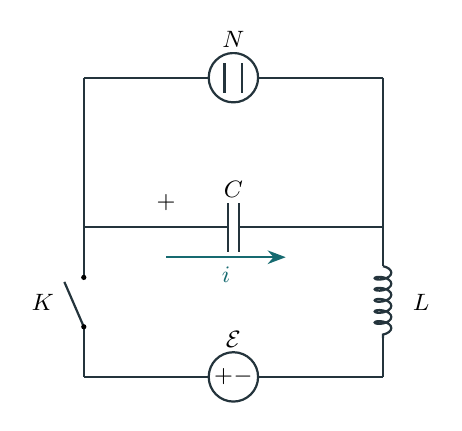
\begin{tikzpicture}[scale=.95,transform shape]
\begin{scope}[shift={(2.0,2.0)},rotate=0.0]\draw[object] (-2.0,0)--(-0.22,0) (0.22,0)--(2.0,0);\draw[object] (-.07,-.33)--(-.07,.33) (.07,-.33)--(.07,.33) (-.22,0)--(-.07,0) (.07,0)--(.22,0);\end{scope}\node[anchor=south,fill=white,inner sep=1.5pt] at (2.0000,2.3400) {$C$};
\begin{scope}[shift={(4.0,1.0)},rotate=-90.0]\draw[object] (-1.0,0)--(-0.48,0) (0.48,0)--(1.0,0);\draw[object,decorate,decoration={coil,aspect=.45,segment length=4pt,amplitude=3pt}] (-.48,0)--(.48,0);\end{scope}\node[anchor=west,fill=white,inner sep=1.5pt] at (4.3400,1.0000) {$L$};
\begin{scope}[shift={(2.0,0.0)},rotate=0.0]\draw[object] (-2.0,0)--(-0.33,0) (0.33,0)--(2.0,0);\draw[object,fill=white] (0,0) circle (.33);\node[rotate=-0.0] at (-.13,0) {$+$};\node[rotate=-0.0] at (.13,0) {$-$};\end{scope}\node[anchor=south,fill=white,inner sep=1.5pt] at (2.0000,0.3400) {$\mathcal E$};
\begin{scope}[shift={(0.0,1.0)},rotate=90.0]\draw[object] (-1.0,0)--(-0.33,0) (0.33,0)--(1.0,0);\draw[object] (-.33,0)--(.27,.26);\fill (-.33,0) circle (.035) (.33,0) circle (.035);\end{scope}\node[anchor=east,fill=white,inner sep=1.5pt] at (-0.3400,1.0000) {$K$};
\draw[object] (0,2)--(0,4);
\begin{scope}[shift={(2.0,4.0)},rotate=0.0]\draw[object] (-2.0,0)--(-0.33,0) (0.33,0)--(2.0,0);\draw[object,fill=white] (0,0) circle (.33);\draw[object] (-.12,-.2)--(-.12,.2) (.12,-.2)--(.12,.2);\end{scope}\node[anchor=south,fill=white,inner sep=1.5pt] at (2.0000,4.3400) {$N$};
\draw[object] (4,4)--(4,2);\node[above] at (1.1,2.1){$+$};\draw[motion] (1.1,1.6)--(2.7,1.6) node[midway,below]{$i$};
\end{tikzpicture}
\figcaption{图电5.3\quad 电源、无损电感与并联氖灯}
\end{minipage}\end{center}

\Needspace{6\baselineskip}\subsection*{解答}


取图电5.3中$u_C$为左极板对右极板的电压，电流$i$流入电容正极板。灯绝缘时，
\[
 L\dot i+u_C=\mathcal E,\quad i=C\dot u_C,\quad
 \ddot u_C+\omega_0^2(u_C-\mathcal E)=0,\quad\omega_0=\frac1{\sqrt{LC}}.
\]
这个方程可从电量逐步得到：令$q=Cu_C$、$i=\dot q$，回路给$\mathcal E=L\ddot q+q/C$。引入$q^*=q-C\mathcal E$，便将常量电源项移入平衡位置：
\[
\ddot q^*+\omega_0^2q^*=0,\qquad
q^*=A\cos(\omega_0t+\varphi),\qquad
i=-\omega_0A\sin(\omega_0t+\varphi).
\]
初态$q=0,i=0$要求$A\cos\varphi=-C\mathcal E$、$A\sin\varphi=0$；取正振幅得到$A=C\mathcal E,\varphi=\pi$，再还原q和uC，得到下面的第一段解。恒定电源把振动的平衡位置移到电压 $\mathcal E$。

平衡电压是$\mathcal E$。初始$u_C(0)=0,\ i(0)=0$给出
\[
 u_C=\mathcal E(1-\cos\omega_0t),\qquad
 i=C\mathcal E\omega_0\sin\omega_0t.
\]
若不点灯，第一峰达到$2\mathcal E=68\,{\rm V}>U_z$，所以灯必亮一次。

\begin{center}\begin{minipage}{.97\linewidth}\centering
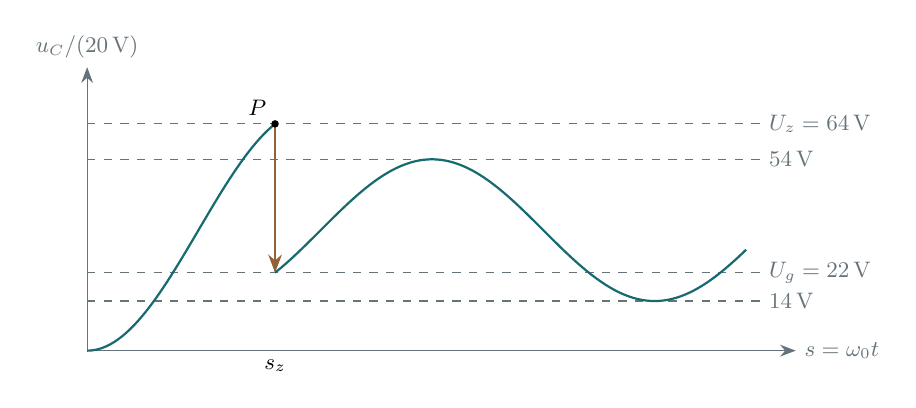
\begin{tikzpicture}[scale=.9,transform shape]
\draw[axis](0,0)--(10,0)node[right]{$s=\omega_0t$};\draw[axis](0,0)--(0,4)node[above]{$u_C/(20\,\mathrm V)$};
\draw[guide](0,3.2)--(9.5,3.2)node[right]{$U_z=64\,\mathrm V$};\draw[guide](0,2.7)--(9.5,2.7)node[right]{$54\,\mathrm V$};
\draw[guide](0,1.1)--(9.5,1.1)node[right]{$U_g=22\,\mathrm V$};\draw[guide](0,.7)--(9.5,.7)node[right]{$14\,\mathrm V$};
\draw[traj,domain=0:2.651635327336,samples=90]plot(\x,{1.7*(1-cos(deg(\x)))});
\draw[force](2.651635327336,3.2)--(2.651635327336,1.1);
\draw[traj,domain=2.651635327336:9.3,samples=170]plot(\x,{1.7-.6*cos(deg(\x-2.651635327336))+.8*sin(deg(\x-2.651635327336))});
\fill(2.651635327336,3.2)circle(1.5pt);\node[above left]at(2.651635327336,3.2){$P$};\node[below]at(2.651635327336,0){$s_z$};
\end{tikzpicture}
\figcaption{解图电5.3A　首次达到燃点P后快速降压，后续振荡始终在14至54伏之间；$s_z=\arccos(-15/17)$。}
\end{minipage}\end{center}


解图电5.3A的首次交点$P$处，$\theta_z=\omega_0t_z\in(0,\pi)$，有
\[
 \cos\theta_z=1-\frac{64}{34}=-\frac{15}{17},\qquad
 \sin\theta_z=\frac8{17},\qquad i_z=16C\omega_0 .
\]
放电使$u_C$从$64$降至$22\,{\rm V}$，却不改变$i_z$。以熄灭时为$t'=0$，新的初始条件是
$u_C(0)=22\,{\rm V},\ \dot u_C(0)=(16\,{\rm V})\omega_0$。因此
\[
 u_C(t')=34-12\cos\omega_0t'+16\sin\omega_0t'\quad({\rm V}).
\]
若按电量的通解重新求常数，可写
\[
q'=C\mathcal E+A'\cos(\omega_0t'+\varphi'),\qquad
i'=-\omega_0A'\sin(\omega_0t'+\varphi').
\]
放电后初值必须同时保留电压和电流，故
\[
\frac{A'}C\cos\varphi'=U_g-\mathcal E=-12\,\mathrm V,\qquad
\frac{A'}C\sin\varphi'=-\frac{i_z}{C\omega_0}=-16\,\mathrm V.
\]
两式平方相加给$A'/C=20\,\mathrm V$，并有$\cos\varphi'=-3/5,\sin\varphi'=-4/5$。可选$\varphi'=-\arccos(-3/5)$，展开余弦恰恢复上面的$-12\cos\omega_0t'+16\sin\omega_0t'$；正弦项来自熄灭时仍存在线圈电流 $i_z=(16\,\mathrm V)C\omega_0$，它给出初始升压斜率 $(16\,\mathrm V)\omega_0$。

相对中心$34\,{\rm V}$的振幅为$\sqrt{12^2+16^2}=20\,{\rm V}$，所以
\[
 \boxed{14\,{\rm V}\le u_C(t')\le54\,{\rm V}<64\,{\rm V}.}
\]
后续任意时刻够不到燃点，灯不再点亮。

\begin{center}\begin{minipage}{.97\linewidth}\centering
\begin{tikzpicture}[scale=.95,transform shape,font=\small]
\draw[axis](-2.3,0)--(2.5,0);\draw[axis](0,-2.05)--(0,2.35)node[above]{$y=i/(20C\omega_0\,\mathrm V)$};
\node[below]at(.3,-2.2){$x=(u_C-\mathcal E)/(20\,\mathrm V)$};
\draw[object](0,0)circle(1.7);\draw[traj](0,0)circle(1);
\draw[guide](1.5,-1.9)--(1.5,2.05);\node[above right]at(1.5,2.05){$u_C=U_z$};
\fill(-1.7,0)circle(1.6pt) (1.5,.8)circle(1.6pt) (-.6,.8)circle(1.6pt);
\node[below left]at(-1.7,0){$S$};\node[above right]at(1.5,.8){$P$};\node[above left]at(-.6,.8){$Q$};
\draw[force](1.5,.8)--(-.6,.8);\node at(.45,1.3){放电};
\draw[motion](130:1.7)arc(130:110:1.7);\draw[motion](-60:1)arc(-60:-85:1);
\node[align=left,anchor=west]at(3.1,.7){$S=(-17/10,0)$\\$P=(3/2,4/5)$\\$Q=(-3/5,4/5)$\\外圆半径$17/10$\\内圆半径$1$\\横向跳跃，纵坐标不变};
\end{tikzpicture}
\figcaption{解图电5.3B　两个状态分量均按20伏归一化。大圆到P后保持电流跳到Q，小圆沿顺时针运动，始终达不到燃点线。}
\end{minipage}\end{center}


解图电5.3B将电压变量$(u_C-\mathcal E,\ i/(C\omega_0))$各除以$20\,\mathrm V$绘图。若以伏写未归一化的对应值，先沿半径$34\,{\rm V}$的圆到$P=(30,16)$；放电只改变横坐标，跳到$Q=(-12,16)$；此后沿半径$20\,{\rm V}$的圆运动，达不到燃点线$u_C-\mathcal E=30\,{\rm V}$。

在小圆上，熄灭后$\tfrac12C(u_C-\mathcal E)^2+\tfrac12Li^2$守恒。它是平移后的振动能；实际电容能$\tfrac12Cu_C^2$与磁能之和还要计入电源功。

\begin{center}\begin{minipage}{.97\linewidth}\centering
\begin{tikzpicture}[scale=.9,transform shape,font=\small]
\draw[axis](0,0)--(6,0);\draw[axis](0,0)--(0,4.9)node[above]{$W/(C\,\mathrm V^2)$};
\foreach \val in {1000,2000}{\draw(-.07,{\val/512})--(.07,{\val/512});\node[left]at(0,{\val/512}){$\val$};}
\fill[accent!25](.7,0)rectangle(1.8,4);\fill[warm!50](.7,4)rectangle(1.8,4.25);
\fill[accent!25](3.8,0)rectangle(4.9,{242/512});\fill[warm!50](3.8,{242/512})rectangle(4.9,{370/512});
\node[above]at(1.25,4.3){$2176$};\node[above]at(4.35,{370/512+.1}){$370$};
\node[below,align=center]at(1.25,0){放电前P\\$W_C=2048C\,\mathrm V^2$\\$W_L=128C\,\mathrm V^2$};
\node[below,align=center]at(4.35,0){放电后Q\\$W_C=242C\,\mathrm V^2$\\$W_L=128C\,\mathrm V^2$};
\node[align=left,anchor=west]at(6.2,2.7){蓝色：真实电场能\\橙色：磁场能\\短暂放电中磁能不变\\电源功趋于零\\灯中释放$1806C\,\mathrm V^2$};
\end{tikzpicture}
\figcaption{解图电5.3C　P到Q的储能变化。电容场能减少，线圈电流保持，因此磁能保持。}
\end{minipage}\end{center}

解图电5.3C逐项使用真实储能：P处电容能$C(64\,\mathrm V)^2/2=2048C\,\mathrm V^2$，磁能为$Li_z^2/2=128C\,\mathrm V^2$；Q处电容能降为$C(22\,\mathrm V)^2/2=242C\,\mathrm V^2$，磁能不变。放电用时趋于零而串联电流有限，电源在该短时段的功趋于零，故灯中释放$1806C\,\mathrm V^2$。

图B对应的平移振动能是
\[
\mathcal H_{\rm osc}=\frac12C(u_C-\mathcal E)^2+\frac12Li^2
=\left(\frac12Cu_C^2+\frac12Li^2\right)-C\mathcal E u_C+\frac12C\mathcal E^2.
\]
灯灭的每段都满足其导数为零，因电源做功项已被移入平衡点。P到Q时它只减少$(34^2-20^2)C\,\mathrm V^2/2=378C\,\mathrm V^2$，与真实耗散相差$C\mathcal E(U_z-U_g)=1428C\,\mathrm V^2$；前者描述图B圆半径的改变，灯的热量由图C所示的实际电容能差给出。灯灭时，实际储能随电源功变化，平移后的振动能守恒。


\Needspace{13\baselineskip}

\pdfbookmark[2]{第 4 题 任意波形下保持平衡的电感电桥}{q4}

\section*{第 4 题\quad 任意波形下保持平衡的电感电桥}\label{q:4}


电桥由两条串联支路并联于电源两端。上支路依次为$(L_1,R_1)$和$R_3$，下支路依次为$(L_2,R_2)$和$R_4$；两个中点之间接电流计$M$。选择元件，使任意电动势$\mathcal E(t)$下电流计均无电流（从相容初态出发，电感互感忽略）。已知$R_2=90\,\Omega$，$R_3=300\,\Omega$，$R_4=60\,\Omega$，$L_2=900\,{\rm mH}$，求$R_1,L_1$。

\begin{center}\begin{minipage}{.98\linewidth}\centering
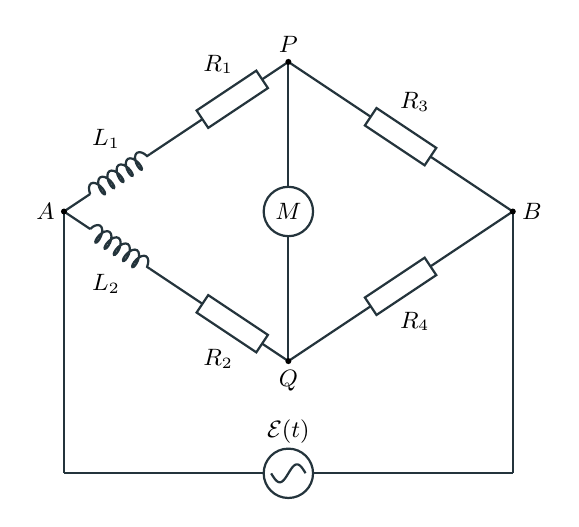
\begin{tikzpicture}[scale=.95,transform shape]
\begin{scope}[shift={(0.75,0.5)},rotate=33.690067525979785]\draw[object] (-0.9013878188659973,0)--(-0.48,0) (0.48,0)--(0.9013878188659973,0);\draw[object,decorate,decoration={coil,aspect=.45,segment length=4pt,amplitude=3pt}] (-.48,0)--(.48,0);\end{scope}\node[anchor=south,fill=white,inner sep=1.5pt] at (0.5614,0.7829) {$L_1$};
\begin{scope}[shift={(2.25,1.5)},rotate=33.690067525979785]\draw[object] (-0.9013878188659973,0)--(-0.48,0) (0.48,0)--(0.9013878188659973,0);\draw[object,fill=white] (-.48,-.14) rectangle (.48,.14);\end{scope}\node[anchor=south,fill=white,inner sep=1.5pt] at (2.0614,1.7829) {$R_1$};
\begin{scope}[shift={(4.5,1.0)},rotate=-33.690067525979785]\draw[object] (-1.8027756377319946,0)--(-0.48,0) (0.48,0)--(1.8027756377319946,0);\draw[object,fill=white] (-.48,-.14) rectangle (.48,.14);\end{scope}\node[anchor=south,fill=white,inner sep=1.5pt] at (4.6886,1.2829) {$R_3$};
\begin{scope}[shift={(0.75,-0.5)},rotate=-33.690067525979785]\draw[object] (-0.9013878188659973,0)--(-0.48,0) (0.48,0)--(0.9013878188659973,0);\draw[object,decorate,decoration={coil,aspect=.45,segment length=4pt,amplitude=3pt}] (-.48,0)--(.48,0);\end{scope}\node[anchor=north,fill=white,inner sep=1.5pt] at (0.5614,-0.7829) {$L_2$};
\begin{scope}[shift={(2.25,-1.5)},rotate=-33.690067525979785]\draw[object] (-0.9013878188659973,0)--(-0.48,0) (0.48,0)--(0.9013878188659973,0);\draw[object,fill=white] (-.48,-.14) rectangle (.48,.14);\end{scope}\node[anchor=north,fill=white,inner sep=1.5pt] at (2.0614,-1.7829) {$R_2$};
\begin{scope}[shift={(4.5,-1.0)},rotate=33.690067525979785]\draw[object] (-1.8027756377319946,0)--(-0.48,0) (0.48,0)--(1.8027756377319946,0);\draw[object,fill=white] (-.48,-.14) rectangle (.48,.14);\end{scope}\node[anchor=north,fill=white,inner sep=1.5pt] at (4.6886,-1.2829) {$R_4$};
\begin{scope}[shift={(3.0,0.0)},rotate=-90.0]\draw[object] (-2.0,0)--(-0.33,0) (0.33,0)--(2.0,0);\draw[object,fill=white] (0,0) circle (.33);\node[rotate=90.0] at (0,0) {$M$};\end{scope}
\draw[object] (0,0)--(0,-3.5);
\draw[object] (6,0)--(6,-3.5);
\begin{scope}[shift={(3.0,-3.5)},rotate=0.0]\draw[object] (-3.0,0)--(-0.33,0) (0.33,0)--(3.0,0);\draw[object,fill=white] (0,0) circle (.33);\draw[object] plot[domain=-.23:.23,samples=35] (\x,{.12*sin(780*\x)});\end{scope}\node[anchor=south,fill=white,inner sep=1.5pt] at (3.0000,-3.1600) {$\mathcal E(t)$};\fill (0,0) circle(.04);\node[left] at (0,0) {$A$};\fill (3,2) circle(.04);\node[above] at (3,2) {$P$};\fill (3,-2) circle(.04);\node[below] at (3,-2) {$Q$};\fill (6,0) circle(.04);\node[right] at (6,0) {$B$};
\end{tikzpicture}
\figcaption{图电5.4\quad 两组$RL$臂与纯电阻臂构成电桥}
\end{minipage}\end{center}

\Needspace{6\baselineskip}\subsection*{解答}


先看电动势已经不随时间变化的直流稳态，电感压降为零。桥中无电流时，右侧$R_3i_1=R_4i_2$，左侧$R_1i_1=R_2i_2$，故
\[
R_1R_4=R_2R_3,\qquad R_1=\frac{R_2R_3}{R_4}=450\,\Omega.
\]
电阻由直流稳态给定。接下来保留电感的导数项，求随时间变化的电源下的平衡条件。

图电5.4的中点为$P,Q$。若电流计无电流，两支路电流为$i_1,i_2$，且$V_P=V_Q$。比较右侧电阻和左侧$RL$电压，得
\[
 R_3i_1=R_4i_2,\qquad
 L_1\dot i_1+R_1i_1=L_2\dot i_2+R_2i_2 .
\]
由$i_2=(R_3/R_4)i_1$代入，
\[
 \left(L_1-\frac{R_3}{R_4}L_2\right)\dot i_1+
 \left(R_1-\frac{R_3}{R_4}R_2\right)i_1=0 .
\]
直流稳态使 $\dot i_1=0$，非零电流给电阻系数为零；接入阶跃后 $\dot i_1$ 非零，故导数系数也为零：
\[
 \boxed{\frac{R_1}{R_2}=\frac{L_1}{L_2}=\frac{R_3}{R_4}=5.}
\]
所以
\[
 \boxed{R_1=450\,\Omega,\qquad L_1=4500\,{\rm mH}=4.50\,{\rm H}.}
\]

\begin{center}\begin{minipage}{.98\linewidth}\centering
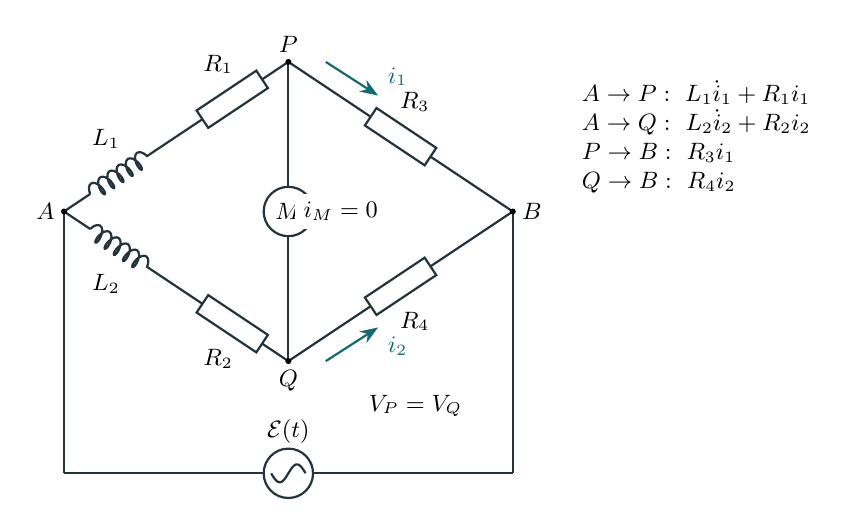
\begin{tikzpicture}[scale=.95,transform shape]
\begin{scope}[shift={(0.75,0.5)},rotate=33.690067525979785]\draw[object] (-0.9013878188659973,0)--(-0.48,0) (0.48,0)--(0.9013878188659973,0);\draw[object,decorate,decoration={coil,aspect=.45,segment length=4pt,amplitude=3pt}] (-.48,0)--(.48,0);\end{scope}\node[anchor=south,fill=white,inner sep=1.5pt] at (0.5614,0.7829) {$L_1$};
\begin{scope}[shift={(2.25,1.5)},rotate=33.690067525979785]\draw[object] (-0.9013878188659973,0)--(-0.48,0) (0.48,0)--(0.9013878188659973,0);\draw[object,fill=white] (-.48,-.14) rectangle (.48,.14);\end{scope}\node[anchor=south,fill=white,inner sep=1.5pt] at (2.0614,1.7829) {$R_1$};
\begin{scope}[shift={(4.5,1.0)},rotate=-33.690067525979785]\draw[object] (-1.8027756377319946,0)--(-0.48,0) (0.48,0)--(1.8027756377319946,0);\draw[object,fill=white] (-.48,-.14) rectangle (.48,.14);\end{scope}\node[anchor=south,fill=white,inner sep=1.5pt] at (4.6886,1.2829) {$R_3$};
\begin{scope}[shift={(0.75,-0.5)},rotate=-33.690067525979785]\draw[object] (-0.9013878188659973,0)--(-0.48,0) (0.48,0)--(0.9013878188659973,0);\draw[object,decorate,decoration={coil,aspect=.45,segment length=4pt,amplitude=3pt}] (-.48,0)--(.48,0);\end{scope}\node[anchor=north,fill=white,inner sep=1.5pt] at (0.5614,-0.7829) {$L_2$};
\begin{scope}[shift={(2.25,-1.5)},rotate=-33.690067525979785]\draw[object] (-0.9013878188659973,0)--(-0.48,0) (0.48,0)--(0.9013878188659973,0);\draw[object,fill=white] (-.48,-.14) rectangle (.48,.14);\end{scope}\node[anchor=north,fill=white,inner sep=1.5pt] at (2.0614,-1.7829) {$R_2$};
\begin{scope}[shift={(4.5,-1.0)},rotate=33.690067525979785]\draw[object] (-1.8027756377319946,0)--(-0.48,0) (0.48,0)--(1.8027756377319946,0);\draw[object,fill=white] (-.48,-.14) rectangle (.48,.14);\end{scope}\node[anchor=north,fill=white,inner sep=1.5pt] at (4.6886,-1.2829) {$R_4$};
\begin{scope}[shift={(3.0,0.0)},rotate=-90.0]\draw[object] (-2.0,0)--(-0.33,0) (0.33,0)--(2.0,0);\draw[object,fill=white] (0,0) circle (.33);\node[rotate=90.0] at (0,0) {$M$};\end{scope}
\draw[object] (0,0)--(0,-3.5);
\draw[object] (6,0)--(6,-3.5);
\begin{scope}[shift={(3.0,-3.5)},rotate=0.0]\draw[object] (-3.0,0)--(-0.33,0) (0.33,0)--(3.0,0);\draw[object,fill=white] (0,0) circle (.33);\draw[object] plot[domain=-.23:.23,samples=35] (\x,{.12*sin(780*\x)});\end{scope}\node[anchor=south,fill=white,inner sep=1.5pt] at (3.0000,-3.1600) {$\mathcal E(t)$};\fill (0,0) circle(.04);\node[left] at (0,0) {$A$};\fill (3,2) circle(.04);\node[above] at (3,2) {$P$};\fill (3,-2) circle(.04);\node[below] at (3,-2) {$Q$};\fill (6,0) circle(.04);\node[right] at (6,0) {$B$};
\draw[motion] (3.5,2)--(4.2,1.55) node[above right]{$i_1$};
\draw[motion] (3.5,-2)--(4.2,-1.55) node[below right]{$i_2$};
\node[fill=white] at (4.7,-2.6){$V_P=V_Q$};
\node[align=left,anchor=west]at(6.8,1){$A\to P:\ L_1\dot i_1+R_1i_1$\\$A\to Q:\ L_2\dot i_2+R_2i_2$\\$P\to B:\ R_3i_1$\\$Q\to B:\ R_4i_2$};
\node[fill=white]at(3.7,0){$i_M=0$};

\end{tikzpicture}
\figcaption{解图电5.4A\quad 桥平衡要求右侧压降及左侧$RL$压降分别相同}
\end{minipage}\end{center}

解图电5.4A在实际支路旁列出两侧压降，以$V_P=V_Q$分别比较；等势是电流计无流时的结果。对任意频率$\Omega$，也可写
\[
 \frac{R_1+j\Omega L_1}{R_2+j\Omega L_2}=\frac{R_3}{R_4}.
\]
实部给电阻比例，虚部给电感比例，两者同时成立时各频率均平衡，零频直流也包括在内。

接着比较两支路的初始电流。令$k=R_3/R_4$，平衡轨道要求$i_2(0)=k i_1(0)$。从全无电流时接入任意驱动满足该条件；若人为预存不同比例的电感电流，它们的自由响应就在电流计中产生一段衰减电流。


零初态接通阶跃时，两支路以同一时间常数建立电流。给电源一个幅值$E_s>0$的阶跃，两条主支路在平衡轨道上分别满足
\[
L_1\dot i_1+(R_1+R_3)i_1=E_s,\qquad
L_2\dot i_2+(R_2+R_4)i_2=E_s.
\]
匹配数值给$R_1+R_3=750\,\Omega$、$R_2+R_4=150\,\Omega$，所以
\[
\tau=\frac{4.5\,\mathrm H}{750\,\Omega}=\frac{0.9\,\mathrm H}{150\,\Omega}
=0.006\,\mathrm s,\quad
i_1=\frac{E_s}{750\,\Omega}(1-e^{-t/\tau}),\quad i_2=5i_1.
\]
\begin{center}\begin{minipage}{.97\linewidth}\centering
\begin{tikzpicture}[scale=.85,transform shape,font=\small]
\draw[axis](0,0)--(5.3,0)node[right]{$t/\tau$};\draw[axis](0,0)--(0,5.8)node[above]{$i/[E_s/(750\,\Omega)]$};
\draw[guide](0,1)--(4.7,1);\draw[guide](0,5)--(4.7,5);
\node[left]at(0,1){$1$};\node[left]at(0,5){$5$};
\draw[blue,thick,domain=0:4.6,samples=85]plot(\x,{1-exp(-\x)});
\draw[orange!80!black,thick,domain=0:4.6,samples=85]plot(\x,{5*(1-exp(-\x))});
\node[right]at(4.7,.98){$i_1$};\node[right]at(4.7,4.95){$i_2$};
\node[align=left,anchor=west]at(6.2,3){输入$E_s$阶跃，初始电流零\\两支路均以$\tau=6\,\mathrm{ms}$趋稳\\任意时刻$i_2=5i_1$\\$V_P=V_Q=\frac25E_s(1-e^{-t/\tau})$};
\end{tikzpicture}
\figcaption{解图电5.4B　零初态阶跃的两支路实际电流。它们幅值不同而时间尺度相同，因此从启动瞬间到稳态都保持平衡。}
\end{minipage}\end{center}

解图电5.4B中的较高曲线是下支路的 $i_2$，其值始终为上支路电流 $i_1$ 的5倍。右侧压降分别为$300i_1$与$60i_2$，代入全程相等；左侧压降也随同比例算子相等。同一阻抗比例给出正弦稳态平衡，也使图B的阶跃过程全程平衡。任意输入可以由线性响应叠加，而时域的算子证明已直接给出所有波形的共同条件。

下面保留电流计支路，计算初始电流失配后的表流。设其内阻$R_g>0$、表流$i_M$取P到Q；仍把$i_1,i_2$定义为左侧两条RL臂中的电流。表流不为零时，右侧电阻电流分别是$i_1-i_M$和$i_2+i_M$，节点守恒给
\[
i_M=\frac{R_3i_1-R_4i_2}{D_g},\quad D_g=R_g+R_3+R_4,
\quad\delta=i_2-ki_1,\quad i_M=-\frac{R_4}{D_g}\delta.
\]
两条含电感的实际回路式相减，并用$L_1=kL_2,R_1=kR_2$，得到
\[
L_2\dot\delta+R_2\delta+V_Q-V_P=0,\qquad
V_Q-V_P=-R_gi_M=\frac{R_gR_4}{D_g}\delta.
\]
因此
\[
\dot\delta=-\frac{R_2+R_gR_4/D_g}{L_2}\delta,\qquad
i_M(t)=-\frac{R_4\delta(0)}{D_g}e^{-t/\tau_\delta},\quad
\tau_\delta=\frac{L_2}{R_2+R_gR_4/D_g}.
\]
输入电动势在差式中消去。若初始失配为零，表流就对任意驱动恒为零；若初始失配不为零，即使元件比例已经正确，仍会有一段由预存电流产生的表流。失配方程给出了这两种初态各自的明确判据。
\begin{center}\begin{minipage}{.97\linewidth}\centering
\begin{tikzpicture}[x=.12cm,y=4cm,font=\small]
\draw[axis](0,0)--(45,0)node[right]{$t/\mathrm{ms}$};\draw[axis](0,0)--(0,.8)node[above]{$i_M/\mathrm A$};
\foreach \x in {10,20,30,40}{\draw(\x,0)--(\x,-.015);\node[below]at(\x,-.02){$\x$};}
\foreach \y in {.2,.4,.6}{\draw(0,\y)--(-.7,\y);\node[left]at(-.7,\y){$\y$};}
\draw[traj,domain=0:40,samples=100]plot(\x,{(15/23)*exp(-(79/690)*\x)});
\node[align=left,anchor=west]at(49,.43){$R_g=100\,\Omega$\\$i_1(0)=1\,\mathrm A,\ i_2(0)=0$\\$i_M(0)=15/23\,\mathrm A$\\$\tau_\delta=69/7900\,\mathrm s$\\相容初态的表流始终为零\\图中是初始失配的自由响应};
\end{tikzpicture}
\figcaption{解图电5.4C　元件匹配而初始电流不匹配时的实际表流。曲线取正方向P到Q；它由自由响应决定，与共同施加的电动势波形无关。}
\end{minipage}\end{center}

解图电5.4C采用$R_g=100\,\Omega,i_1(0)=1\,\mathrm A,i_2(0)=0$，故$\delta(0)=-5\,\mathrm A$，$i_M(0)=15/23\,\mathrm A$，随后按时间常数$69/7900\,\mathrm s$衰减。图B从全无电流的相容初态出发，图C从预存电流的失配初态出发。


\Needspace{13\baselineskip}

\pdfbookmark[2]{第 5 题 三元件黑盒的连接与参数识别}{q5}

\section*{第 5 题\quad 三元件黑盒的连接与参数识别}\label{q:5}


一个两端黑盒内只有电阻$R$、理想电感$L$和理想电容$C$各一只。接$100\,{\rm V}$直流电压时电流为$0.1\,{\rm A}$；接频率$60\,{\rm Hz}$、有效值$100\,{\rm V}$的交流电压时电流有效值为$1\,{\rm A}$。频率增至$1000\,{\rm Hz}$时，电流达到很大的极大值。判断连接方式，并求元件数值；讨论这些测量是否足以唯一确定网络。

\begin{center}\begin{minipage}{.98\linewidth}\centering
\begin{tikzpicture}[scale=.95,transform shape]

\draw[object] (0,0) rectangle (4,2);\draw[object] (-1,1)--(0,1) (4,1)--(5,1);
\fill (-1,1) circle(.04) (5,1) circle(.04);
\node at (2,1.35){$R,L,C$各一只};\node at (2,.65){内部连接待定};
\node[left] at (-1,1){$A$};\node[right] at (5,1){$B$};

\end{tikzpicture}
\figcaption{图电5.5\quad 根据端口的直流、交流和峰频测量反推网络}
\end{minipage}\end{center}

\Needspace{6\baselineskip}\subsection*{解答}


先约定三个元件均实际接入端口A、B之间，且不计无作用的悬空支路、导线短接或隐藏的第四个元件。三元件两端网络的不同串并联结构可列为：全部串联、全部并联，以及“一个元件与另两个串联支路并联”和“一个元件与另两个并联部分串联”各三种，共八类。将三只元件画成三角形、再只从两个顶点接出端口，第三顶点是内部节点，仍归入其中的一个元件并联另两元件串联。

直流稳态中，电容开路、电感短路。全部串联和$C+(R\parallel L)$均被电容截断，端口电流应为零；全部并联和$L\parallel(R+C)$均被电感直接短接，不能得到给定的有限电流。$R+(L\parallel C)$ 的串联电抗是 $X_p=\Omega L/(1-\Omega^2LC)$。谐振下方 $X_p$ 从0增至正无穷；谐振上方从负无穷增至0。因此 $U/\sqrt{R^2+X_p^2}$ 先降后升，谐振点是电流谷，两个区间都没有电流峰。这五类分别由实际路径排除，接下来对其余三类逐一算频率响应。

三个元件都参与两端网络，非零且有限的直流电流意味着：电容不能阻断全部直流路径，电感不能单独跨接端口。图电5.5先保留未知结构，直流筛选后只剩三类：
\[
 C\parallel(R+L),\qquad L+(R\parallel C),\qquad R\parallel(L+C).
\]
第一类$Y=1/(R+j\Omega L)+j\Omega C$。令$x=\Omega^2$，则
\[
 |Y|^2=C^2x+\frac{1-2LCx}{R^2+L^2x},\quad
 \frac{\dd|Y|^2}{\dd x}
 =C^2-\frac{2LCR^2+L^2}{(R^2+L^2x)^2}.
\]
导数随$x$单调增加，可能有电流谷值，没有有限频率的内部极大，可排除。其余两类需要定量检查。这里还可直接求二阶导数：$\dd^2|Y|^2/\dd x^2=2L^2(2LCR^2+L^2)/(R^2+L^2x)^3>0$。端口电压有效值固定，$I^2=U^2|Y|^2$，因此导纳模平方的凸性确实排除了内部电流峰，导数变号时只会从负变正，对应的是电流谷。

\begin{center}\begin{minipage}{.98\linewidth}\centering
\begin{tikzpicture}[scale=.95,transform shape]
\draw[object] (0,1)--(0,3);
\begin{scope}[shift={(3.0,3.0)},rotate=0.0]\draw[object] (-3.0,0)--(-0.48,0) (0.48,0)--(3.0,0);\draw[object,fill=white] (-.48,-.14) rectangle (.48,.14);\end{scope}\node[anchor=south,fill=white,inner sep=1.5pt] at (3.0000,3.3400) {$R$};
\draw[object] (6,3)--(6,1);
\draw[object] (0,1)--(0,0);
\begin{scope}[shift={(1.5,0.0)},rotate=0.0]\draw[object] (-1.5,0)--(-0.48,0) (0.48,0)--(1.5,0);\draw[object,decorate,decoration={coil,aspect=.45,segment length=4pt,amplitude=3pt}] (-.48,0)--(.48,0);\end{scope}\node[anchor=south,fill=white,inner sep=1.5pt] at (1.5000,0.3400) {$L$};
\begin{scope}[shift={(4.5,0.0)},rotate=0.0]\draw[object] (-1.5,0)--(-0.22,0) (0.22,0)--(1.5,0);\draw[object] (-.07,-.33)--(-.07,.33) (.07,-.33)--(.07,.33) (-.22,0)--(-.07,0) (.07,0)--(.22,0);\end{scope}\node[anchor=south,fill=white,inner sep=1.5pt] at (4.5000,0.3400) {$C$};
\draw[object] (6,0)--(6,1);\fill (0,1) circle(.04);\node[left] at (0,1) {$A$};\fill (6,1) circle(.04);\node[right] at (6,1) {$B$};\begin{scope}[shift={(8.0,.1)}]
\draw[axis](-.2,0)--(2.3,0)node[right]{$\Re$};\draw[axis](0,-.15)--(0,3.2)node[above]{$\Im$};
\draw[motion](0,0)--(.28,0);\draw[force](0,0)--(0,2.78596);
\draw[traj,-{Stealth}](0,0)--(.28,2.78596);
\draw[guide](.28,0)--(.28,2.78596)--(0,2.78596);
\node[align=left,anchor=west]at(.75,1.6){以端口电压为实轴\\$I_R=0.100\,\mathrm A$\\$I_{LC}=\sqrt{.99}\,\mathrm A$\\$I=1.000\,\mathrm A$};
\node[below]at(.3,-.2){横、纵方向采用相同标度};
\node[above]at(1,3.5){$60\,\mathrm{Hz}:\ X<0$};
\end{scope}
\end{tikzpicture}
\figcaption{解图电5.5A\quad 第一组可行连接及正交电流}
\end{minipage}\end{center}

先取解图电5.5A的$R\parallel(L+C)$。直流只经电阻，
\[
 R=\frac{100}{0.1}=1000\,\Omega.
\]
记$X=\Omega L-1/(\Omega C)$。并联电阻电流与$LC$电流正交，故
\[
 I^2=(U/R)^2+(U/X)^2.
\]
在$60\,{\rm Hz}$，$|X|=100/\sqrt{1-0.1^2}=100.5038\,\Omega$。在$1000\,{\rm Hz}$串联谐振，$LC=\Omega_r^{-2}$。由于$60<1000$，$X<0$，于是
\[
 \frac{1-(60/1000)^2}{\Omega_{60}C}=100.5038\,\Omega.
\]
解得
\[
 \boxed{R=1000\,\Omega,\quad C=26.2978\,\mu{\rm F},\quad
 L=0.963208\,{\rm mH}.}
\]
理想模型谐振处阻抗为零；实际小损耗会把无界电流限制为很大的有限峰值。

解图电5.5A右侧相量图以端口电压为实轴，箭头长度按电流有效值画出。$60\,\mathrm{Hz}$时$LC$支路呈容性，故支流超前电压$90^\circ$，总相量为$\underline I=(0.1+\mathrm j\sqrt{.99})\,\mathrm A$，其模为1安。电阻电流只有总电流的十分之一，所以图中的竖向投影远大于横向投影。若取端口电压为$\underline U=100\,\mathrm V$，则$\underline Z=\underline U/\underline I=(10-\mathrm j\,99.4987)\,\Omega$。

复阻抗法还应把从测量到参数的代数写出。设$Z_0=100\,\Omega$、$\Omega_0=2\pi(60\,\mathrm{Hz})$，由两条并联支路
\[
\frac1{\underline Z}=\frac1R+\frac1{\mathrm jX},\qquad
|\underline Z|=\frac{R|X|}{\sqrt{R^2+X^2}},\qquad
|X_0|=\frac{Z_0R}{\sqrt{R^2-Z_0^2}}.
\]
串联谐振给$LC=1/\Omega_r^2$，而$\Omega_0<\Omega_r$使$X_0=(\Omega_0^2LC-1)/(\Omega_0C)<0$，从而
\[
C=\frac{(1-\Omega_0^2LC)\sqrt{R^2-Z_0^2}}{\Omega_0 Z_0R}
=\frac{[1-(60/1000)^2]\sqrt{.99}}{100\,\Omega\cdot\Omega_0},
\qquad L=\frac1{\Omega_r^2C}.
\]
括号$1-\Omega_0^2LC$为正，电容因而为正；上述反解取低频的容性支，即 $X_0=-|X_0|$。数值保留两位有效数字即$C=2.6\times10^{-5}\,\mathrm F$、$L=0.96\times10^{-3}\,\mathrm H$，与前面的精确计算相容。


但是，“很大的极大值”若只是定性有限测量，尚不能唯一排除解图电5.5B的$L+(R\parallel C)$。对它，直流仍有$R=1000\,\Omega$，而
\[
 Z=j\Omega L+\frac R{1+j\Omega RC}.
\]
令$x=\Omega RC$、$a=L/(R^2C)>0$，得到
\[
 \frac{|Z|^2}{R^2}=a^2x^2+\frac{1-2ax^2}{1+x^2}.
\]
电流峰值的条件是模的极小，不是单独$\Im Z=0$。为求出这个极小值，令$y=x^2$、$F(y)=|Z|^2/R^2$，则
\[
F'(y)=a^2-\frac{1+2a}{(1+y)^2},\qquad
F''(y)=\frac{2(1+2a)}{(1+y)^3}>0.
\]
只要驻点$y=z>0$，它就是阻抗模平方的严格唯一极小，对应电流的严格极大；两端频率极限还会确认这一点。令$z=(\Omega_rRC)^2$，求导得
\[
 a^2=\frac{1+2a}{(1+z)^2},\qquad
 a=\frac{1+\sqrt{1+(1+z)^2}}{(1+z)^2}.
\]
再令$q=(60/1000)^2=0.0036$，$60\,{\rm Hz}$测量要求
\[
 a^2qz+\frac{1-2aqz}{1+qz}=0.01 .
\]
这组方程有正数解$z\approx27300.364,\ a\approx3.66295\times10^{-5}$，对应
\[
 C\approx26.2969\,\mu{\rm F},\qquad L\approx0.963243\,{\rm mH}.
\]
代入得到直流$0.1\,{\rm A}$、$60\,{\rm Hz}$电流$1\,{\rm A}$，在$1000\,{\rm Hz}$电流约$2730\,{\rm A}$且为极大。这个有限的巨大峰同样满足定性陈述。相应峰处$\underline Z\approx(0.0366282+\mathrm j\,0.000221678)\,\Omega$，实部、虚部均不是零。由$F''>0$和$x^2$随正频率单调增加，峰的性质已被判定；$\Omega\to0$时$Z\to R$，$\Omega\to\infty$时$|Z|\sim\Omega L$，并不另有更大的有限频率电流峰。用$\Im Z=0$算出的频率约$999.9817\,\mathrm{Hz}$，与1000赫兹的电流峰很接近却不相等。

\begin{center}\begin{minipage}{.98\linewidth}\centering
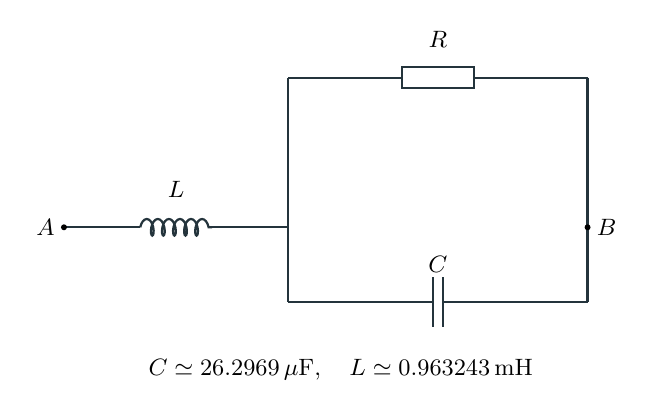
\begin{tikzpicture}[scale=.95,transform shape]
\begin{scope}[shift={(1.5,1.0)},rotate=0.0]\draw[object] (-1.5,0)--(-0.48,0) (0.48,0)--(1.5,0);\draw[object,decorate,decoration={coil,aspect=.45,segment length=4pt,amplitude=3pt}] (-.48,0)--(.48,0);\end{scope}\node[anchor=south,fill=white,inner sep=1.5pt] at (1.5000,1.3400) {$L$};
\draw[object] (3,1)--(3,3);
\begin{scope}[shift={(5.0,3.0)},rotate=0.0]\draw[object] (-2.0,0)--(-0.48,0) (0.48,0)--(2.0,0);\draw[object,fill=white] (-.48,-.14) rectangle (.48,.14);\end{scope}\node[anchor=south,fill=white,inner sep=1.5pt] at (5.0000,3.3400) {$R$};
\draw[object] (7,3)--(7,1);
\draw[object] (3,1)--(3,0);
\begin{scope}[shift={(5.0,0.0)},rotate=0.0]\draw[object] (-2.0,0)--(-0.22,0) (0.22,0)--(2.0,0);\draw[object] (-.07,-.33)--(-.07,.33) (.07,-.33)--(.07,.33) (-.22,0)--(-.07,0) (.07,0)--(.22,0);\end{scope}\node[anchor=south,fill=white,inner sep=1.5pt] at (5.0000,0.3400) {$C$};
\draw[object] (7,0)--(7,1);\fill (0,1) circle(.04);\node[left] at (0,1) {$A$};\fill (7,1) circle(.04);\node[right] at (7,1) {$B$};\node at (3.7,-.9){$C\simeq26.2969\,\mu{\rm F},\quad L\simeq0.963243\,{\rm mH}$};
\end{tikzpicture}
\figcaption{解图电5.5B\quad 同样满足有限测量的另一种连接}
\end{minipage}\end{center}

峰值的读数决定采用哪一种解释。若要求严格由题设三个理想元件产生\emph{有限}峰，只有图B给出这一类峰；图A的理想谐振为零阻抗。若“很大”只标记锐峰位置，真实峰高可由未计入的微小损耗限制，图A也是常用解释。若直接给定谐振处严格零阻抗，则图B的 $\Re Z=R/[1+(\Omega RC)^2]>0$ 将它排除。

图B的参数反解在本题数据下也只有一组。写 $t=1+z$、$w=1+qz$，因实部 $R/w$ 不超过60赫兹的阻抗模 $R/10$，可先取 $w\ge10$，即 $z\ge2500$。此区间内 $a'=-a^2t/\sqrt{1+t^2}$，所以 $|a'|<a^2$。令 $G(z)=F(qz,a(z))$，上式给 $G'=qa^2(1-t^2/w^2)+2qz(a-1/w)a'$。第二项至多为 $2qza^2/w$，而 $t^2-w^2-2zw=(1-2q-q^2)z^2-2qz>0$，故 $G'<0$。这样在含全部可行根的区间内，代入给出的正根即可确定唯一参数。


还可以把解图电5.5A的电流三角形与电压合成过程相接，得到不依赖复数除法的第二条完整解法。解图电5.5C改用$LC$支路电流作实轴：电感电压超前它$90^\circ$，电容电压滞后它$90^\circ$，二者在同一直线上反向相加。
\begin{center}\begin{minipage}{.97\linewidth}\centering
\begin{tikzpicture}[x=1cm,y=.03cm,font=\small]
\draw[axis](-.4,0)--(3.2,0);
\draw[force](0,0)--(0,.3613);\draw[motion](1,0)--(1,-100.3613);
\draw[traj,-{Stealth}](2.3,0)--(2.3,-100);
\draw[guide](0,0)--(2.6,0)(1,-100.3613)--(2.6,-100.3613);
\node[align=left,anchor=west]at(3.9,-35){以$\underline I_{LC}$为实轴参照\\$60\,\mathrm{Hz}$，电压均取有效值\\$U_L=0.3613\,\mathrm V$，向上\\$U_C=100.3613\,\mathrm V$，向下\\$\underline U_{LC}=\underline U_L+\underline U_C$\\$|\underline U_{LC}|=U_C-U_L=100\,\mathrm V$};
\node[above]at(1.8,34){主图三支电压按同一标度画出};
\node[below]at(1,-103){$\underline U_C$};\node[below]at(2.8,-103){$\underline U_{LC}$};
\draw[guide](0,.3613)--(-.7,10);\node[left,align=center]at(-.7,10){$\underline U_L$很短};
\end{tikzpicture}
\figcaption{解图电5.5C　先在LC支路合电压，再回到图A合电流。低于谐振时电容电压较大，合电压与电容电压同向；微小电感电压用引线指出，不把它夸大成与电容电压相近。}
\end{minipage}\end{center}

解图电5.5C中，$\underline U_L=\mathrm j\Omega L I_{LC}$、$\underline U_C=-\mathrm jI_{LC}/(\Omega C)$，因此$\underline U_{LC}=\mathrm jX I_{LC}$，有效值$U_{LC}=|X|I_{LC}$。本题$\Omega_0 L I_{LC}=0.3613\,\mathrm V$、$I_{LC}/(\Omega_0 C)=100.3613\,\mathrm V$，两者之差才是端口的100伏。两支电压相量反向，合成量取差。

回到图A的端口参照，$U=U_R=U_{LC}$，$I_R=U/R$、$I_{LC}=U/|X|$，正交合成给
\[
I=\sqrt{I_R^2+I_{LC}^2}
=U\sqrt{\frac1{R^2}+\frac1{X^2}},\qquad
\frac UI=\frac1{\sqrt{1/R^2+1/X^2}}
=\frac{R|X|}{\sqrt{R^2+X^2}}.
\]
这重新得到同一端口阻抗，代入60赫兹数据、再用1000赫兹的理想LC串联条件，便得到图A那组参数。图C以支流为参照，图A以端口电压为参照，二者相差四分之一周期；箭头方向须随参照一起转换。

对于有限峰的实验解释，还可补测60赫兹有功功率：图A给10瓦，图B约10.0724瓦；两者总电流均为1安，但超前相位分别约$84.2608^\circ$与$84.2191^\circ$。这两项差别很小，实际判别须有足够精度。若给定峰处端口阻抗严格为零，则图B的正实部已经足以排除它，无需依靠有限精度测量去分辨这两组接近的参数。


\Needspace{13\baselineskip}

\pdfbookmark[2]{第 6 题 不对称星形负载与中性点漂移}{q6}

\section*{第 6 题\quad 不对称星形负载与中性点漂移}\label{q:6}


对称三相电源的相电压有效值为$220\,{\rm V}$。纯电阻负载按星形连接，$R_A=R_B=22\,\Omega$，$R_C=27.5\,\Omega$。
\begin{enumerate}
\item 中线接通时，求中线电流。
\item 求各线电压。
\item 中线断开后，求各线电流，并说明负载中性点电势如何确定。
\end{enumerate}
取电源中性点为$O$，负载中性点为$O'$；相序$A,B,C$依次相差$-120^\circ$，线电流均由电源流向负载。

\begin{center}\begin{minipage}{.98\linewidth}\centering
\begin{tikzpicture}[scale=.95,transform shape]
\begin{scope}[shift={(0.0,1.5)},rotate=90.0]\draw[object] (-1.5,0)--(-0.48,0) (0.48,0)--(1.5,0);\draw[object,fill=white] (-.48,-.14) rectangle (.48,.14);\end{scope}\node[anchor=west,fill=white,inner sep=1.5pt] at (0.3400,1.5000) {$R_A$};
\begin{scope}[shift={(-1.3,-0.9)},rotate=-145.30484646876604]\draw[object] (-1.5811388300841898,0)--(-0.48,0) (0.48,0)--(1.5811388300841898,0);\draw[object,fill=white] (-.48,-.14) rectangle (.48,.14);\end{scope}\node[anchor=north,fill=white,inner sep=1.5pt] at (-1.1065,-1.1795) {$R_B$};
\begin{scope}[shift={(1.3,-0.9)},rotate=-34.69515353123397]\draw[object] (-1.5811388300841898,0)--(-0.48,0) (0.48,0)--(1.5811388300841898,0);\draw[object,fill=white] (-.48,-.14) rectangle (.48,.14);\end{scope}\node[anchor=north,fill=white,inner sep=1.5pt] at (1.1065,-1.1795) {$R_C$};
\begin{scope}[shift={(2.35,0.0)},rotate=0.0]\draw[object] (-2.35,0)--(-0.33,0) (0.33,0)--(2.35,0);\draw[object] (-.33,0)--(.27,.26);\fill (-.33,0) circle (.035) (.33,0) circle (.035);\end{scope}\node[anchor=south,fill=white,inner sep=1.5pt] at (2.3500,0.3400) {$K_N$};\fill (0,3) circle(.04);\node[above] at (0,3) {$A$};\fill (-2.6,-1.8) circle(.04);\node[left] at (-2.6,-1.8) {$B$};\fill (2.6,-1.8) circle(.04);\node[below] at (2.6,-1.8) {$C$};\fill (0,0) circle(.04);\node[above right] at (0,0) {$O'$};\fill (4.7,0) circle(.04);\node[right] at (4.7,0) {$O$};
\end{tikzpicture}
\figcaption{图电5.6\quad 不对称星形负载；$K_N$控制中线}
\end{minipage}\end{center}

\Needspace{6\baselineskip}\subsection*{解答}


以下相量均取有效值，瞬时量需乘$\sqrt2$。图电5.6中，中线接通时$O'=O$。统一取
\[
 \underline E_A=220,\quad\underline E_B=220e^{-j2\pi/3},
 \quad\underline E_C=220e^{j2\pi/3}\quad({\rm V}).
\]
故三相电流为
\[
 \underline I_A=10,\quad\underline I_B=-5-j5\sqrt3,\quad
 \underline I_C=-4+j4\sqrt3\quad({\rm A}).
\]
中线电流以$O'\to O$为正，由节点方程
\[
 \boxed{\underline I_N=\underline I_A+\underline I_B+\underline I_C
 =1-j\sqrt3=2e^{-j\pi/3}\ {\rm A}.}
\]
有效值$2\,{\rm A}$，瞬时$i_N=2\sqrt2\cos(\omega t-\pi/3)\,{\rm A}$。解图电5.6A中两个$10\,{\rm A}$相量的和恰与$8\,{\rm A}$的$C$相反，余量为$2\,{\rm A}$。

\begin{center}\begin{minipage}{.98\linewidth}\centering
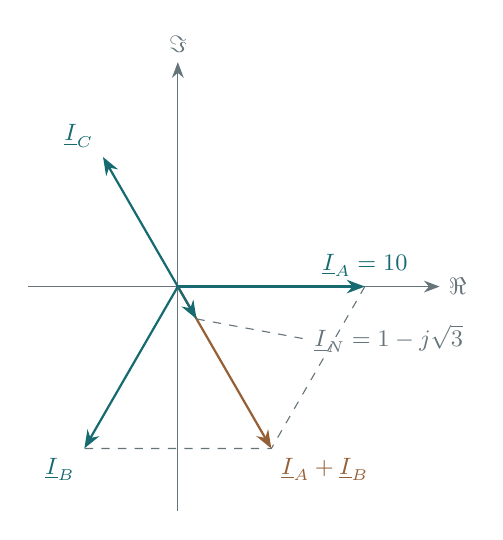
\begin{tikzpicture}[scale=.95,transform shape]
\draw[axis] (-2,0)--(3.5,0) node[right]{$\Re$};\draw[axis] (0,-3)--(0,3) node[above]{$\Im$};
\draw[motion] (0,0)--(2.5,0) node[above]{$\underline I_A=10$};
\draw[motion] (0,0)--(-1.25,-2.165) node[below left]{$\underline I_B$};
\draw[motion] (0,0)--(-1,1.732) node[above left]{$\underline I_C$};
\draw[guide] (2.5,0)--(1.25,-2.165)--(-1.25,-2.165);
\draw[force] (0,0)--(1.25,-2.165) node[below right]{$\underline I_A+\underline I_B$};
\draw[traj,-{Stealth}] (0,0)--(.25,-.433);
\draw[guide] (.25,-.433)--(1.7,-.7) node[right]{$\underline I_N=1-j\sqrt3$};

\end{tikzpicture}
\figcaption{解图电5.6A\quad 接中线时的有效值电流相量}
\end{minipage}\end{center}

解图电5.6B把线电压画成两个相电势端点之间的有向边：
\begin{align*}
 \underline U_{AB}&=\underline E_A-\underline E_B=220\sqrt3\,e^{j\pi/6},\\
 \underline U_{BC}&=\underline E_B-\underline E_C=220\sqrt3\,e^{-j\pi/2},\\
 \underline U_{CA}&=\underline E_C-\underline E_A=220\sqrt3\,e^{j5\pi/6}.
\end{align*}
三者有效值均为$220\sqrt3\simeq381.05\,{\rm V}$，通常约写$380\,{\rm V}$；相位沿用同一个时间原点。

\begin{center}\begin{minipage}{.97\linewidth}\centering
\begin{tikzpicture}[scale=.9,transform shape,font=\small]
\coordinate(O)at(0,0);\coordinate(A)at(3,0);\coordinate(B)at(-1.5,-2.59808);\coordinate(C)at(-1.5,2.59808);
\foreach\p in{A,B,C}{\draw[guide,-{Stealth}](O)--(\p);\fill(\p)circle(.035);}
\draw[motion](B)--(A)node[midway,below right]{$\underline U_{AB}$};
\draw[motion](C)--(B)node[midway,left]{$\underline U_{BC}$};
\draw[motion](A)--(C)node[midway,above right]{$\underline U_{CA}$};
\node[above left]at(O){$O$};\node[right]at(A){$A$};\node[below]at(B){$B$};\node[above]at(C){$C$};
\node[align=left,anchor=west]at(4.2,.6){半径：相电压$220\,\mathrm V$\\边长：线电压$220\sqrt3\,\mathrm V$\\$\underline U_{AB}$由B指向A\\$\arg\underline U_{AB}=30^\circ$\\三条有向边首尾闭合};
\end{tikzpicture}
\figcaption{解图电5.6B　三条线电压是相电势端点之间的有向边。相电压从O指向端点，线电压从被减相的端点指向另一端点。}
\end{minipage}\end{center}

解图电5.6B中，$\underline U_{AB}$与$\underline E_A$夹$30^\circ$。由余弦定理，$|\underline U_{AB}|^2=220^2+220^2-2(220)^2\cos120^\circ=3(220)^2$；其余两边由轮换指标得到。三边有向和为零，对应$\underline U_{AB}+\underline U_{BC}+\underline U_{CA}=0$。三个端点A、B、C由理想电源固定，是否接中线不会改变这个三角形。


中线断开后，电源相电势和线电压不变，但$O'$浮置。由 $O^{\prime}$ 指向各相端点的电压正是三支负载所承受的电压。令$\underline V=V_{O'}-V_O$。解图电5.6C的节点方程为
\[
 \frac{\underline E_A-\underline V}{22}
 +\frac{\underline E_B-\underline V}{22}
 +\frac{\underline E_C-\underline V}{27.5}=0.
\]
所以
\[
 \underline V=\frac{\sum\underline E_k/R_k}{\sum1/R_k}
 =\frac{55}{7}(1-j\sqrt3)\ {\rm V}.
\]
再逐支路相减、除电阻：
\[
 \boxed{\begin{aligned}
 \underline I_A&=\frac{135+j5\sqrt3}{14}\ {\rm A},\\
 \underline I_B&=\frac{-75-j65\sqrt3}{14}\ {\rm A},\\
 \underline I_C&=\frac{-30+j30\sqrt3}{7}\ {\rm A}.
 \end{aligned}}
\]
相应有效值和相位约为
\[
 \underline I_A=9.663\angle3.670^\circ,\quad
 \underline I_B=9.663\angle(-123.670^\circ),\quad
 \underline I_C=8.571\angle120^\circ\quad({\rm A}).
\]
瞬时电流为$\sqrt2|\underline I_k|\cos(\omega t+\arg\underline I_k)$。三个复数相加为零，符合断中线后的电流守恒；它们不再相差严格$120^\circ$。

\begin{center}\begin{minipage}{.98\linewidth}\centering
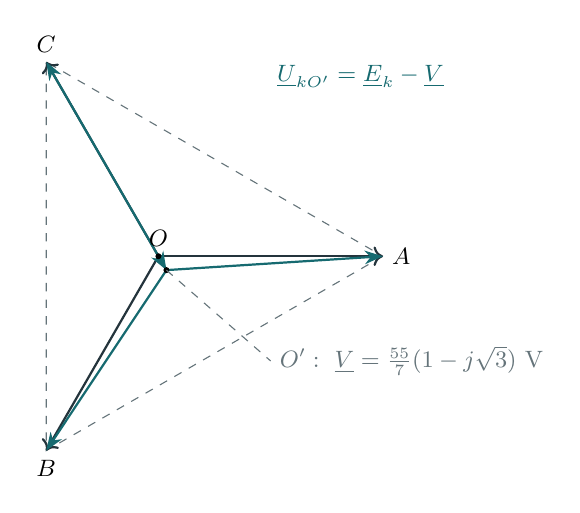
\begin{tikzpicture}[scale=.95,transform shape]

\coordinate (O) at (0,0);\coordinate (N) at (.1071,-.1856);
\coordinate (A) at (3,0);\coordinate (B) at (-1.5,-2.598);\coordinate (C) at (-1.5,2.598);
\draw[guide] (A)--(B)--(C)--cycle;
\foreach \p in {A,B,C}{\draw[object,->] (O)--(\p);\draw[motion] (N)--(\p);}
\draw[traj,-{Stealth}](O)--(N);
\fill (O) circle(.04) (N) circle(.04);
\node[above] at (O){$O$};\node[right] at (A){$A$};
\node[below] at (B){$B$};\node[above] at (C){$C$};
\draw[guide] (N)--(1.5,-1.4) node[right]{$O':\ \underline V=\frac{55}7(1-j\sqrt3)\ {\rm V}$};
\node[text=accent] at (2.7,2.4){$\underline U_{kO'}=\underline E_k-\underline V$};

\end{tikzpicture}
\figcaption{解图电5.6C\quad 断中线后负载电压随中性点漂移，线电压保持不变}
\end{minipage}\end{center}


在解图电5.6C中，沿节点漂移箭头计算其大小和相角。各相导纳之和$G=1/22+1/22+1/27.5=7/55\,\Omega^{-1}$；接中线时流向O的合电流$S=\sum\underline E_k/R_k=(1-\mathrm j\sqrt3)\,\mathrm A$。断中线后必须由同一个节点电势抵消这段电流，所以$\underline V=S/G=(55/7)(1-\mathrm j\sqrt3)\,\mathrm V$，其模$110/7\,\mathrm V$、相角$-60^\circ$。例如A支路
\[
\underline I_A=\frac{220-(55/7)(1-\mathrm j\sqrt3)}{22}
=\frac{135+\mathrm j5\sqrt3}{14}\,\mathrm A,
\]
B、C支路也分别减去同一个$\underline V$，因为三支路汇于同一个 $O^{\prime}$。由此可验$22\underline I_A-22\underline I_B=\underline U_{AB}$、$22\underline I_B-27.5\underline I_C=\underline U_{BC}$，节点法同时满足两条线电压关系。

另一种完整解法直接对图B、C的实际回路列线电压式，并配合浮置星点的电流守恒：
\[
22\underline I_A-22\underline I_B=\underline U_{AB},\qquad
22\underline I_B-27.5\underline I_C=\underline U_{BC},\qquad
\underline I_A+\underline I_B+\underline I_C=0.
\]
用最后一式消去$\underline I_C$，第二式成为$27.5\underline I_A+49.5\underline I_B=\underline U_{BC}$。第一式给$\underline I_A=\underline I_B+\underline U_{AB}/22$，代回得到
\[
\underline I_B=\frac{\underline U_{BC}-(5/4)\underline U_{AB}}{77\,\Omega},\qquad
\underline I_A=\frac{\underline U_{BC}+(9/4)\underline U_{AB}}{77\,\Omega},\qquad
\underline I_C=-\underline I_A-\underline I_B.
\]
这些式子中电压除以电阻才是电流；前面的22、27.5、49.5均代表以欧姆计的实际电阻。把本题同一时间原点下的两个线电压相量代入，就逐项得到框内三个复数；不需要另设中性点未知量。两种方法分别突出节点漂移和回路电压，物理约束完全相同。

若希望以$U_{AB}$的相位作为参照，应将全部相量统一乘$e^{-\mathrm j\pi/6}$。把旋转后的相量记为$\underline J_k$，有
\[
\underline J_A=\left(5\sqrt3-\mathrm j\frac{30}{7}\right)\mathrm A,\quad
\underline J_B=\left(-5\sqrt3-\mathrm j\frac{30}{7}\right)\mathrm A,\quad
\underline J_C=\mathrm j\frac{60}{7}\,\mathrm A.
\]
于是
\[
J_A=J_B=\sqrt{75+\frac{900}{49}}=\frac5{7}\sqrt{183}\,\mathrm A,
\quad J_C=\frac{60}{7}\,\mathrm A,
\quad \cos\phi=\frac7{\sqrt{61}},\quad
\sin\phi=\frac{2\sqrt3}{\sqrt{61}},\quad \phi\simeq26.330^\circ.
\]
令$\vartheta=\omega t+\pi/6$，使线电压写成$u_{AB}=220\sqrt6\cos\vartheta\,\mathrm V$，瞬时电流就是
\[
\begin{aligned}
i_A&=\sqrt2\frac5{7}\sqrt{183}\cos(\vartheta-\phi)\,\mathrm A,\\
i_B&=\sqrt2\frac5{7}\sqrt{183}\cos(\vartheta+\phi+\pi)\,\mathrm A,\\
i_C&=\sqrt2\frac{60}{7}\cos(\vartheta+\pi/2)\,\mathrm A.
\end{aligned}
\]
这与前面相角$3.670^\circ,-123.670^\circ,120^\circ$的三式是同一组电流。两种记法只差共同的参照旋转，瞬时物理量并未改变；有效值前的$\sqrt2$则是从相量到瞬时幅值必需的换算。

按节点电势求各负载电压与总功率。由图C各箭头$\underline U_{kO'}=\underline E_k-\underline V$，A、B负载电压有效值均为$110\sqrt{183}/7\,\mathrm V\simeq212.58\,\mathrm V$，C负载为$1650/7\,\mathrm V\simeq235.71\,\mathrm V$。较大的C相电阻分得更高的电压，因此断中线后仍把三相负载电压一律设220伏会破坏节点守恒。总有功功率为$\sum R_k|\underline I_k|^2=42900/7\,\mathrm W\simeq6128.57\,\mathrm W$，与$\sum\Re(\underline E_k\underline I_k^*)$相同，两种求和分别给出负载吸收和电源送出的有功功率。


\Needspace{13\baselineskip}

\pdfbookmark[2]{第 7 题 非正弦电源的谐波叠加与瞬时投影}{q7}

\section*{第 7 题\quad 非正弦电源的谐波叠加与瞬时投影}\label{q:7}


电源$\mathcal E(t)=4\mathcal E_0\cos^3\omega t$接在一个电阻$R$与并联支路$(R\parallel L)$串联的电路上，且$\omega L=R$。求周期稳态下$t=0$时电感两端的电压。取该电压为图中并联支路左端对右端的电势差。

\begin{center}\begin{minipage}{.98\linewidth}\centering
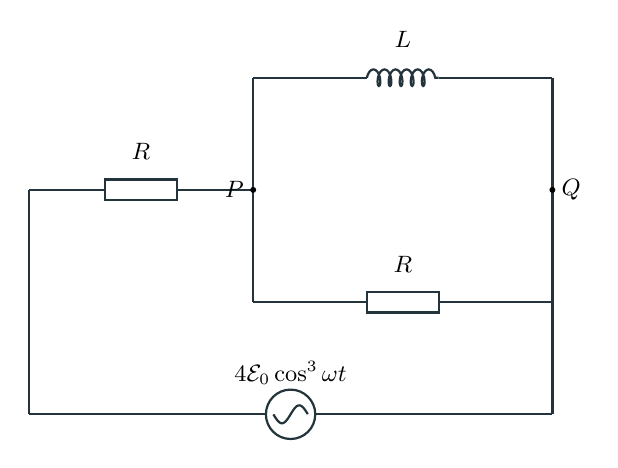
\begin{tikzpicture}[scale=.95,transform shape]
\begin{scope}[shift={(1.5,2.0)},rotate=0.0]\draw[object] (-1.5,0)--(-0.48,0) (0.48,0)--(1.5,0);\draw[object,fill=white] (-.48,-.14) rectangle (.48,.14);\end{scope}\node[anchor=south,fill=white,inner sep=1.5pt] at (1.5000,2.3400) {$R$};
\draw[object] (3,2)--(3,3.5);
\begin{scope}[shift={(5.0,3.5)},rotate=0.0]\draw[object] (-2.0,0)--(-0.48,0) (0.48,0)--(2.0,0);\draw[object,decorate,decoration={coil,aspect=.45,segment length=4pt,amplitude=3pt}] (-.48,0)--(.48,0);\end{scope}\node[anchor=south,fill=white,inner sep=1.5pt] at (5.0000,3.8400) {$L$};
\draw[object] (7,3.5)--(7,2);
\draw[object] (3,2)--(3,0.5);
\begin{scope}[shift={(5.0,0.5)},rotate=0.0]\draw[object] (-2.0,0)--(-0.48,0) (0.48,0)--(2.0,0);\draw[object,fill=white] (-.48,-.14) rectangle (.48,.14);\end{scope}\node[anchor=south,fill=white,inner sep=1.5pt] at (5.0000,0.8400) {$R$};
\draw[object] (7,0.5)--(7,2);
\draw[object] (0,2)--(0,-1);
\draw[object] (7,2)--(7,-1);
\begin{scope}[shift={(3.5,-1.0)},rotate=0.0]\draw[object] (-3.5,0)--(-0.33,0) (0.33,0)--(3.5,0);\draw[object,fill=white] (0,0) circle (.33);\draw[object] plot[domain=-.23:.23,samples=35] (\x,{.12*sin(780*\x)});\end{scope}\node[anchor=south,fill=white,inner sep=1.5pt] at (3.5000,-0.6600) {$4\mathcal E_0\cos^3\omega t$};\fill (3,2) circle(.04);\node[left] at (3,2) {$P$};\fill (7,2) circle(.04);\node[right] at (7,2) {$Q$};
\end{tikzpicture}
\figcaption{图电5.7\quad 串联电阻及$R\parallel L$并联支路}
\end{minipage}\end{center}

\Needspace{6\baselineskip}\subsection*{解答}


先按图电5.7统一端口和电压正向。三倍角公式给
\[
 \mathcal E(t)=3\mathcal E_0\cos\omega t+\mathcal E_0\cos3\omega t.
\]
线性电路允许对两个频率分别求解，再叠加瞬时实数。基波箭头以 $\omega$ 转动，三次谐波箭头以 $3\omega$ 转动；任一时刻将两条实轴投影相加。
把图电5.7中串联电阻电流记为$i$，并联电阻支流记为$i_R$，电感支流为$i_L$，均取由左到右为正。实际电路同时满足
\[
Ri+Ri_R=\mathcal E_1(t)+\mathcal E_3(t),\qquad
Ri_R-L\dot i_L=0,\qquad i-i_R-i_L=0.
\]
三式均线性，因此可把两个频率的电压分别施加到同一电路，求出两组支路电流和电压，再逐时刻相加。同一电感在两种频率下的电抗分别为$\omega L=R$和$3\omega L=3R$。以下复相量与题设$\mathcal E_0$均取余弦的峰值幅度；换算有效值时才将峰值除以$\sqrt2$。


\begin{center}\begin{minipage}{.98\linewidth}\centering
\begin{tikzpicture}[scale=.92,transform shape]

\begin{scope}
\draw[axis] (0,0)--(4.5,0) node[right]{$\Re$};\draw[axis] (0,0)--(0,2.6) node[above]{$\Im$};
\draw[motion] (0,0)--(3.6,1.8) node[above]{$\underline U_{L,1}$};
\draw[guide] (3.6,1.8)--(3.6,0);\node[below] at (2.6,-.1){$\Re U_{L,1}=6\mathcal E_0/5$};
\node at (2,3.1){基波：角速度$\omega$};
\end{scope}
\begin{scope}[shift={(7,0)}]
\draw[axis] (0,0)--(4.4,0) node[right]{$\Re$};\draw[axis] (0,0)--(0,2.6) node[above]{$\Im$};
\draw[force] (0,0)--(1.4595,.2432);
\draw[guide] (1.4595,.2432)--(1.4595,0);
\node[above right] at (1.4595,.2432){$\underline U_{L,3}$};
\node[below] at (2.3,-.1){$\Re U_{L,3}=18\mathcal E_0/37$};
\node at (2,3.1){三次谐波：角速度$3\omega$};
\end{scope}

\end{tikzpicture}
\figcaption{解图电5.7A\quad $t=0$取各谐波的实轴投影后相加}
\end{minipage}\end{center}

解图电5.7A中，令某一谐波角频率为$\Omega$、$x=\Omega L/R$，则并联阻抗
\[
 Z_p=\frac{j\Omega LR}{R+j\Omega L},\qquad
 H(\Omega)=\frac{\underline U_L}{\underline{\mathcal E}}
 =\frac{Z_p}{R+Z_p}
 =\frac{jx}{1+2jx}
 =\frac{2x^2+jx}{1+4x^2}.
\]
基波$x=1$，三次谐波$x=3$，因此
\[
 \underline U_{L,1}=3\mathcal E_0\frac{2+j}{5},\qquad
 \underline U_{L,3}=\mathcal E_0\frac{18+3j}{37}.
\]
它们均采用余弦约定，实际电压为
\[
 u_L(t)=\mathcal E_0\left[
 \frac65\cos\omega t-\frac35\sin\omega t
 +\frac{18}{37}\cos3\omega t-\frac3{37}\sin3\omega t\right].
\]
在$t=0$，虚部对应的正弦项均为零，所求为
\[
 \boxed{u_L(0)=\left(\frac65+\frac{18}{37}\right)\mathcal E_0
 =\frac{312}{185}\mathcal E_0
 \simeq1.68649\,\mathcal E_0.}
\]
解图电5.7A中两根谐波箭头在$t=0$的横轴投影分别为$6\mathcal E_0/5$和$18\mathcal E_0/37$，这才是两个瞬时电压。两箭头都按本身的源幅值作图，因此两个投影中的基波项已经含源幅值的因子3。

时域方程直接连接总电流与电感支流。取$i_L$从左流向右，并联电阻电流为$u_L/R$，两支相加得总电流$i_L+u_L/R$，所以
\[
 \mathcal E=R i_L+2u_L,\qquad u_L=L\dot i_L,
\]
即$2L\dot i_L+Ri_L=\mathcal E$，其稳态传递关系与上式一致。若回路刚接通，还可叠加$A e^{-Rt/(2L)}$的电流，其电压也会影响$t=0$；本题因此明确取周期稳态。


下面把解图电5.7B、C的支流相量接到电压多边形上，说明两个频率的超前角怎样形成。为避免与时域谐波下标混淆，以下以$n=1,3$标谐波，$U_n$表示该次谐波的并联电压幅值；作几何图时暂把$\underline U_n$放在实轴，而把对应电源幅值记为$E_1=3\mathcal E_0$、$E_3=\mathcal E_0$。这两个局部参照只是分别旋转了各自的单频图，最终还要转回两个电源共同的$t=0$参照。

先看基波。并联电阻支流与$\underline U_1$同相，电感支流滞后$90^\circ$且等幅，因此
\[
I_{R,1}=\frac{U_1}{R},\qquad I_{L,1}=\frac{U_1}{\omega L}=I_{R,1},\qquad
I_1=\sqrt2I_{R,1},\qquad RI_1=\sqrt2U_1.
\]
\begin{center}\begin{minipage}{.97\linewidth}\centering
\begin{tikzpicture}[font=\small]
\begin{scope}
\draw[guide](-.2,0)--(2,0)(0,.25)--(0,-1.7);
\draw[motion](0,0)--(1.4,0)node[above]{$\underline I_{R,n}$};
\draw[force](0,0)--(0,-1.400000)node[left]{$\underline I_{L,n}$};
\draw[traj,-{Stealth}](0,0)--(1.4,-1.400000)node[below right]{$\underline I_n$};
\draw[guide](1.4,0)--(1.4,-1.400000)--(0,-1.400000);
\node[above]at(.8,.65){电流以$U_n/R$为单位};
\end{scope}
\begin{scope}[shift={(4.4,0)}]
\draw[guide](-.2,0)--(3.2,0);
\draw[motion](0,0)--(1.4,0)node[midway,above]{$\underline U_n$};
\draw[force](1.4,0)--(2.8,-1.400000)node[midway,above right]{$R\underline I_n$};
\draw[traj,-{Stealth}](0,0)--(2.8,-1.400000)node[below right]{$\underline{\mathcal E}_n$};
\draw[guide](2.8,-1.400000)--(2.8,0);
\node[above]at(1.4,.65){电压以$U_n$为单位};
\end{scope}
\node[align=left,anchor=west]at(8.1,-.3){本图以并联电压为实轴\\$\underline{\mathcal E}_n/U_n=2-\mathrm j/1$\\源电压向下偏转\\换回源相位参照时\\并联电压超前源电压};
\end{tikzpicture}
\figcaption{解图电5.7B　基波先合电流、再将串联电阻电压首尾接在并联电压后。电流图和电压图分别归一化，分别用该频率的电流幅值与电压幅值定标。}
\end{minipage}\end{center}

解图电5.7B左图合电流的水平分量为$U_1/R$，竖直分量为$-U_1/R$；串联电阻压降$R\underline I_1$与合电流同相，故右图中它的水平、竖直分量分别是$U_1,-U_1$。再加并联电压$\underline U_1$，电源相量成为$2U_1-\mathrm jU_1$。由此
\[
E_1=\sqrt5U_1,\quad \cos\phi_1=\frac2{\sqrt5},\quad
\sin\phi_1=\frac1{\sqrt5},\quad
U_1\cos\phi_1=\frac25E_1,\quad
U_1\sin\phi_1=\frac15E_1.
\]
电源在局部图中向下偏转，而并联电压在电源相位参照中超前$\phi_1$，所以换回实轴后，$\underline U_{L,1}=(2+\mathrm j)E_1/5$，不是取负的虚部。将$E_1=3\mathcal E_0$代回，恰为前面的$3(2+\mathrm j)\mathcal E_0/5$。

再看三次谐波，电感电抗变为$3R$，并联支流和合电流满足
\[
I_{R,3}=\frac{U_3}{R},\quad I_{L,3}=\frac13I_{R,3},\quad
I_3=\frac{\sqrt{10}}3I_{R,3},\quad
RI_3=\frac{\sqrt{10}}3U_3.
\]
\begin{center}\begin{minipage}{.97\linewidth}\centering
\begin{tikzpicture}[font=\small]
\begin{scope}
\draw[guide](-.2,0)--(2,0)(0,.25)--(0,-1.7);
\draw[motion](0,0)--(1.4,0)node[above]{$\underline I_{R,n}$};
\draw[force](0,0)--(0,-0.466667)node[left]{$\underline I_{L,n}$};
\draw[traj,-{Stealth}](0,0)--(1.4,-0.466667)node[below right]{$\underline I_n$};
\draw[guide](1.4,0)--(1.4,-0.466667)--(0,-0.466667);
\node[above]at(.8,.65){电流以$U_n/R$为单位};
\end{scope}
\begin{scope}[shift={(4.4,0)}]
\draw[guide](-.2,0)--(3.2,0);
\draw[motion](0,0)--(1.4,0)node[midway,above]{$\underline U_n$};
\draw[force](1.4,0)--(2.8,-0.466667)node[midway,above right]{$R\underline I_n$};
\draw[traj,-{Stealth}](0,0)--(2.8,-0.466667)node[below right]{$\underline{\mathcal E}_n$};
\draw[guide](2.8,-0.466667)--(2.8,0);
\node[above]at(1.4,.65){电压以$U_n$为单位};
\end{scope}
\node[align=left,anchor=west]at(8.1,-.3){本图以并联电压为实轴\\$\underline{\mathcal E}_n/U_n=2-\mathrm j/3$\\源电压向下偏转\\换回源相位参照时\\并联电压超前源电压};
\end{tikzpicture}
\figcaption{解图电5.7C　三次谐波电感支流缩为电阻支流的三分之一。右图的电源竖直分量也为并联电压的负三分之一。}
\end{minipage}\end{center}

解图电5.7C中，串联电阻电压的水平分量仍为$U_3$，向下分量却只有$U_3/3$。电源相量于是为$2U_3-\mathrm jU_3/3$，所以
\[
E_3=\frac{\sqrt{37}}3U_3,\qquad
\cos\phi_3=\frac6{\sqrt{37}},\qquad \sin\phi_3=\frac1{\sqrt{37}}.
\]
再投影到电源的方向及其超前$90^\circ$方向，得到
\[
U_3\cos\phi_3=\frac3{\sqrt{37}}E_3\frac6{\sqrt{37}}=\frac{18}{37}E_3,
\qquad
U_3\sin\phi_3=\frac3{\sqrt{37}}E_3\frac1{\sqrt{37}}=\frac3{37}E_3.
\]
这正是$\underline U_{L,3}=(18+3\mathrm j)E_3/37$的两个分量，三次谐波的电流比例、电压多边形、模和相位全部进入了计算。

回到解图电5.7A，两个电源在$t=0$均沿同一实轴，故两个输出箭头的横向投影可直接相加；但每个横、竖分量都要保留对应电源的幅值。于是同一时刻的几何分量为
\[
U_{\parallel}(0)=\left(\frac25\cdot3+\frac{18}{37}\right)\mathcal E_0
=\frac{312}{185}\mathcal E_0,
\qquad
U_{\perp}(0)=\left(\frac15\cdot3+\frac3{37}\right)\mathcal E_0
=\frac{126}{185}\mathcal E_0.
\]
只有前一项是$t=0$的实际电压。后一项是同一时刻箭头在虚轴上的几何投影；实际电压由实轴投影给出。随着时间推进，基波和三次谐波分别旋转$\omega t$和$3\omega t$，相对夹角会变化，因此应逐时刻投影求和。

解图B、C中两个频率的电感稳态电流相加，得到时域解：
\[
i_{L,\mathrm s}(t)=\frac{\mathcal E_0}{R}
\left[\frac35\cos\omega t+\frac65\sin\omega t
+\frac1{37}\cos3\omega t+\frac6{37}\sin3\omega t\right].
\]
逐项求导并用$\omega L=R$，$L\dot i_{L,\mathrm s}$就是前面的$u_L(t)$；代入$2L\dot i_L+Ri_L=\mathcal E$也逐项成立。若改成零电流接通，则应另加$-[116\mathcal E_0/(185R)]e^{-Rt/(2L)}$的电感电流，输出多出$[58\mathcal E_0/185]e^{-Rt/(2L)}$，从而接通瞬间$u_L(0^+)=2\mathcal E_0$。这个数值适用于零初始电流启动；本题的$312\mathcal E_0/185$适用于周期稳态，二者初始条件不同。


\Needspace{13\baselineskip}

\pdfbookmark[2]{第 8 题 含电抗桥支路的复阻抗网络}{q8}

\section*{第 8 题\quad 含电抗桥支路的复阻抗网络}\label{q:8}


图中交流网络含三只电阻$R$、两只电感$L$、两只电容$C$。端口$A,B$间加$u=U_0\cos(\omega t+\varphi_u)$，且$\omega L=1/(\omega C)=R$。$A\to Y$臂为$R,L$串联，$Y\to B$臂为$C$；$A\to X$臂为$C$，$X\to B$臂为$L,R$串联，$X,Y$间跨接第三只$R$。用复数法求端口阻抗的模，以及中间电阻电流的有效值。

\begin{center}\begin{minipage}{.98\linewidth}\centering
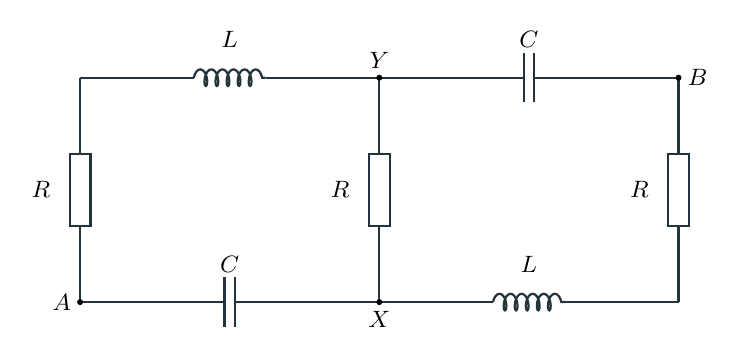
\begin{tikzpicture}[scale=.95,transform shape]
\begin{scope}[shift={(0.0,1.5)},rotate=90.0]\draw[object] (-1.5,0)--(-0.48,0) (0.48,0)--(1.5,0);\draw[object,fill=white] (-.48,-.14) rectangle (.48,.14);\end{scope}\node[anchor=east,fill=white,inner sep=1.5pt] at (-0.3400,1.5000) {$R$};
\begin{scope}[shift={(2.0,3.0)},rotate=0.0]\draw[object] (-2.0,0)--(-0.48,0) (0.48,0)--(2.0,0);\draw[object,decorate,decoration={coil,aspect=.45,segment length=4pt,amplitude=3pt}] (-.48,0)--(.48,0);\end{scope}\node[anchor=south,fill=white,inner sep=1.5pt] at (2.0000,3.3400) {$L$};
\begin{scope}[shift={(6.0,3.0)},rotate=0.0]\draw[object] (-2.0,0)--(-0.22,0) (0.22,0)--(2.0,0);\draw[object] (-.07,-.33)--(-.07,.33) (.07,-.33)--(.07,.33) (-.22,0)--(-.07,0) (.07,0)--(.22,0);\end{scope}\node[anchor=south,fill=white,inner sep=1.5pt] at (6.0000,3.3400) {$C$};
\begin{scope}[shift={(2.0,0.0)},rotate=0.0]\draw[object] (-2.0,0)--(-0.22,0) (0.22,0)--(2.0,0);\draw[object] (-.07,-.33)--(-.07,.33) (.07,-.33)--(.07,.33) (-.22,0)--(-.07,0) (.07,0)--(.22,0);\end{scope}\node[anchor=south,fill=white,inner sep=1.5pt] at (2.0000,0.3400) {$C$};
\begin{scope}[shift={(6.0,0.0)},rotate=0.0]\draw[object] (-2.0,0)--(-0.48,0) (0.48,0)--(2.0,0);\draw[object,decorate,decoration={coil,aspect=.45,segment length=4pt,amplitude=3pt}] (-.48,0)--(.48,0);\end{scope}\node[anchor=south,fill=white,inner sep=1.5pt] at (6.0000,0.3400) {$L$};
\begin{scope}[shift={(8.0,1.5)},rotate=90.0]\draw[object] (-1.5,0)--(-0.48,0) (0.48,0)--(1.5,0);\draw[object,fill=white] (-.48,-.14) rectangle (.48,.14);\end{scope}\node[anchor=east,fill=white,inner sep=1.5pt] at (7.6600,1.5000) {$R$};
\begin{scope}[shift={(4.0,1.5)},rotate=90.0]\draw[object] (-1.5,0)--(-0.48,0) (0.48,0)--(1.5,0);\draw[object,fill=white] (-.48,-.14) rectangle (.48,.14);\end{scope}\node[anchor=east,fill=white,inner sep=1.5pt] at (3.6600,1.5000) {$R$};\fill (0,0) circle(.04);\node[left] at (0,0) {$A$};\fill (8,3) circle(.04);\node[right] at (8,3) {$B$};\fill (4,0) circle(.04);\node[below] at (4,0) {$X$};\fill (4,3) circle(.04);\node[above] at (4,3) {$Y$};
\end{tikzpicture}
\figcaption{图电5.8\quad 不能删去中间电阻的交流桥}
\end{minipage}\end{center}

\Needspace{6\baselineskip}\subsection*{解答}


图电5.8中电抗分别为$Z_L=jR,\ Z_C=-jR$。令总电流$\underline I$从$A$流入，$\underline I_1$沿$A\to Y$，桥电流$\underline I_2$沿$X\to Y$；于是$A\to X$电流为$\underline I-\underline I_1$，$Y\to B$为$\underline I_1+\underline I_2$，$X\to B$为$\underline I-\underline I_1-\underline I_2$。

\begin{center}\begin{minipage}{.98\linewidth}\centering
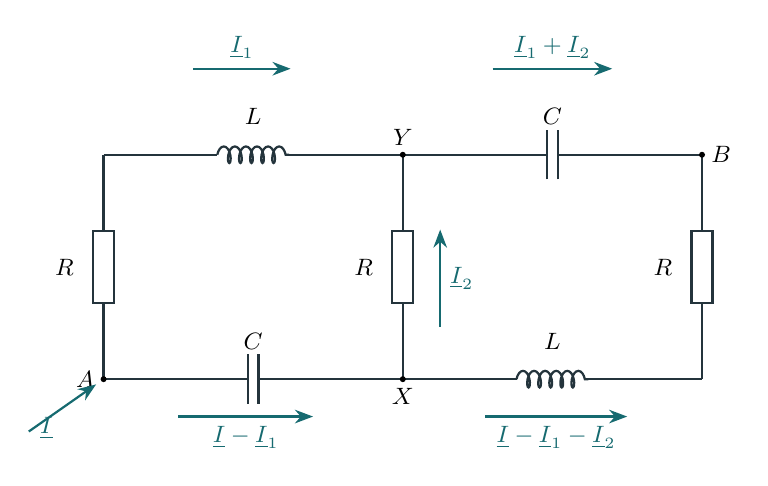
\begin{tikzpicture}[scale=.95,transform shape]
\begin{scope}[shift={(0.0,1.5)},rotate=90.0]\draw[object] (-1.5,0)--(-0.48,0) (0.48,0)--(1.5,0);\draw[object,fill=white] (-.48,-.14) rectangle (.48,.14);\end{scope}\node[anchor=east,fill=white,inner sep=1.5pt] at (-0.3400,1.5000) {$R$};
\begin{scope}[shift={(2.0,3.0)},rotate=0.0]\draw[object] (-2.0,0)--(-0.48,0) (0.48,0)--(2.0,0);\draw[object,decorate,decoration={coil,aspect=.45,segment length=4pt,amplitude=3pt}] (-.48,0)--(.48,0);\end{scope}\node[anchor=south,fill=white,inner sep=1.5pt] at (2.0000,3.3400) {$L$};
\begin{scope}[shift={(6.0,3.0)},rotate=0.0]\draw[object] (-2.0,0)--(-0.22,0) (0.22,0)--(2.0,0);\draw[object] (-.07,-.33)--(-.07,.33) (.07,-.33)--(.07,.33) (-.22,0)--(-.07,0) (.07,0)--(.22,0);\end{scope}\node[anchor=south,fill=white,inner sep=1.5pt] at (6.0000,3.3400) {$C$};
\begin{scope}[shift={(2.0,0.0)},rotate=0.0]\draw[object] (-2.0,0)--(-0.22,0) (0.22,0)--(2.0,0);\draw[object] (-.07,-.33)--(-.07,.33) (.07,-.33)--(.07,.33) (-.22,0)--(-.07,0) (.07,0)--(.22,0);\end{scope}\node[anchor=south,fill=white,inner sep=1.5pt] at (2.0000,0.3400) {$C$};
\begin{scope}[shift={(6.0,0.0)},rotate=0.0]\draw[object] (-2.0,0)--(-0.48,0) (0.48,0)--(2.0,0);\draw[object,decorate,decoration={coil,aspect=.45,segment length=4pt,amplitude=3pt}] (-.48,0)--(.48,0);\end{scope}\node[anchor=south,fill=white,inner sep=1.5pt] at (6.0000,0.3400) {$L$};
\begin{scope}[shift={(8.0,1.5)},rotate=90.0]\draw[object] (-1.5,0)--(-0.48,0) (0.48,0)--(1.5,0);\draw[object,fill=white] (-.48,-.14) rectangle (.48,.14);\end{scope}\node[anchor=east,fill=white,inner sep=1.5pt] at (7.6600,1.5000) {$R$};
\begin{scope}[shift={(4.0,1.5)},rotate=90.0]\draw[object] (-1.5,0)--(-0.48,0) (0.48,0)--(1.5,0);\draw[object,fill=white] (-.48,-.14) rectangle (.48,.14);\end{scope}\node[anchor=east,fill=white,inner sep=1.5pt] at (3.6600,1.5000) {$R$};\fill (0,0) circle(.04);\node[left] at (0,0) {$A$};\fill (8,3) circle(.04);\node[right] at (8,3) {$B$};\fill (4,0) circle(.04);\node[below] at (4,0) {$X$};\fill (4,3) circle(.04);\node[above] at (4,3) {$Y$};
\draw[motion] (-1,-.7)--(-.1,-.07) node[midway,below left]{$\underline I$};
\draw[motion] (1.2,4.15)--(2.5,4.15) node[midway,above]{$\underline I_1$};
\draw[motion] (4.5,.7)--(4.5,2) node[midway,right]{$\underline I_2$};
\draw[motion] (5.2,4.15)--(6.8,4.15) node[midway,above]{$\underline I_1+\underline I_2$};
\draw[motion] (1,-.5)--(2.8,-.5) node[midway,below]{$\underline I-\underline I_1$};
\draw[motion] (5.1,-.5)--(7,-.5) node[midway,below]{$\underline I-\underline I_1-\underline I_2$};

\end{tikzpicture}
\figcaption{解图电5.8A\quad 先用节点守恒统一五条支路电流}
\end{minipage}\end{center}

解图电5.8A标出这五个电流。比较$A\to Y$两条路径和$X\to B$两条路径的压降：
\begin{align*}
 (1+j)R\underline I_1&=-jR(\underline I-\underline I_1)+R\underline I_2,\\
 R\underline I_2-jR(\underline I_1+\underline I_2)
 &=(1+j)R(\underline I-\underline I_1-\underline I_2).
\end{align*}
约去$R$整理为
\[
 \underline I_2=\underline I_1+j\underline I,\qquad
 2\underline I_2=(1+j)\underline I-\underline I_1.
\]
解得
\[
 \underline I_1=\frac{1-j}{3}\underline I,\qquad
 \underline I_2=\frac{1+2j}{3}\underline I .
\]
沿$A\to Y\to B$求端口电压：
\begin{align*}
 \underline U&=(1+j)R\underline I_1
 -jR(\underline I_1+\underline I_2)
 =R\underline I_1-jR\underline I_2\\
 &=\frac{3-2j}{3}R\underline I .
\end{align*}
因此
\[
 \boxed{Z_{AB}=\frac{3-2j}{3}R,\qquad
 |Z_{AB}|=\frac{\sqrt{13}}3R.}
\]
网络总体呈容性，阻抗辐角为$-\arctan(2/3)$。用输入峰值相量$\underline U=U_0e^{j\varphi_u}$，
\[
 \underline I_2=\frac{1+2j}{(3-2j)R}\underline U
 =\frac{-1+8j}{13R}\underline U .
\]
桥电流的峰值为$\sqrt{65}\,U_0/(13R)$，故
\[
 \boxed{I_{XY,{\rm rms}}=\sqrt{\frac5{26}}\frac{U_0}{R}
 \simeq0.43853\,\frac{U_0}{R}.}
\]
求平均有功功率时取有效值相量，将总电流有效值记为$I_{\rm rms}$。
解图电5.8A中三只电阻的电流模分别为
$\sqrt2 I_{\rm rms}/3$、$\sqrt2 I_{\rm rms}/3$、
$\sqrt5 I_{\rm rms}/3$，故
\[
P_R=R\left(\frac29+\frac29+\frac59\right)I_{\rm rms}^2
=RI_{\rm rms}^2.
\]
理想电感和电容的平均有功功率为零，输入也应满足
$P_{\rm in}=\operatorname{Re}Z_{AB}\,I_{\rm rms}^2=RI_{\rm rms}^2$。
各电阻的耗散功率相加，等于总电流有效值的平方乘端口阻抗实部。桥臂电阻的功率已计入各电阻的和。

桥电流不为零。两条外臂虽然形状对称，因$L,C$相反的电抗而不平衡。中间支路方向若改为$Y\to X$，复电流整体变号，有效值不变。


上面的相量计算还应展开相位和有效值的最后一步。对桥流分母乘共轭，
\[
\frac{1+2\mathrm j}{3-2\mathrm j}
=\frac{(1+2\mathrm j)(3+2\mathrm j)}{13}
=\frac{-1+8\mathrm j}{13}.
\]
该系数实部负、虚部正，桥流超前端口电压的角为$\psi=\pi-\arctan8\simeq97.125^\circ$，这个角落在第二象限。按同一电流方向写瞬时式：
\[
i_2(t)=\frac{\sqrt{65}\,U_0}{13R}\cos(\omega t+\varphi_u+\psi),
\qquad I_{2,\mathrm{rms}}=\frac{\sqrt{65}\,U_0}{13\sqrt2R}.
\]
有效值不依赖初相$\varphi_u$；桥流参考方向反转只使全部瞬时值变号、相位加$\pi$，不改变此模。

也可以从桥臂两端的节点电势直接求出桥流。取$V_B=0$、$V_A=\underline U$，写$x=V_X/\underline U,y=V_Y/\underline U$，按节点电流守恒有
\[
\frac{x-1}{-\mathrm j}+\frac{x}{1+\mathrm j}+x-y=0,\qquad
\frac{y-1}{1+\mathrm j}+\frac{y}{-\mathrm j}+y-x=0.
\]
这两式分别将图A中从X、Y流出的三支电流相加为零。整理并相加、相减，得到
\[
\frac{3+\mathrm j}{2}x-y=\mathrm j,\qquad
\frac{3+\mathrm j}{2}y-x=\frac{1-\mathrm j}{2},\qquad
x+y=1,\quad x-y=\frac{-1+8\mathrm j}{13}.
\]
所以$x=(6+4\mathrm j)/13$、$y=(7-4\mathrm j)/13$，两点不等势。桥流仍为$(V_X-V_Y)/R=(-1+8\mathrm j)\underline U/(13R)$。
\begin{center}\begin{minipage}{.97\linewidth}\centering
\begin{tikzpicture}[scale=.95,transform shape,font=\small]
\coordinate(B)at(0,0);\coordinate(A)at(4,0);\coordinate(X)at(1.846154,1.230769);\coordinate(Y)at(2.153846,-1.230769);
\draw[axis](-.3,0)--(4.7,0)node[right]{$\Re$};\draw[axis](0,-1.7)--(0,1.8)node[above]{$\Im$};
\draw[motion](B)--(X);\draw[motion](B)--(Y);\draw[guide](B)--(A);
\draw[force](Y)--(X)node[midway,right,fill=white,inner sep=1pt]{$R\underline I_2$};
\foreach\p in{A,B,X,Y}{\fill(\p)circle(.035);}
\node[below left]at(B){$B:0$};\node[above]at(A){$A:1$};\node[above left]at(X){$X$};\node[below right]at(Y){$Y$};
\node[align=left,anchor=west]at(5.7,.3){$\varphi_u=0$，电势除以$U_0$\\$V_X/U_0=(6+4\mathrm j)/13$\\$V_Y/U_0=(7-4\mathrm j)/13$\\电压差箭头由Y端点指向X端点\\桥流正向在实际电路取$X\to Y$};
\end{tikzpicture}
\figcaption{解图电5.8B　两个桥节点的复电势。相量平面中，从Y的端点指向X的端点得到桥臂电压差；电路中的桥流以从X流向Y为正。}
\end{minipage}\end{center}

解图电5.8B按输入相位零画出$x,y$。两点的实部相加为1，虚部等大反号且均非零，因此两点在相量平面上分开。图B中从Y的端点指向X的箭头给出桥臂压差；实际电路以X到Y为桥流正方向，满足$V_X-V_Y=R\underline I_2$。

从这两个节点电势反算各条真实支流，全部保留输入相量的共同因子：
\[
\begin{aligned}
\underline I_1=\underline I_{XB}&=\frac{5-\mathrm j}{13R}\underline U,\\
\underline I_{AX}=\underline I_{YB}&=\frac{4+7\mathrm j}{13R}\underline U,\\
\underline I_2&=\frac{-1+8\mathrm j}{13R}\underline U,\qquad
\underline I=\frac{9+6\mathrm j}{13R}\underline U.
\end{aligned}
\]
例如$Y\to B$是电容支路，$\underline I_{YB}=V_Y/(-\mathrm jR)=(4+7\mathrm j)\underline U/(13R)$；$X\to B$则经串联RL，$\underline I_{XB}=V_X/[(1+\mathrm j)R]=(5-\mathrm j)\underline U/(13R)$。这里相等的是AX与YB的电流相量。桥流等于X点的流入与向B流出的相量差，仍由上式的非零压差给出。
\begin{center}\begin{minipage}{.97\linewidth}\centering
\begin{tikzpicture}[x=.25cm,y=.25cm,font=\small]
\begin{scope}
\draw[axis](-2,0)--(7,0);\draw[axis](0,-2)--(0,9.6);
\draw[motion](0,0)--(5,-1)node[below right]{$I_1$};
\draw[force](0,0)--(-1,8)node[above left]{$I_2$};
\draw[traj,-{Stealth}](0,0)--(4,7)node[right]{$I_{YB}$};
\draw[guide](5,-1)--(4,7)--(-1,8);
\node[above]at(2.2,11){Y节点：$I_1+I_2=I_{YB}$};
\end{scope}
\begin{scope}[shift={(17,0)}]
\draw[axis](-1.2,0)--(11,0);\draw[axis](0,-2)--(0,9.6);
\draw[motion](0,0)--(5,-1)node[below right]{$I_1$};
\draw[force](0,0)--(4,7)node[above left]{$I_{AX}$};
\draw[traj,-{Stealth}](0,0)--(9,6)node[right]{$I$};
\draw[guide](5,-1)--(9,6)--(4,7);
\node[above]at(4,11){A节点：$I_1+I_{AX}=I$};
\end{scope}
\node[below,align=center]at(13,-4){取$\varphi_u=0$，全部电流以$U_0/(13R)$为单位\\两面板横、纵方向均采用相同标度};
\end{tikzpicture}
\figcaption{解图电5.8C　按真实复系数画出的两组节点电流和。所有箭头采用同一峰值尺度，Y节点和A节点的平行四边形分别闭合。}
\end{minipage}\end{center}

解图电5.8C左图的$(5,-1)+(-1,8)=(4,7)$把流入Y的两支电流相加，得到流向B的电流。右图的$(5,-1)+(4,7)=(9,6)$将A点流出的两支相加，得到输入电流。X点流入减去桥流为$(4,7)-(-1,8)=(5,-1)$，余下的流向B。用输入电压相量除以输入电流相量，得到端口复阻抗$\underline U/\underline I=13R/(9+6\mathrm j)=(3-2\mathrm j)R/3$。

若只需求桥流，可先摘开中心电阻，求X、Y之间的戴维南等效。A、B间的两条外路均为总阻抗R的串联支路。此时$V_X^{(0)}=(1+\mathrm j)\underline U$、$V_Y^{(0)}=-\mathrm j\underline U$，开路差压$U_{XY}^{(0)}=(1+2\mathrm j)\underline U$。将理想电压源短接，X和Y各经$(1+\mathrm j)R$与$-\mathrm jR$并联接至同一公共点，每组并联阻抗为$(1-\mathrm j)R$，两组对X、Y串联，因此
\[
Z_{\mathrm{th}}=2(1-\mathrm j)R,\qquad
\underline I_2=\frac{U_{XY}^{(0)}}{R+Z_{\mathrm{th}}}
=\frac{1+2\mathrm j}{(3-2\mathrm j)R}\underline U.
\]
戴维南法与两回路法、节点法一致。这里“摘开”只用于计算中心端口的等效电源，最后已将中心R接回；摘开时测得的 $R/2$ 属于无桥臂的外部网络，接回中心电阻后端口阻抗为前面所得的 $R(3-2\mathrm j)/3$。


\Needspace{13\baselineskip}

\pdfbookmark[2]{第 9 题 有损线圈的等效模型与导纳电桥}{q9}

\section*{第 9 题\quad 有损线圈的等效模型与导纳电桥}\label{q:9}


线圈的品质因数定义为感性无功功率与有功损耗之比$Q=P_{\rm q}/P_{\rm a}$。
\begin{enumerate}
\item 在给定角频率$\omega$下，同一线圈既可描述为$R,L$串联，也可描述为$R',L'$并联，求两组参数关系，并验证$Q$相同。
\item 用图中导纳电桥测线圈。两个比率臂是同一变压器有抽头的副绕组，匝数为$N_1,N_2$、电势同相；另两个臂为可调电阻$R_b$及电容$C$与待测线圈的并联组合，检流计跨接两中点。证明平衡时
$Q=(N_2/N_1)\omega C R_b$。
\end{enumerate}

\begin{center}\begin{minipage}{.98\linewidth}\centering
\begin{tikzpicture}[scale=.9,transform shape]
\begin{scope}[shift={(1.5,1.0)},rotate=0.0]\draw[object] (-1.5,0)--(-0.48,0) (0.48,0)--(1.5,0);\draw[object,fill=white] (-.48,-.14) rectangle (.48,.14);\end{scope}\node[anchor=south,fill=white,inner sep=1.5pt] at (1.5000,1.3400) {$R$};
\begin{scope}[shift={(4.5,1.0)},rotate=0.0]\draw[object] (-1.5,0)--(-0.48,0) (0.48,0)--(1.5,0);\draw[object,decorate,decoration={coil,aspect=.45,segment length=4pt,amplitude=3pt}] (-.48,0)--(.48,0);\end{scope}\node[anchor=south,fill=white,inner sep=1.5pt] at (4.5000,1.3400) {$L$};\node at (3,2.3){串联描述};\draw[object] (8,1)--(8,2);
\begin{scope}[shift={(10.0,2.0)},rotate=0.0]\draw[object] (-2.0,0)--(-0.48,0) (0.48,0)--(2.0,0);\draw[object,decorate,decoration={coil,aspect=.45,segment length=4pt,amplitude=3pt}] (-.48,0)--(.48,0);\end{scope}\node[anchor=south,fill=white,inner sep=1.5pt] at (10.0000,2.3400) {$L'$};
\draw[object] (12,2)--(12,1);
\draw[object] (8,1)--(8,0);
\begin{scope}[shift={(10.0,0.0)},rotate=0.0]\draw[object] (-2.0,0)--(-0.48,0) (0.48,0)--(2.0,0);\draw[object,fill=white] (-.48,-.14) rectangle (.48,.14);\end{scope}\node[anchor=south,fill=white,inner sep=1.5pt] at (10.0000,0.3400) {$R'$};
\draw[object] (12,0)--(12,1);\node at (10,3.1){并联描述};\draw[object] (7.3,1)--(8,1) (12,1)--(12.7,1);\foreach \x in {0,6}{\filldraw[fill=white](\x,1)circle(2pt);}\foreach \x in {7.3,12.7}{\filldraw[fill=white](\x,1)circle(2pt);}
\end{tikzpicture}
\figcaption{图电5.9\quad 串联与并联模型均从两个空心端口接入；在同一测量频率下比较端口阻抗。}
\end{minipage}\end{center}

\Needspace{6\baselineskip}\subsection*{解答}


图电5.9中两种模型必须具有相同的复阻抗。对串联模型$Z=R+j\omega L$，取倒数
\[
 Y=\frac{R}{R^2+\omega^2L^2}
 -j\frac{\omega L}{R^2+\omega^2L^2}.
\]
与并联模型$Y=1/R'-j/(\omega L')$比较：
\[
 \boxed{R'=\frac{R^2+\omega^2L^2}{R},\qquad
 L'=\frac{R^2+\omega^2L^2}{\omega^2L}.}
\]
反向关系为
\[
 \boxed{R=\frac{R'(\omega L')^2}{R'^2+(\omega L')^2},\quad
 L=\frac{R'^2L'}{R'^2+(\omega L')^2}.}
\]
反向换算也可从端口阻抗逐项得到：
\[
Z_p=\frac{R'j\omega L'}{R'+j\omega L'}
=\frac{R'(\omega L')^2+j\omega L'R'^2}
{R'^2+(\omega L')^2}.
\]
实部就是$R$，虚部除以$\omega$就是$L$。若以
$Q=\omega L/R$表示，正向关系还可写成
\[
R'=R(1+Q^2),\qquad L'=L(1+Q^{-2}).
\]
所以仅在$Q\gg1$时才有$L'\simeq L$；
解图电5.9A中，损耗电阻从串联值 $R$ 换成并联值 $R(1+Q^2)$，于是两模型在同一端口电压下耗散相同。

这些等效参数通常随频率变，只在所指定频率下等效。

\begin{center}\begin{minipage}{.98\linewidth}\centering
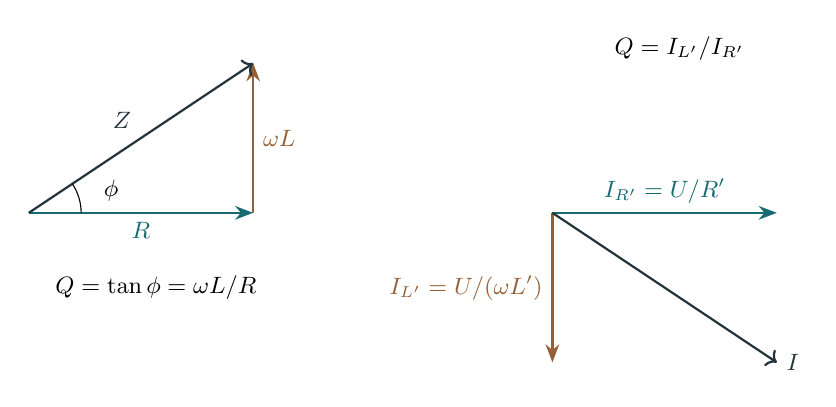
\begin{tikzpicture}[scale=.95,transform shape]

\begin{scope}
\draw[motion] (0,0)--(3,0) node[midway,below]{$R$};
\draw[force] (3,0)--(3,2) node[midway,right]{$\omega L$};
\draw[object,->] (0,0)--(3,2) node[midway,above left]{$Z$};
\draw (.7,0) arc(0:33.69:.7);\node at (1.1,.3){$\phi$};
\node at (1.7,-1){$Q=\tan\phi=\omega L/R$};
\end{scope}
\begin{scope}[shift={(7,0)}]
\draw[motion] (0,0)--(3,0) node[midway,above]{$I_{R'}=U/R'$};
\draw[force] (0,0)--(0,-2) node[midway,left]{$I_{L'}=U/(\omega L')$};
\draw[object,->] (0,0)--(3,-2) node[right]{$I$};
\node at (1.7,2.2){$Q=I_{L'}/I_{R'}$};
\end{scope}

\end{tikzpicture}
\figcaption{解图电5.9A\quad 阻抗的感性角与并联支路电流比描述同一品质因数}
\end{minipage}\end{center}

解图电5.9A中，串联模型同电流，$P_{\rm a}=I^2R$、$P_{\rm q}=I^2\omega L$，故$Q_s=\omega L/R$。并联模型同电压，$P_{\rm a}=U^2/R'$、$P_{\rm q}=U^2/(\omega L')$，故$Q_p=R'/(\omega L')$。代入转换式即得
\[
 \boxed{Q_s=Q_p=\frac{\omega L}{R}=\frac{R'}{\omega L'}.}
\]

解图电5.9B取变压器抽头为$D$，检测中点为$P$。将两个同相绕组电势明确规定为$\underline{\mathcal E}_1=V_A-V_D$、$\underline{\mathcal E}_2=V_D-V_B$，电流正向由A经$R_b$流向P，再由并联测量臂流向B。绕组电势在A到D到B的顺序上同向相加，这一极性约定决定了匝数比应放在哪一边。平衡时$V_P=V_D$、检流计无电流，电阻臂与待测并联臂承受的电势分别为$\underline{\mathcal E}_1,\underline{\mathcal E}_2$，两臂通过同一复电流$\underline I$：
\[
 \underline{\mathcal E}_1=R_b\underline I,\qquad
 \underline{\mathcal E}_2=Z_b\underline I,\qquad
 \frac{\underline{\mathcal E}_1}{\underline{\mathcal E}_2}=\frac{N_1}{N_2}.
\]
故$Y_b=1/Z_b=N_1/(N_2R_b)$为纯实数。对待测线圈采用并联模型，
\[
 Y_b=\frac1{R'}+j\left(\omega C-\frac1{\omega L'}\right).
\]
分别比较实部、虚部：
\[
 R'=\frac{N_2}{N_1}R_b,\qquad
 \omega C=\frac1{\omega L'}.
\]
于是
\[
 \boxed{Q=\frac{R'}{\omega L'}=\frac{N_2}{N_1}\omega C R_b.}
\]
检流计无电流要求相位也匹配，无功导纳必须恰好抵消，因此$R_b,C$提供两个可调条件。

\begin{center}\begin{minipage}{.98\linewidth}\centering
\begin{tikzpicture}[scale=.95,transform shape]
\begin{scope}[shift={(0.0,1.5)},rotate=90.0]\draw[object] (-1.5,0)--(-0.48,0) (0.48,0)--(1.5,0);\draw[object,fill=white] (-.48,-.14) rectangle (.48,.14);\end{scope}\node[anchor=east,fill=white,inner sep=1.5pt] at (-0.3400,1.5000) {$R_b$};
\draw[object] (0,3)--(4,3);
\begin{scope}[shift={(4.0,1.5)},rotate=-90.0]\draw[object] (-1.5,0)--(-0.48,0) (0.48,0)--(1.5,0);\draw[object,decorate,decoration={coil,aspect=.45,segment length=4pt,amplitude=3pt}] (-.48,0)--(.48,0);\end{scope}\node[anchor=west,fill=white,inner sep=1.5pt] at (4.3400,1.5000) {$L^\prime$};
\draw[object] (4,3)--(8,3);
\begin{scope}[shift={(6.0,1.5)},rotate=-90.0]\draw[object] (-1.5,0)--(-0.48,0) (0.48,0)--(1.5,0);\draw[object,fill=white] (-.48,-.14) rectangle (.48,.14);\end{scope}\node[anchor=west,fill=white,inner sep=1.5pt] at (6.3400,1.5000) {$R^\prime$};
\begin{scope}[shift={(8.0,1.5)},rotate=-90.0]\draw[object] (-1.5,0)--(-0.22,0) (0.22,0)--(1.5,0);\draw[object] (-.07,-.33)--(-.07,.33) (.07,-.33)--(.07,.33) (-.22,0)--(-.07,0) (.07,0)--(.22,0);\end{scope}\node[anchor=west,fill=white,inner sep=1.5pt] at (8.3400,1.5000) {$C$};
\draw[object] (8,0)--(4,0);
\begin{scope}[shift={(1.0,0.0)},rotate=0.0]\draw[object] (-1.0,0)--(-0.33,0) (0.33,0)--(1.0,0);\draw[object,fill=white] (0,0) circle (.33);\draw[object] plot[domain=-.23:.23,samples=35] (\x,{.12*sin(780*\x)});\end{scope}\node[anchor=north,fill=white,inner sep=1.5pt] at (1.0000,-0.3400) {$\mathcal E_1,\ N_1$};
\begin{scope}[shift={(3.0,0.0)},rotate=0.0]\draw[object] (-1.0,0)--(-0.33,0) (0.33,0)--(1.0,0);\draw[object,fill=white] (0,0) circle (.33);\draw[object] plot[domain=-.23:.23,samples=35] (\x,{.12*sin(780*\x)});\end{scope}\node[anchor=north,fill=white,inner sep=1.5pt] at (3.0000,-0.3400) {$\mathcal E_2,\ N_2$};\begin{scope}[shift={(2.0,1.5)},rotate=-90.0]\draw[object] (-1.5,0)--(-0.33,0) (0.33,0)--(1.5,0);\draw[object,fill=white] (0,0) circle (.33);\node[rotate=90.0] at (0,0) {$G$};\end{scope}
\fill (2,3) circle(.04) (2,0) circle(.04);
\node[above] at (2,3){$P$};\node[below] at (2,0){$D$};
\node[left] at (0,0){$A$};\node[right] at (4,0){$B$};
\draw[motion] (-1.1,.4)--(-1.1,2.3) node[midway,left]{$\underline I$};
\node at (3,-1.4){同相副绕组：$\mathcal E_1/\mathcal E_2=N_1/N_2$};
\node at (.45,.55){$+$};\node at (1.55,.55){$-$};
\node at (2.45,.55){$+$};\node at (3.55,.55){$-$};
\node[align=left,anchor=west]at(9.1,1.7){$\mathcal E_1=V_A-V_D$\\$\mathcal E_2=V_D-V_B$\\平衡时$V_P=V_D$\\检流计支流为零};

\end{tikzpicture}
\figcaption{解图电5.9B\quad 导纳电桥平衡：$P,D$等电势，待测线圈用并联模型}
\end{minipage}\end{center}


把两模型的同一端口功率也明确联系起来。以下$I,U$均为有效值，端口关系$U^2=I^2(R^2+\omega^2L^2)$。代入并联参数，
\[
\frac{U^2}{R'}=I^2R,\qquad
\frac{U^2}{\omega L'}=I^2\omega L.
\]
因此两模型不仅功率之比相同，而且同一激励下有功损耗和感性无功本身也分别相同。由反向换算直接相除，可把品质因数的代入过程写为
\[
\frac{\omega L}{R}
=\frac{\omega R'^2L'}{R'^2+(\omega L')^2}
\frac{R'^2+(\omega L')^2}{R'(\omega L')^2}
=\frac{R'}{\omega L'}.
\]
无功功率描述电感与外电路的周期储能交换；平均热耗散由电阻给出。只有$I^2R$或$U^2/R'$才是这只线圈平均转化为热的功率。

解图电5.9A使用一组具体的量值：$R=3\,\Omega$、$\omega L=2\,\Omega$。换算得$R'=13/3\,\Omega$、$\omega L'=13/2\,\Omega$。若端口电压有效值为13伏，并联两支流分别为3安和2安，故图A的阻抗三角形与电流三角形均给$Q=2/3$。这是图示所取的一个比例，一般线圈的Q仍由前面的公式确定。

桥的回路条件也应与等势条件一同写出。解图电5.9B中，检流计无流时$R_b$与整个并联测量臂通过同一个$\underline I$，因此
\[
\underline{\mathcal E}_1+\underline{\mathcal E}_2
=\underline I(R_b+Z_b),\qquad
\underline{\mathcal E}_1=\underline I R_b,\quad
\underline{\mathcal E}_2=\underline I Z_b.
\]
后两式还使用了$V_P=V_D$。它们相除才给$R_b/Z_b=N_1/N_2$，其中电阻臂和测量臂的压降分别对应 $N_1$ 和 $N_2$ 匝。整个测量臂导纳通分为
\[
Y_b=\frac1{R'}+\frac1{\mathrm j\omega L'}+\mathrm j\omega C
=\frac{\omega L'-\mathrm jR'(1-\omega^2L'C)}{R'\omega L'}.
\]
实部匹配给$1/R'=N_1/(N_2R_b)$，虚部零给$1-\omega^2L'C=0$；两个独立实条件要求两个可调量。电容电流抵消的是线圈的感性无功支流，并没有消除线圈电阻中的损耗。
\begin{center}\begin{minipage}{.97\linewidth}\centering
\begin{tikzpicture}[font=\small]
\draw[axis](-.4,0)--(4.6,0)node[right]{$\Re Y$};\draw[axis](0,-2.6)--(0,2.8)node[above]{$\Im Y$};
\draw[motion](0,0)--(3,0)node[above]{$G=1/R'$};
\draw[force](0,0)--(0,-2)node[left]{$B_L=-1/(\omega L')$};
\draw[blue,thick,-{Stealth}](0,0)--(0,2)node[left]{$B_C=\omega C$};
\draw[object,-{Stealth}](0,0)--(3,-2)node[below right]{$Y_{\text{线圈}}$};
\draw[guide](3,-2)--(3,0);
\node[align=left,anchor=west]at(5.5,.8){并联总导纳$Y_b=G+\mathrm j(B_L+B_C)$\\平衡：$B_C=-B_L$，$Y_b=G$\\线圈本身$Q=|B_L|/G$仍非零\\图取$R=3\,\Omega,\ \omega L=2\,\Omega$\\$G=3/13\,\mathrm S,\ |B_L|=2/13\,\mathrm S$\\横纵方向每单位长度均为$1/13\,\mathrm S$};
\end{tikzpicture}
\figcaption{解图电5.9C　电容与线圈的无功导纳反向抵消，留下正的电导。图中三条分量及线圈总导纳使用同一西门子标度。}
\end{minipage}\end{center}

解图电5.9C中，线圈导纳的虚部向下，电容导纳向上；$B_C+B_L=0$后，测量臂总导纳落到正实轴。线圈自身的电导G与感性导纳$B_L$都仍存在，故它自身的$Q=|B_L|/G=R'/(\omega L')$不为零。电桥让两条无功支流相消，再由共同电压下线圈的感性支流与损耗支流之比读出 $Q$。

平衡数据还能反求待测线圈的全部等效参数。记$k=N_2/N_1>0$，则
\[
R'=kR_b,\qquad L'=\frac1{\omega^2C},\qquad Q=k\omega CR_b,
\]
\[
R=\frac{kR_b}{1+Q^2},\qquad
L=\frac{Q^2}{1+Q^2}\frac1{\omega^2C}
=\frac{k^2R_b^2C}{1+Q^2}.
\]
这些式子同时保留电阻损耗、电感与测量频率；没有采用$Q\gg1$近似。把这两个串联参数代回 $\omega L/R$，即为由平衡读数得到的 $k\omega C R_b$。

两个调节量的作用还可由近于平衡的电势差看出。暂用高阻电压表检测P、D，使检测支流可忽略，取$\underline{\mathcal E}_2=E$为实参照，则$V_D=E,V_A=(1+1/k)E$。若测量臂导纳为$Y_b$，
\[
V_P-V_D=E\left[\frac{1+1/k}{1+R_bY_b}-1\right].
\]
在$Y_0=1/(kR_b)$附近、固定$R_b$，令$Y_b=Y_0+\delta Y$，一阶为
\[
V_P-V_D\simeq-\frac{kER_b}{k+1}\delta Y.
\]
电容微调给$\delta Y=\mathrm j\omega\delta C$，首先改变正交分量；实部比率误差则产生同相分量。这个局部式说明两旋钮为何分别调两个实条件。有限内阻的检流计接入时，可用这对节点的开路差压和等效阻抗计算表流。


\Needspace{13\baselineskip}

\pdfbookmark[2]{第 10 题 交流跳环的相位与平均斥力}{q10}

\section*{第 10 题\quad 交流跳环的相位与平均斥力}\label{q:10}


竖直铁棒上绕有接交流电源的线圈，棒上套一只铝环。接通开关时铝环跳起，适当调整电压可使其悬浮。解释该现象，证明平均磁力为斥力。铝环有电阻与自感，应作为$RL$串联回路；分析时采用线性磁响应、固定高度的局部周期稳态近似，并忽略铁损造成的额外相移。

\begin{center}\begin{minipage}{.98\linewidth}\centering
\begin{tikzpicture}[scale=.95,transform shape]

\draw[object,fill=rulegray] (-.4,-.5) rectangle (.4,4.7);
\foreach \y in {-.1,.35,.8,1.25,1.7,2.15}{\draw[object] (-1,\y) arc(180:360:1 and .3);}
\draw[object] (-1,2.15)--(-1,-.1) (1,2.15)--(1,-.1);
\draw[object,line width=1.2pt] (0,3.5) ellipse(1.5 and .4);
\node[right] at (1.7,3.5){铝环：$R,L$};
\draw[force] (0,3.8)--(0,5) node[above]{$\overline F_z$};
\node[right] at (1.3,1){交流线圈};
\draw[object] (-1,-.2)--(-2,-.2)--(-2,-1.4)--(2,-1.4)--(2,-.2)--(1,-.2);
\draw[object,fill=white] (0,-1.4) circle(.3);\node at (0,-1.4){$\sim$};
\node[left] at (-.5,4.5){铁棒};

\end{tikzpicture}
\figcaption{图电5.10\quad 端部非均匀交变磁场中的跳环}
\end{minipage}\end{center}

\Needspace{6\baselineskip}\subsection*{解答}


图电5.10中的励磁线圈电流设为$i_1=I_1\cos\omega t$。在线性近似下，穿环磁通与$i_1$同相，写作$\Phi_1=M I_1\cos\omega t$，其中$M>0$为该高度的互感。感应电动势
\[
 e_2=-\dot\Phi_1=\omega M I_1\sin\omega t
 =E_2\cos(\omega t-\pi/2).
\]
环有$R,L$，故其电流相对$e_2$再滞后
$\varphi=\arctan(\omega L/R)$：
\[
 i_2=I_2\cos(\omega t-\pi/2-\varphi),\qquad
 I_2=\frac{\omega M I_1}{\sqrt{R^2+\omega^2L^2}}.
\]
因此$i_2$相对$i_1$滞后$\delta=\pi/2+\varphi\in(\pi/2,\pi)$。在一个周期内，有些区间两电流同向，有些区间反向。

\begin{center}\begin{minipage}{.98\linewidth}\centering
\begin{tikzpicture}[scale=.95,transform shape]

\begin{scope}
\draw[object,fill=rulegray] (-.3,-.5) rectangle (.3,2.8);
\draw[object] (0,1.7) ellipse(1.5 and .35);
\draw[motion] (1.5,1.7)--(2.8,1.7) node[right]{$B_r$};
\draw[motion] (1.5,1.7)--(1.5,2.7) node[above]{$B_z$};
\node at (1.5,1.7){$\otimes$};\node[below right] at (1.6,1.3){$i_2$};
\draw[force] (1.5,1.7)--(1.5,.5) node[below]{$\dd F_z<0$};
\node at (.3,3.7){局部同向电流时吸引};
\end{scope}
\begin{scope}[shift={(7,0)}]
\draw[axis] (0,0)--(3.5,0) node[right]{$i_1,\Phi_1$};
\draw[axis] (0,0)--(0,-3) node[below]{$e_2$};
\draw[force] (0,0)--(-1.2,-2.078461) node[left]{$i_2$};
\draw[guide] (.7,0) arc(0:-90:.7);\node[right] at (.8,-.6){$\pi/2$};
\draw[guide](0,-1.1)arc(-90:-120:1.1);\node[left]at(-.65,-1.25){$\varphi=\pi/6$};
\node at (1.3,3){$\delta=2\pi/3=\pi/2+\varphi$};
\end{scope}

\end{tikzpicture}
\figcaption{解图电5.10A\quad 径向磁场给竖直力；感应与阻抗共同决定相位}
\end{minipage}\end{center}

解图电5.10A把磁场在环处的径向分量与轴向分量分开。左图按正励磁电流、正环流标出局部参考：环右端正电流流入纸面，径向场向右，其叉乘给向下的力。它用于定义吸引的符号；右图和图B取$\varphi=\pi/6$，在$t=0$实际环流为负，局部力因而向上；左图正电流的向下力在这一时刻反向。右图只用于比较相位，各量量纲不同，箭头长度不作幅值比例解释。径向分量同环电流作用产生竖直磁力；轴向分量主要产生环的径向胀缩力。取$z$向上，环离开线圈时耦合减弱，即$M'(z)<0$。在此局部模型中，竖直互作用力为
\[
 F_z=M'(z)i_1i_2.
\]
两个电流同向时吸引、$F_z<0$；反向时排斥、$F_z>0$。周期平均用
\[
 \langle\cos x\cos(x-\delta)\rangle=\tfrac12\cos\delta
 =-\tfrac12\sin\varphi,
\]
得到
\[
 \boxed{\overline F_z=-\frac12M'(z)I_1I_2\sin\varphi
 =-\frac{M'(z)M(z)\omega^2L I_1^2}
 {2(R^2+\omega^2L^2)}>0.}
\]
解图电5.10B的灰区内两电流同向，$M'<0$ 使这段产生向下的力。平均力取整个周期的有向面积：两电流乘积的平均为 $-I_1 I_2\sin\varphi/2$，再乘 $M'$ 得到向上的平均值。环有自感时，电流比励磁电流滞后超过四分之一周期。

\begin{center}\begin{minipage}{.98\linewidth}\centering
\begin{tikzpicture}[x=1.15cm,y=1.2cm,font=\small]
\fill[rulegray,opacity=.7]({pi/6},-1.17)rectangle({pi/2},1.17);
\fill[rulegray,opacity=.7]({7*pi/6},-1.17)rectangle({3*pi/2},1.17);
\draw[axis](0,0)--(6.95,0)node[right]{$\theta=\omega t$};
\draw[axis](0,-1.4)--(0,1.45)node[above]{归一化电流};
\foreach\v/\lab in{-1/-1,1/1}{\draw(0,\v)--(-.06,\v);\node[left]at(-.08,\v){$\lab$};}
\foreach\v in{1.570796,3.141593,4.712389,6.283185}{\draw(\v,0)--(\v,-.04);}
\node[below]at(3.141593,-.05){$\pi$};\node[below]at(6.283185,-.05){$2\pi$};
\draw[object,domain=0:6.283185,samples=150]plot(\x,{cos(deg(\x))});
\draw[traj,domain=0:6.283185,samples=150]plot(\x,{cos(deg(\x-2*pi/3))});
\node[align=left,anchor=west]at(7.9,.3){黑线：$i_1/I_1=\cos\theta$\\蓝线：$i_2/I_2=\cos(\theta-2\pi/3)$\\灰区：同向、向下吸引\\$\theta\in(\pi/6,\pi/2)$\\或$(7\pi/6,3\pi/2)$\\其余开区间反向、向上排斥};
\end{tikzpicture}
\figcaption{解图电5.10B\quad 有限自感使两电流反向的时间超过半个周期}
\end{minipage}\end{center}

若令$L\to0$而保留$R$，相差为$\pi/2$，吸引和排斥的平均抵消；若$R\to0$，相差趋向$\pi$，两者几乎总反向。实际铝环兼有电阻、自感，升高电压使$I_1$增大，平均力近似按$I_1^2$增大。当$\overline F_z=mg$可悬浮；若高度增加使平均力减小，则该竖直平衡具有恢复性。

刚接通时还会有暂态磁力。这里的周期平均用于解释持续悬浮。合闸阶段的环流由开关接通后的瞬时磁通和初始电流共同决定。


为把相位链与安培力计算逐步相接，先定义穿过环面的平均轴向磁场$B_\Phi(t)=B_{\Phi0}\cos\omega t$，环面积$S=\pi r^2$，于是$\Phi_1=SB_\Phi=MI_1\cos\omega t$、$E_2=\omega SB_{\Phi0}=\omega MI_1$。这里取的是穿环面的平均场；下面从圆周上的径向场计算竖直力。

固定高度下，令环边缘径向场$B_r(t)=B_{r0}\cos\omega t=b_rI_1\cos\omega t$，其中$b_r>0$。环流正向按图A右端流入纸面定义，竖直向上为正，故局部安培力$\dd F_z=-i_2B_r\dd l$，沿整个圆环积分为
\[
F_z(t)=-2\pi rB_{r0}I_2\cos\omega t\cos(\omega t-\delta)
=-K_F\cos\omega t\cos(\omega t-\delta),\qquad
K_F=2\pi rB_{r0}I_2>0.
\]
轴对称端部场的$B_r$沿环周处处径向向外，正环流与它叉乘处处向下，因此这些竖直分力相加，而不是相互抵消；轴向$B_z$与环流叉乘的径向分力则不能提供净竖直提升。

与互感方法之间也有明确对应。对半径固定的圆面，由磁通连续性$\nabla\!\cdot\!\mathbf B=0$及轴对称性，
\[
\frac{\partial\Phi_1}{\partial z}
=\int_S\frac{\partial B_z}{\partial z}\,\dd S
=-2\pi rB_r(r,z),\qquad
M'(z)i_1=-2\pi rB_r.
\]
所以$M'=-2\pi rb_r<0$，局部安培力式正好化为已有的$F_z=M'i_1i_2$，两种方法的力正向一致。这里环位置在一周期内近似不变，且场与励磁电流成线性关系。

将积化和差及周期积分完整写出，得到
\[
F_z(t)=-\frac{K_F}{2}[\cos\delta+\cos(2\omega t-\delta)],
\]
\[
\overline F_z=-\frac{K_F}{2T}
\int_0^T[\cos\delta+\cos(2\omega t-\delta)]\,\dd t
=-\frac{K_F}{2}\cos\delta
=\frac{K_F}{2}\sin\varphi>0.
\]
其中两倍频余弦在完整周期积分为零，留下相位差给出的常量。代入$K_F=-M'I_1I_2$和环电流幅值，就恢复框内的完整提升力公式。图B取$\delta=2\pi/3$，灰区两个同向区间总长度$2\pi/3$，占周期三分之一；其余三分之二反向排斥。一般相差$\delta\in(\pi/2,\pi)$时，反向比例为$\delta/\pi$，同向比例为$1-\delta/\pi$；上式的积分还计入两电流在各时刻的幅值乘积。
\begin{center}\begin{minipage}{.97\linewidth}\centering
\begin{tikzpicture}[x=.46cm,y=1.5cm,font=\small]
\begin{scope}[shift={(0,0)}]
\draw[axis](0,0)--(7.0,0)node[right]{$\theta$};\draw[axis](0,-.65)--(0,1.2);
\draw[guide](0,0)--(6.3,0);\node[right]at(4.3,.95){$\overline f=0$};
\draw[traj,domain=0:6.283185,samples=150]plot(\x,{-cos(deg(\x))*cos(deg(\x-pi/2))});
\node[above,align=center]at(3.1,1.45){电阻形式极限\\$\delta=\pi/2$};
\node[below]at(6.283185,-.08){$2\pi$};
\end{scope}
\begin{scope}[shift={(10,0)}]
\draw[axis](0,0)--(7.0,0)node[right]{$\theta$};\draw[axis](0,-.65)--(0,1.2);
\draw[guide](0,.25)--(6.3,.25);\node[right]at(6.35,.25){$\overline f=1/4$};
\draw[traj,domain=0:6.283185,samples=150]plot(\x,{-cos(deg(\x))*cos(deg(\x-2*pi/3))});
\node[above,align=center]at(3.1,1.45){实际RL示例\\$\delta=2\pi/3$};
\node[below]at(6.283185,-.08){$2\pi$};
\end{scope}
\begin{scope}[shift={(20,0)}]
\draw[axis](0,0)--(7.0,0)node[right]{$\theta$};\draw[axis](0,-.65)--(0,1.2);
\draw[guide](0,.5)--(6.3,.5);\node[right]at(6.35,.5){$\overline f=1/2$};
\draw[traj,domain=0:6.283185,samples=150]plot(\x,{-cos(deg(\x))*cos(deg(\x-pi))});
\node[above,align=center]at(3.1,1.45){无损周期分量\\$\delta=\pi$};
\node[below]at(6.283185,-.08){$2\pi$};
\end{scope}
\node[left]at(0,1.18){$f=F_z/K_F$};\end{tikzpicture}
\figcaption{解图电5.10C　三种相位关系的实际瞬时竖直力与平均线。向上为正，每面板各用自己的正幅度$K_F$归一化；无损面板只画无常量环流的周期分量。}
\end{minipage}\end{center}

解图电5.10C左图的电阻形式极限中$\delta=\pi/2$，力为$-(K_F/2)\sin2\omega t$，上下作用平均抵消。中图为图B同一相差，力为$K_F/4-(K_F/2)\cos(2\omega t-2\pi/3)$，瞬时仍有短时向下作用，平均却为$K_F/4$。右图$\delta=\pi$，周期分量给$F_z=K_F\cos^2\omega t\ge0$、平均$K_F/2$。图中比较的是归一化相位作用，改变R或L时$I_2$和$K_F$也会改变，实际力需要乘各自的 $K_F$。

若严格令R为零，环方程可积分为$Li_2+Mi_1=K$，常数K由初始磁链决定。已有周期分量为$-Mi_1/L$，还可叠加$K/L$的常量环流；它会改变瞬时力，而在固定高度、励磁电流均值为零时不改变平均互作用力。因此右图选择K为零，阻尼趋零的周期公式也可理解为$R\to0^+$的极限。这个初态限制与刚接通时另有暂态的说明相容。

悬浮高度由平均力与重力的交点给出。若只让M随高度变、R和L在局部近似固定，平均力与$-M(z)M'(z)$成正比；满足$\overline F_z(z_*)=mg$才是平衡，$\overline F_z'(z_*)<0$才有竖直恢复性。比如在适用范围内$M=M_0e^{-z/h}$，则$\overline F_z=Ae^{-2z/h}$，其中$A=M_0^2\omega^2LI_1^2/[2h(R^2+\omega^2L^2)]$。若存在该范围内的平衡，$z_*=(h/2)\ln[A/(mg)]$，线性小振动满足$\ddot\xi+(2g/h)\xi=0$；实际振动是否衰减还取决于阻尼。


\Needspace{13\baselineskip}

\pdfbookmark[2]{第 11 题 并联谐振的带宽、自由振荡与持久环流}{q11}

\section*{第 11 题\quad 并联谐振的带宽、自由振荡与持久环流}\label{q:11}


图中$L_1=10\,{\rm mH}$、$L_2=20\,{\rm mH}$、$C_1=10\,\mu{\rm F}$、$C_2=5\,\mu{\rm F}$、$R=100\,{\rm k}\Omega$。$L_1,C_1,C_2,L_2$依次跨接左右两母线，右母线在$C_1$下方标$A$、$C_2$上方标$B$。开关$K$长期闭合，将电阻与正弦恒流源接入母线；改变频率时电源电流振幅不变。
\begin{enumerate}
\item 有功功率最大值对应频率为$f_m$，半功率点为$f_-,f_+$，求$f_m/\Delta f$，其中$\Delta f=f_+-f_-$。
\item 打开$K$后，求四个储能元件的自由振荡频率。
\item 开关打开后某时刻$t_0$，两电感电流均以左向右为正，$i_{01}=0.1\,{\rm A},i_{02}=0.2\,{\rm A}$，母线左对右电压$U_0=40\,{\rm V}$。求$AB$内电流。
\item 求$L_1$中电流的振荡部分的振幅，说明给定瞬时数据意味着什么。
\end{enumerate}

\begin{center}\begin{minipage}{.98\linewidth}\centering
\begin{tikzpicture}[scale=.95,transform shape]
\begin{scope}[shift={(3.0,5.0)},rotate=0.0]\draw[object] (-3.0,0)--(-0.48,0) (0.48,0)--(3.0,0);\draw[object,decorate,decoration={coil,aspect=.45,segment length=4pt,amplitude=3pt}] (-.48,0)--(.48,0);\end{scope}\node[anchor=south,fill=white,inner sep=1.5pt] at (3.0000,5.3400) {$L_1$};
\begin{scope}[shift={(3.0,4.0)},rotate=0.0]\draw[object] (-3.0,0)--(-0.22,0) (0.22,0)--(3.0,0);\draw[object] (-.07,-.33)--(-.07,.33) (.07,-.33)--(.07,.33) (-.22,0)--(-.07,0) (.07,0)--(.22,0);\end{scope}\node[anchor=south,fill=white,inner sep=1.5pt] at (3.0000,4.3400) {$C_1$};
\begin{scope}[shift={(3.0,3.0)},rotate=0.0]\draw[object] (-3.0,0)--(-0.22,0) (0.22,0)--(3.0,0);\draw[object] (-.07,-.33)--(-.07,.33) (.07,-.33)--(.07,.33) (-.22,0)--(-.07,0) (.07,0)--(.22,0);\end{scope}\node[anchor=south,fill=white,inner sep=1.5pt] at (3.0000,3.3400) {$C_2$};
\begin{scope}[shift={(3.0,2.0)},rotate=0.0]\draw[object] (-3.0,0)--(-0.48,0) (0.48,0)--(3.0,0);\draw[object,decorate,decoration={coil,aspect=.45,segment length=4pt,amplitude=3pt}] (-.48,0)--(.48,0);\end{scope}\node[anchor=south,fill=white,inner sep=1.5pt] at (3.0000,2.3400) {$L_2$};
\begin{scope}[shift={(3.0,0.5)},rotate=0.0]\draw[object] (-3.0,0)--(-0.48,0) (0.48,0)--(3.0,0);\draw[object,fill=white] (-.48,-.14) rectangle (.48,.14);\end{scope}\node[anchor=south,fill=white,inner sep=1.5pt] at (3.0000,0.8400) {$R$};
\begin{scope}[shift={(3.0,-1.0)},rotate=0.0]\draw[object] (-3.0,0)--(-0.33,0) (0.33,0)--(3.0,0);\draw[object,fill=white] (0,0) circle (.33);\draw[motion] (-.21,0)--(.21,0);\end{scope}\node[anchor=south,fill=white,inner sep=1.5pt] at (3.0000,-0.6600) {$i_s(t)$};
\draw[object] (0,5)--(0,4);
\draw[object] (0,4)--(0,3);
\draw[object] (0,3)--(0,2);
\draw[object] (0,0.5)--(0,-1);
\draw[object] (6,5)--(6,4);
\draw[object] (6,4)--(6,3);
\draw[object] (6,3)--(6,2);
\draw[object] (6,0.5)--(6,-1);
\draw[object] (0,2)--(0,0.5);
\begin{scope}[shift={(6.0,1.25)},rotate=-90.0]\draw[object] (-0.75,0)--(-0.33,0) (0.33,0)--(0.75,0);\draw[object] (-.33,0)--(.27,.26);\fill (-.33,0) circle (.035) (.33,0) circle (.035);\end{scope}\node[anchor=west,fill=white,inner sep=1.5pt] at (6.3400,1.2500) {$K$};\node[right] at (6,3.8){$A$};\node[right] at (6,3.2){$B$};\node at (2.8,-1.8){频率可变、振幅恒定的电流源};
\end{tikzpicture}
\figcaption{图电5.11\quad 开关断开后上方四个储能元件仍闭合}
\end{minipage}\end{center}

\Needspace{6\baselineskip}\subsection*{解答}


先看图电5.11中闭合$K$的并联网络。等效参数为
\[
 C=C_1+C_2=15\,\mu{\rm F},\qquad
 L=\frac{L_1L_2}{L_1+L_2}=\frac{20}{3}\,{\rm mH}.
\]
总导纳及有功功率（$I$为电源电流有效值）为
\[
 Y=\frac1R+j\left(\Omega C-\frac1{\Omega L}\right),\quad
 P=\frac{I^2|Z|^2}{R}
 =\frac{I^2R}{1+R^2(\Omega C-1/(\Omega L))^2}.
\]
恒流驱动下，阻抗最大时电压、功率最大，故
\[
 \Omega_m=\frac1{\sqrt{LC}},\qquad P_{\max}=I^2R.
\]
半功率条件是$\Omega_\pm C-1/(\Omega_\pm L)=\pm1/R$，解二次式：
\[
 \Omega_\pm=\frac{\sqrt{R^{-2}+4C/L}\ \pm R^{-1}}{2C}.
\]
两根相减得$\Delta\Omega=1/(RC)$，所以
\[
 \boxed{\frac{f_m}{\Delta f}=R\sqrt{\frac CL}
 =4743.4165.}
\]
代入 $C=15\times10^{-6}\,\mathrm F$、$L=(20/3)\times10^{-3}\,\mathrm H$，求得峰频 $f_m=503.2921\,{\rm Hz}$、带宽 $\Delta f=0.1061033\,{\rm Hz}$。前者用 $1/(2\pi\sqrt{LC})$，后者用 $1/(2\pi RC)$。

\begin{center}\begin{minipage}{.98\linewidth}\centering
\begin{tikzpicture}[x=1.2cm,y=3cm,font=\small]
\draw[axis](-3.25,0)--(3.45,0)node[right]{$x$};\draw[axis](-3.15,0)--(-3.15,1.18)node[above]{$P/P_{\max}$};
\draw[guide](-3.15,.5)--(3.1,.5);\node[left]at(-3.15,.5){$1/2$};\node[left]at(-3.15,1){$1$};
\draw[traj,domain=-3:3,samples=155]plot(\x,{1/(1+((2*\x+\x*\x/4743.416490253)/(1+\x/4743.416490253))^2)});
\draw[guide](-.499973648,0)--(-.499973648,.5)(.500026352,0)--(.500026352,.5)(0,0)--(0,1);
\node[below]at(-.65,-.015){$x_-$};\node[below]at(.65,-.015){$x_+$};\node[above right]at(0,1){$f_m$};
\draw[force,<->](-.499973648,.15)--(.500026352,.15);
\node[align=left,anchor=west]at(4.3,.72){$x=(f-f_m)/\Delta f$\\$f_m=503.292121\,\mathrm{Hz}$\\$\Delta f=0.1061033\,\mathrm{Hz}$\\$x_-=-0.499973648$\\$x_+=0.500026352$\\两根的精确间距为1};
\end{tikzpicture}
\figcaption{解图电5.11A\quad 以实际峰频和带宽为尺度的精确功率曲线；两个半功率点由完整方程计算}
\end{minipage}\end{center}

解图电5.11A使用$x=(f-f_m)/\Delta f$，纵轴是实际$P/P_{\max}$，曲线代入本题精确导纳式；两个半功率点分别由曲线求得。其稳定的作图表达式为
\[
\frac P{P_{\max}}=\frac1{1+[(2x+x^2/Q_b)/(1+x/Q_b)]^2},\qquad
Q_b=\frac{f_m}{\Delta f}=4743.416490253.
\]
因为$Q_b$很大，两个半功率横坐标看上去接近$\pm1/2$，实际为$-0.499973648$和$0.500026352$。绝对频率分别为$f_-=503.239072193\,\mathrm{Hz}$、$f_+=503.345175489\,\mathrm{Hz}$，相减恢复给出的带宽。打开$K$后，电阻与电源退出，剩下无损并联$LC$，故自由振荡频率仍为
\[
 \boxed{f_0=\frac1{2\pi\sqrt{LC}}=503.2921\,{\rm Hz}.}
\]
并且$L_1C_1=L_2C_2=10^{-7}\,{\rm s^2}$，两组的固有频率恰相同。

再看解图电5.11B。设电感电流均从左向右，电容电流也以左向右为正。共用电压$u$使$i_{C1}/i_{C2}=C_1/C_2=2$，无外接电流时
\[
 i_{C1}+i_{C2}=-(i_{01}+i_{02})=-0.3\,{\rm A}.
\]
因此$i_{C1}=-0.2\,{\rm A}$、$i_{C2}=-0.1\,{\rm A}$。在$A$节点，流向$B$的电流为
\[
 \boxed{i_{AB}=i_{01}+i_{C1}=-0.1\,{\rm A},}
\]
即实际$0.1\,{\rm A}$由$B$流向$A$。

\begin{center}\begin{minipage}{.98\linewidth}\centering
\begin{tikzpicture}[scale=.95,transform shape]
\begin{scope}[shift={(2.5,4.0)},rotate=0.0]\draw[object] (-2.5,0)--(-0.48,0) (0.48,0)--(2.5,0);\draw[object,decorate,decoration={coil,aspect=.45,segment length=4pt,amplitude=3pt}] (-.48,0)--(.48,0);\end{scope}\node[anchor=south,fill=white,inner sep=1.5pt] at (2.5000,4.3400) {$L_1$};
\begin{scope}[shift={(2.5,3.0)},rotate=0.0]\draw[object] (-2.5,0)--(-0.22,0) (0.22,0)--(2.5,0);\draw[object] (-.07,-.33)--(-.07,.33) (.07,-.33)--(.07,.33) (-.22,0)--(-.07,0) (.07,0)--(.22,0);\end{scope}\node[anchor=south,fill=white,inner sep=1.5pt] at (2.5000,3.3400) {$C_1$};
\begin{scope}[shift={(2.5,1.0)},rotate=0.0]\draw[object] (-2.5,0)--(-0.22,0) (0.22,0)--(2.5,0);\draw[object] (-.07,-.33)--(-.07,.33) (.07,-.33)--(.07,.33) (-.22,0)--(-.07,0) (.07,0)--(.22,0);\end{scope}\node[anchor=south,fill=white,inner sep=1.5pt] at (2.5000,1.3400) {$C_2$};
\begin{scope}[shift={(2.5,0.0)},rotate=0.0]\draw[object] (-2.5,0)--(-0.48,0) (0.48,0)--(2.5,0);\draw[object,decorate,decoration={coil,aspect=.45,segment length=4pt,amplitude=3pt}] (-.48,0)--(.48,0);\end{scope}\node[anchor=south,fill=white,inner sep=1.5pt] at (2.5000,0.3400) {$L_2$};
\draw[object] (0,4)--(0,3);
\draw[object] (0,3)--(0,1);
\draw[object] (0,1)--(0,0);
\draw[object] (5,4)--(5,3);
\draw[object] (5,3)--(5,1);
\draw[object] (5,1)--(5,0);
\draw[motion] (3.5,4.25)--(4.6,4.25) node[midway,above]{$i_1=0.1$};
\draw[motion] (3.5,-.4)--(4.6,-.4) node[midway,below]{$i_2=0.2$};
\draw[motion] (3.5,3.3)--(4.6,3.3) node[midway,above]{$i_{C1}=-0.2$};
\draw[motion] (3.5,.6)--(4.6,.6) node[midway,below]{$i_{C2}=-0.1$};
\draw[force] (5.4,2.7)--(5.4,1.3) node[midway,right]{$i_{AB}=-0.1\,{\rm A}$};
\node[above right] at (5,2.7){$A$};\node[below right] at (5,1.3){$B$};
\node at (2.5,-1.3){电流数字单位均为${\rm A}$；负值表示反向};

\end{tikzpicture}
\figcaption{解图电5.11B\quad 瞬时节点守恒与桥段的持久环流}
\end{minipage}\end{center}

桥段电流在整个自由响应中保持这个值。由$L_1\dot i_1=L_2\dot i_2=u$，
$L_1i_1-L_2i_2$为常量；又因$L_1C_1=L_2C_2$，
\[
 i_{AB}=\frac{C_2i_1-C_1i_2}{C_1+C_2}
 =\frac{i_1-2i_2}{3}=-0.1\,{\rm A}.
\]
于是$L_1$电流包含持久环流$i_{\rm d}=-0.1\,{\rm A}$和振荡部分$i_{1r}$。在$t_0$，
$i_{1r}=i_{01}-i_{\rm d}=0.2\,{\rm A}$。独立振荡能量给
\[
 \frac12L_1 I_{1r}^2
 =\frac12L_1(0.2)^2+\frac12C_1(40)^2,
\]
故
\[
 \boxed{I_{1r}=\sqrt{0.2^2+\frac{C_1}{L_1}40^2}
 =1.280625\,{\rm A}.}
\]
以$t_0$为新原点，完整电流还可写成
\[
 i_1(t)=-0.1+0.2\cos\omega_0t+
 \frac{40}{L_1\omega_0}\sin\omega_0t\quad({\rm A}).
\]
振荡幅度从负0.1安的中心量起，完整电流的最大绝对值从零量起。给定数据$i_1\ne2i_2$表明有非振荡环流；它可由先前初态保留在两只理想电感构成的闭环中，不必据此断言电源含直流。若另规定从全零初态仅由纯正弦源建立响应，则该环流不产生，此组瞬时数据与那项附加规定不相容。


展开半功率条件，可同时求两根的差和积。恒流驱动时只有电阻消耗平均有功，$P=U^2/R$，因此把完整导纳模代入后得到的半功率条件为
\[
R^{-2}=(\Omega C-1/(\Omega L))^2.
\]
分别取正、负支，乘以正的$\Omega L$，得到两个二次方程
\[
LC\Omega_+^2-(L/R)\Omega_+-1=0,\qquad
LC\Omega_-^2+(L/R)\Omega_--1=0.
\]
各取正根即为前面的$\Omega_\pm$。相减给严格带宽，不需窄带近似；两根相乘另有$\Omega_+\Omega_-=1/(LC)=\Omega_m^2$，所以峰频是两个半功率频率的几何平均；算术平均略高于峰频。题设$C=1.5\times10^{-5}\,\mathrm F$、$L=(20/3)\times10^{-3}\,\mathrm H$，两者乘积$10^{-7}\,\mathrm{s^2}$，独立决定$\Omega_m=3162.277660\,\mathrm{s^{-1}}$。

内部电流由解图电5.11B的四条支路求出。开关打开后，对右母线全部四支路，
\[
i_1+i_2+(C_1+C_2)\dot u=0,\qquad
L_1\dot i_1=L_2\dot i_2=u.
\]
定义总电感电流$I_\Sigma=i_1+i_2$与磁链差$\mathcal K=L_1i_1-L_2i_2$，立刻有
\[
\dot I_\Sigma=\frac uL,\qquad C\dot u=-I_\Sigma,\qquad
\dot{\mathcal K}=0.
\]
因此自由响应包含一个频率$\omega_0=1/\sqrt{LC}$的振荡模式和一个零频环流模式。两组$L_1C_1$、$L_2C_2$相等保证相容的振荡部分有相同频率；共用电压把两组振荡的相位联系起来。

从总电流和磁链差反解，得到完整分解：
\[
i_{\mathrm d}=\frac{\mathcal K}{L_1+L_2},\qquad
i_1=\frac{L_2}{L_1+L_2}I_\Sigma+i_{\mathrm d},\qquad
i_2=\frac{L_1}{L_1+L_2}I_\Sigma-i_{\mathrm d}.
\]
本题$\mathcal K=(0.01)(0.1)-(0.02)(0.2)=-0.003\,\mathrm{Wb}$，故$i_{\mathrm d}=-0.1\,\mathrm A$。两只电感的恒定部分方向相反，端口总电流为零；给定时刻的振荡部分则为$i_{1r}=0.2\,\mathrm A$、$i_{2r}=0.1\,\mathrm A$。图B中桥段的恒流正是$i_{\mathrm d}$，其负号说明实际从B流向A。

以$t_0$为新原点，用$u(0)=40\,\mathrm V,I_\Sigma(0)=0.3\,\mathrm A$解两个一阶方程，
\[
\begin{aligned}
I_\Sigma(t)&=0.3\cos\omega_0t+\frac{40}{L\omega_0}\sin\omega_0t,\\
u(t)&=40\cos\omega_0t-\frac{0.3}{C\omega_0}\sin\omega_0t,\\
i_2(t)&=0.1+0.1\cos\omega_0t+\frac{40}{L_2\omega_0}\sin\omega_0t.
\end{aligned}
\]
与前面完整$i_1(t)$相加、相减，分别恢复总电流和恒定磁链差。再求导，可在任意时刻验证$\dot i_1=u/L_1$、$\dot i_2=u/L_2$和两电容电流比，因此桥段恒流并不是只在给定时刻偶然成立。

振幅的能量计算也应先作同样分解。完整储能严格分成
\[
H=\frac12L_1i_1^2+\frac12L_2i_2^2+\frac12Cu^2
=\underbrace{\frac12LI_\Sigma^2+\frac12Cu^2}_{H_{\mathrm{osc}}}
+\underbrace{\frac{\mathcal K^2}{2(L_1+L_2)}}_{H_{\mathrm d}}.
\]
本题$H_{\mathrm{osc}}=0.0123\,\mathrm J$、$H_{\mathrm d}=0.00015\,\mathrm J$，总能量$0.01245\,\mathrm J$。恒流部分储能不会转化成所求的振荡振幅。由于$L_1C_1=L_2C_2$，还可将振荡能量分别写成
\[
H_{1r}=\frac12L_1i_{1r}^2+\frac12C_1u^2=0.0082\,\mathrm J,\qquad
H_{2r}=\frac12L_2i_{2r}^2+\frac12C_2u^2=0.0041\,\mathrm J.
\]
它们之和等于$H_{\mathrm{osc}}$。第一式正是前面求$1.280625$安的能量依据；若把总电感电流0.1安代入，就将偏置和振荡量混在一起。电压幅值为$U_a=\sqrt{40^2+[0.3/(C\omega_0)]^2}=40.496913\,\mathrm V$。
\begin{center}\begin{minipage}{.97\linewidth}\centering
\begin{tikzpicture}[scale=.85,transform shape,font=\small]
\draw[axis](-2.5,0)--(2.7,0)node[right]{$x$};\draw[axis](0,-2.5)--(0,2.7)node[above]{$y$};
\draw[object](0,0)circle(2);
\draw[traj,-{Stealth}](.684040,1.879385)arc(70:45:2);
\fill[accent](.312348,1.975459)circle(.055);\node[above right,fill=white,inner sep=1pt]at(.312348,1.975459){$P_0$};
\node[align=left,anchor=west]at(3.65,.8){$x=(i_1-i_{\mathrm d})/(1.280625\,\mathrm A)$\\$y=u/(40.496913\,\mathrm V)$\\$i_{\mathrm d}=-0.1\,\mathrm A$\\$P_0:\ x=0.156174,\ y=0.987730$\\$x^2+y^2=1$，沿顺时针运动\\本图已扣去恒定环流};
\end{tikzpicture}
\figcaption{解图电5.11C　扣除恒定环流后的归一化相平面。圆周表示同一振荡能量，给定状态$P_0$位于第一象限，电感电流增加、电容电压下降。}
\end{minipage}\end{center}

解图电5.11C用不同物理单位分别归一化，$x^2+y^2=1$与$H_{1r}$守恒等价。由$\dot i_{1r}=u/L_1$、$\dot u=-i_{1r}/C_1$，归一化方程为$\dot x=\omega_0y,\dot y=-\omega_0x$，轨迹沿顺时针；在$P_0$处$x,y$均正，电流向其正峰值推进。若不扣除$i_{\mathrm d}$，在未经归一化的$(i_1,u)$平面中能量曲线中心应为$i_1=-0.1$安。

最后明确给定初态的含义：即使开关K仍闭合、有电阻和电源接入，两只理想并联电感也始终承受同一端口电压，故$\dot{\mathcal K}=0$对任意端口波形都成立。全零初态的$\mathcal K=0$不能被共同驱动变成这里的$-0.003$韦伯；即使电源另外含直流也不改变这条守恒。长期闭合的并联电阻只能耗散可见于端口的暂态，不能自动消除两电感零端电压的反向环流。因此这些瞬时数据规定了独立的预存环流初态，需要与接通前的准备状态相容；共同端口的交流与直流都保持同一个磁链差。


\Needspace{13\baselineskip}

\pdfbookmark[2]{第 12 题 无限电感电容链的色散与传播速度}{q12}

\section*{第 12 题\quad 无限电感电容链的色散与传播速度}\label{q:12}


无限网络由串联电感$L$及每个节点对公共回线接的电容$C$构成，单节长度为$l$。角频率为$\omega$的正弦波向右传播，相邻电容电压的相位滞后为$\varphi$。
\begin{enumerate}
\item 求$\varphi(\omega,L,C)$并给出传播频段。
\item 求波的相位传播速度。
\item 在什么条件下速度几乎与$\omega$无关？求该极限速度，并区分相速度与波包群速度。
\end{enumerate}

\begin{center}\begin{minipage}{.98\linewidth}\centering
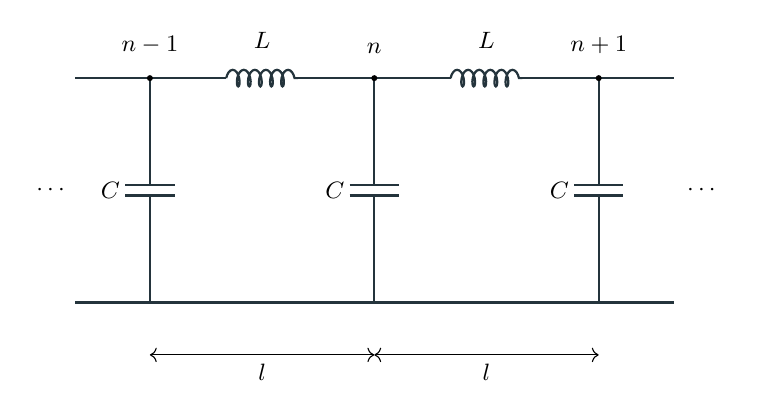
\begin{tikzpicture}[scale=.95,transform shape]
\begin{scope}[shift={(0.0,1.5)},rotate=-90.0]\draw[object] (-1.5,0)--(-0.22,0) (0.22,0)--(1.5,0);\draw[object] (-.07,-.33)--(-.07,.33) (.07,-.33)--(.07,.33) (-.22,0)--(-.07,0) (.07,0)--(.22,0);\end{scope}\node[anchor=east,fill=white,inner sep=1.5pt] at (-0.3400,1.5000) {$C$};
\begin{scope}[shift={(3.0,1.5)},rotate=-90.0]\draw[object] (-1.5,0)--(-0.22,0) (0.22,0)--(1.5,0);\draw[object] (-.07,-.33)--(-.07,.33) (.07,-.33)--(.07,.33) (-.22,0)--(-.07,0) (.07,0)--(.22,0);\end{scope}\node[anchor=east,fill=white,inner sep=1.5pt] at (2.6600,1.5000) {$C$};
\begin{scope}[shift={(6.0,1.5)},rotate=-90.0]\draw[object] (-1.5,0)--(-0.22,0) (0.22,0)--(1.5,0);\draw[object] (-.07,-.33)--(-.07,.33) (.07,-.33)--(.07,.33) (-.22,0)--(-.07,0) (.07,0)--(.22,0);\end{scope}\node[anchor=east,fill=white,inner sep=1.5pt] at (5.6600,1.5000) {$C$};
\begin{scope}[shift={(1.5,3.0)},rotate=0.0]\draw[object] (-1.5,0)--(-0.48,0) (0.48,0)--(1.5,0);\draw[object,decorate,decoration={coil,aspect=.45,segment length=4pt,amplitude=3pt}] (-.48,0)--(.48,0);\end{scope}\node[anchor=south,fill=white,inner sep=1.5pt] at (1.5000,3.3400) {$L$};
\begin{scope}[shift={(4.5,3.0)},rotate=0.0]\draw[object] (-1.5,0)--(-0.48,0) (0.48,0)--(1.5,0);\draw[object,decorate,decoration={coil,aspect=.45,segment length=4pt,amplitude=3pt}] (-.48,0)--(.48,0);\end{scope}\node[anchor=south,fill=white,inner sep=1.5pt] at (4.5000,3.3400) {$L$};
\draw[object] (0,0)--(3,0);
\draw[object] (3,0)--(6,0);\draw[object] (-1,3)--(0,3) (6,3)--(7,3) (-1,0)--(0,0) (6,0)--(7,0);\node at (-1.3,1.5){$\cdots$};\node at (7.4,1.5){$\cdots$};\fill (0,3) circle(.04);\node[above] at (0,3.2) {$n-1$};\fill (3,3) circle(.04);\node[above] at (3,3.2) {$n$};\fill (6,3) circle(.04);\node[above] at (6,3.2) {$n+1$};\draw[<->] (0,-.7)--(3,-.7) node[midway,below]{$l$};\draw[<->] (3,-.7)--(6,-.7) node[midway,below]{$l$};
\end{tikzpicture}
\figcaption{图电5.12\quad 一节一个串联电感和一个并联电容}
\end{minipage}\end{center}

\Needspace{6\baselineskip}\subsection*{解答}


图电5.12的节点编号由左向右增加，令$u_n$为节点对回线电压，$i_n$为从$n$到$n+1$流过电感的电流。解图电5.12A中两个基本关系为
\[
 L\dot i_n=u_n-u_{n+1},\qquad
 C\dot u_n=i_{n-1}-i_n.
\]
第二式求导并代第一式，得到离散波动方程
\[
 LC\ddot u_n=u_{n-1}-2u_n+u_{n+1}.
\]

\begin{center}\begin{minipage}{.98\linewidth}\centering
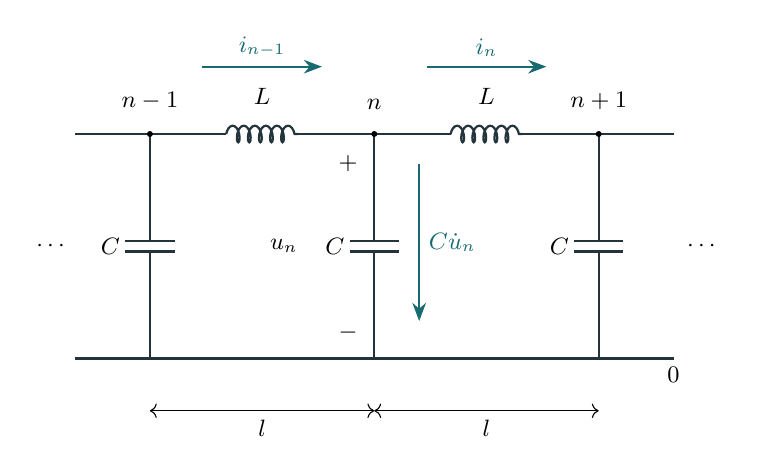
\begin{tikzpicture}[scale=.95,transform shape]
\begin{scope}[shift={(0.0,1.5)},rotate=-90.0]\draw[object] (-1.5,0)--(-0.22,0) (0.22,0)--(1.5,0);\draw[object] (-.07,-.33)--(-.07,.33) (.07,-.33)--(.07,.33) (-.22,0)--(-.07,0) (.07,0)--(.22,0);\end{scope}\node[anchor=east,fill=white,inner sep=1.5pt] at (-0.3400,1.5000) {$C$};
\begin{scope}[shift={(3.0,1.5)},rotate=-90.0]\draw[object] (-1.5,0)--(-0.22,0) (0.22,0)--(1.5,0);\draw[object] (-.07,-.33)--(-.07,.33) (.07,-.33)--(.07,.33) (-.22,0)--(-.07,0) (.07,0)--(.22,0);\end{scope}\node[anchor=east,fill=white,inner sep=1.5pt] at (2.6600,1.5000) {$C$};
\begin{scope}[shift={(6.0,1.5)},rotate=-90.0]\draw[object] (-1.5,0)--(-0.22,0) (0.22,0)--(1.5,0);\draw[object] (-.07,-.33)--(-.07,.33) (.07,-.33)--(.07,.33) (-.22,0)--(-.07,0) (.07,0)--(.22,0);\end{scope}\node[anchor=east,fill=white,inner sep=1.5pt] at (5.6600,1.5000) {$C$};
\begin{scope}[shift={(1.5,3.0)},rotate=0.0]\draw[object] (-1.5,0)--(-0.48,0) (0.48,0)--(1.5,0);\draw[object,decorate,decoration={coil,aspect=.45,segment length=4pt,amplitude=3pt}] (-.48,0)--(.48,0);\end{scope}\node[anchor=south,fill=white,inner sep=1.5pt] at (1.5000,3.3400) {$L$};
\begin{scope}[shift={(4.5,3.0)},rotate=0.0]\draw[object] (-1.5,0)--(-0.48,0) (0.48,0)--(1.5,0);\draw[object,decorate,decoration={coil,aspect=.45,segment length=4pt,amplitude=3pt}] (-.48,0)--(.48,0);\end{scope}\node[anchor=south,fill=white,inner sep=1.5pt] at (4.5000,3.3400) {$L$};
\draw[object] (0,0)--(3,0);
\draw[object] (3,0)--(6,0);\draw[object] (-1,3)--(0,3) (6,3)--(7,3) (-1,0)--(0,0) (6,0)--(7,0);\node at (-1.3,1.5){$\cdots$};\node at (7.4,1.5){$\cdots$};\fill (0,3) circle(.04);\node[above] at (0,3.2) {$n-1$};\fill (3,3) circle(.04);\node[above] at (3,3.2) {$n$};\fill (6,3) circle(.04);\node[above] at (6,3.2) {$n+1$};\draw[<->] (0,-.7)--(3,-.7) node[midway,below]{$l$};\draw[<->] (3,-.7)--(6,-.7) node[midway,below]{$l$};\draw[motion] (.7,3.9)--(2.3,3.9) node[midway,above]{$i_{n-1}$};\draw[motion] (3.7,3.9)--(5.3,3.9) node[midway,above]{$i_n$};\draw[motion] (3.6,2.6)--(3.6,.5) node[midway,right]{$C\dot u_n$};\node[left] at (2.1,1.5){$u_n$};\node[below]at(7,0){$0$};\node at(2.65,2.6){$+$};\node at(2.65,.35){$-$};
\end{tikzpicture}
\figcaption{解图电5.12A\quad 相邻电感电流之差给节点电容电流}
\end{minipage}\end{center}

对向右行进、等幅的波，写
$u_n=U_0\cos(\omega t-n\varphi)$，故
$u_{n-1}+u_{n+1}=2u_n\cos\varphi$。代入得
\[
 \boxed{\omega^2LC=2(1-\cos\varphi)=4\sin^2\frac\varphi2.}
\]
取第一传播支$0\le\varphi\le\pi$，
\[
 \boxed{\varphi=2\arcsin\frac{\omega\sqrt{LC}}2
 =\arccos\left(1-\frac{\omega^2LC}{2}\right).}
\]
需有实相位，传播带为$0\le\omega\le2/\sqrt{LC}$。超过上截止频率时，不再有这种等幅行波，而是空间衰减的响应；端点$\varphi=\pi$处相邻节点反相，群速度为零。

相同相位从$n$移至$n+1$需$\Delta t=\varphi/\omega$，故相速度为
\[
 \boxed{v_p=\frac{\omega l}{\varphi}
 =\frac{\omega l}{2\arcsin(\omega\sqrt{LC}/2)}.}
\]
解图电5.12B横轴为$\varphi=kl$，纵轴为$\omega\sqrt{LC}$，均已无量纲化。过原点的割线斜率是$v_p/v_0$，在P点的切线斜率是$v_g/v_0$，其中$v_0=l/\sqrt{LC}$；实际速度须乘回这一尺度。波包群速度由未归一化的$\omega(k)$求导：
\[
 \omega(k)=\frac2{\sqrt{LC}}\sin\frac{kl}{2},\qquad
 \boxed{v_g=\frac{\dd\omega}{\dd k}=\frac l{\sqrt{LC}}\cos\frac\varphi2.}
\]
一般$v_g\ne v_p$；相速度跟随固定相位，群速度跟随窄带波包的包络。

\begin{center}\begin{minipage}{.98\linewidth}\centering
\begin{tikzpicture}[x=2cm,y=2cm,font=\small]
\draw[axis](0,0)--(3.55,0)node[right]{$\varphi=kl$};\draw[axis](0,0)--(0,2.32)node[above]{$\omega\sqrt{LC}$};
\draw[traj,domain=0:3.141593,samples=130]plot(\x,{2*sin(deg(\x/2))});
\draw[motion](0,0)--({pi/3},1);
\draw[force](.2,{1+sqrt(3)/2*(.2-pi/3)})--(2.3,{1+sqrt(3)/2*(2.3-pi/3)});
\fill[accent]({pi/3},1)circle(.025);\node[above left]at({pi/3},1){$P$};
\draw[guide]({pi/3},0)--({pi/3},1)--(0,1)(0,2)--({pi},2)--({pi},0);
\node[below]at({pi/3},0){$\pi/3$};\node[below]at(pi,0){$\pi$};\node[left]at(0,1){$1$};\node[left]at(0,2){$2$};
\node[align=left,anchor=west]at(4.1,1.45){$v_0=l/\sqrt{LC}$\\横纵轴均为无量纲量\\割线斜率$=v_p/v_0$\\切线斜率$=v_g/v_0$\\图取$P:(\pi/3,1)$\\$v_p/v_0=3/\pi$\\$v_g/v_0=\sqrt3/2$};
\end{tikzpicture}
\figcaption{解图电5.12B\quad 归一化色散曲线的割线与切线给相速度比和群速度比}
\end{minipage}\end{center}

当$\omega\sqrt{LC}\ll1$（等价于$\varphi\ll1$、波长远大于$l$），
\[
 \varphi=\omega\sqrt{LC}+\frac{(\omega\sqrt{LC})^3}{24}+\cdots,
\]
\[
 v_p=\frac l{\sqrt{LC}}\left[1-\frac{\omega^2LC}{24}+\cdots\right],
 \quad
 v_g=\frac l{\sqrt{LC}}\left[1-\frac{\omega^2LC}{8}+\cdots\right].
\]
两者都近似为$\boxed{v_0=l/\sqrt{LC}}$，此时才可把网络近似成无色散的连续传输线。


为求相邻节点间电感电流的半节相位，先写各支路的周期电流。取$\theta_n=\omega t-n\varphi$，节点电压按余弦变化。电容支流以向下为正，得到
\[
i_{C,n}=C\dot u_n=-\omega CU_0\sin\theta_n.
\]
相邻节点电压差按图A中电感电流的正向，从左到右取压降。由余弦差公式，
\[
u_n-u_{n+1}=U_0[\cos\theta_n-\cos(\theta_n-\varphi)]
=-2U_0\sin\frac\varphi2\sin\left(\theta_n-\frac\varphi2\right).
\]
电感关系$L\dot i_n=u_n-u_{n+1}$给单频周期电流
\[
i_n=\frac{2U_0}{\omega L}\sin\frac\varphi2
\cos\left(\theta_n-\frac\varphi2\right),\qquad
i_{n-1}=\frac{2U_0}{\omega L}\sin\frac\varphi2
\cos\left(\theta_n+\frac\varphi2\right).
\]
这一步是在选定的单频行波中积分，不另加独立直流支流；若采用正弦电压参照，所有时间相位共同平移四分之一周期，结论相同。两电感电流在节点相减后
\[
i_{n-1}-i_n=-\frac{4U_0}{\omega L}\sin^2\frac\varphi2\sin\theta_n.
\]
与$i_{C,n}$比较同一谐波的幅系数，重新得到$\omega^2LC=4\sin^2(\varphi/2)$。它是对任意时刻成立的函数恒等式；比较的是正弦项的系数。电感电流的相位居于两端节点电压相位的中间，差半节。
\begin{center}\begin{minipage}{.97\linewidth}\centering
\begin{tikzpicture}[font=\small]
\begin{scope}
\draw[axis](-.2,0)--(2.8,0);\draw[axis](0,-2)--(0,2);
\draw[motion](0,0)--(2,0)node[above]{$U_n$};
\draw[traj,-{Stealth}](0,0)--(1,-1.732051)node[below]{$U_{n+1}$};
\draw[force](1,-1.732051)--(2,0)node[midway,right]{$U_{L,n}$};
\node[above]at(1,2.3){电压以$U_0$为单位};
\node[below,align=center]at(1.3,-2.35){$U_{L,n}=U_n-U_{n+1}$\\差矢量由$U_{n+1}$端点指向$U_n$端点};
\end{scope}
\begin{scope}[shift={(6.8,0)}]
\draw[axis](-.2,0)--(2.8,0);\draw[axis](0,-1.8)--(0,2.2);
\draw[motion](0,0)--(1.732051,-1)node[below right]{$I_n$};
\draw[traj,-{Stealth}](0,0)--(1.732051,1)node[above right]{$I_{n-1}$};
\draw[force](1.732051,-1)--(1.732051,1)node[midway,right]{$I_{C,n}$};
\draw[guide](0,2)--(1.732051,1);
\node[above]at(1.1,2.3){电流以$U_0/(\omega L)$为单位};
\node[below,align=center]at(1.3,-2.35){$I_{C,n}=I_{n-1}-I_n$\\各面板横纵等标度，坐标均放大2倍};
\end{scope}
\node[below]at(4.7,-3.25){图取$n=0,\ \varphi=\pi/3,\ \omega\sqrt{LC}=1$，电压$U_n$为实轴参照};
\end{tikzpicture}
\figcaption{解图电5.12C　电压差与电流差的两组相量。电感电流相对左节点电压滞后半节相位，节点电容电流是两股电感流的有向差。}
\end{minipage}\end{center}

解图电5.12C取$\varphi=\pi/3$，即$\omega\sqrt{LC}=1$。以$U_n=U_0$为实参照，$U_{n+1}=(1/2-\mathrm j\sqrt3/2)U_0$，电感压降$U_{L,n}=(1/2+\mathrm j\sqrt3/2)U_0$。除以$\mathrm j\omega L$后
\[
\underline I_n=\left(\frac{\sqrt3}{2}-\frac{\mathrm j}{2}\right)\frac{U_0}{\omega L},\quad
\underline I_{n-1}=\left(\frac{\sqrt3}{2}+\frac{\mathrm j}{2}\right)\frac{U_0}{\omega L},\quad
\underline I_{C,n}=\mathrm j\frac{U_0}{\omega L}=\mathrm j\omega CU_0.
\]
图中的电压与电流面板分别归一化。各差矢量按图A的参考方向相减，电压差对应电感支路电流，电流差对应流入电容的电流。

均匀无限链的单向本征行波在各节点等幅，相邻节点之间只有相位差。若同时有同频的反向波，两列波可叠成驻波，振幅便随节点位置改变。本题取向右行波，在第一支$0<\varphi<\pi$求正向能量输运。$\varphi=0$与$\varphi=\pi$是实色散关系的两端：前者的传播速度取长波极限，后者相邻节点反相，净平均能流为零。

相位延时的计算也须固定观察对象。保持$\omega t-n\varphi$相同，从节点n到$n+1$有$\omega\Delta t=\varphi$，故$v_p=l/\Delta t$。它跟踪同一个波峰；窄带波包由相近波数叠加形成的包络才按$v_g=\dd\omega/\dd k$传播。在本无损链的单一传播支，能流还能独立给出同一个群速度。

由色散式，电感电流幅值$I_0=2U_0\sin(\varphi/2)/(\omega L)=U_0\sqrt{C/L}$，相对节点电压滞后$\varphi/2$。于是跨过一节边界的平均能流与每节平均储能分别为
\[
\overline{\mathcal P}=\langle u_ni_n\rangle
=\frac12U_0^2\sqrt{\frac CL}\cos\frac\varphi2,\qquad
\overline{\mathcal W}=\frac14CU_0^2+\frac14LI_0^2=\frac12CU_0^2.
\]
一节长l，能量速度为$\overline{\mathcal P}/(\overline{\mathcal W}/l)=l\cos(\varphi/2)/\sqrt{LC}=v_g$。因此截止处即使相速度有限，仍没有正向平均能流。

截止以上也可明确写出空间形式。令$\omega\sqrt{LC}>2$、$\varphi=\pi-\mathrm j\kappa$，$\kappa>0$，则
\[
\cosh\kappa=\frac{\omega^2LC}{2}-1,\qquad
\kappa=2\operatorname{arcosh}\frac{\omega\sqrt{LC}}2,\qquad
\underline U_n=\underline U_0(-1)^ne^{-n\kappa}.
\]
对向右延伸且远处有界的受迫响应，选衰减分支。相邻节点除了反相，还按$e^{-\kappa}$缩小；这与传播带中的单位模空间因子不同。
\begin{center}\begin{minipage}{.97\linewidth}\centering
\begin{tikzpicture}[x=.6cm,y=1.1cm,font=\small]
\begin{scope}
\draw[axis](-.2,0)--(6.8,0)node[right]{$n$};\draw[axis](0,-1.25)--(0,1.3)node[above]{$u_n(0)/U_0$};
\draw[guide](0,1)--(6,1)(0,-1)--(6,-1);
\draw[traj]plot[domain=0:6,samples=7](\x,{cos(60*\x)});
\foreach\n in{0,...,6}{\fill[accent](\n,{cos(60*\n)})circle(1.7pt);}
\node[above]at(3,1.65){传播支：$\varphi=\pi/3$};
\node[below]at(3,-1.55){等幅行波在同一瞬间的节点实电压};
\end{scope}
\begin{scope}[shift={(11,0)}]
\draw[axis](-.2,0)--(6.8,0)node[right]{$n$};\draw[axis](0,-1.25)--(0,1.3)node[above]{$u_n(0)/U_0$};
\draw[guide,domain=0:6,samples=70]plot(\x,{exp(-.9624236501*\x)});
\draw[guide,domain=0:6,samples=70]plot(\x,{-exp(-.9624236501*\x)});
\draw[traj]plot coordinates{(0,1)(1,-.3819660113)(2,.1458980338)(3,-.05572809)(4,.0212862363)(5,-.0081306188)(6,.00310562)};
\foreach\n/\v in{0/1,1/-.3819660113,2/.1458980338,3/-.05572809,4/.0212862363,5/-.0081306188,6/.00310562}{\fill[accent](\n,\v)circle(1.7pt);}
\node[above]at(3,1.65){衰减支：$\omega\sqrt{LC}=\sqrt5$};
\node[below]at(3,-1.55){相邻点反相，虚线为衰减包络};
\end{scope}
\end{tikzpicture}
\figcaption{解图电5.12D　同一时刻的离散节点电压。左侧为等幅行波，右侧为截止以上向右衰减的受迫分支；折线只辅助辨认节点关系，虚线表示包络。}
\end{minipage}\end{center}

解图电5.12D右侧取$\omega\sqrt{LC}=\sqrt5$，则$\kappa=\operatorname{arcosh}(3/2)$、相邻复振幅比为$-e^{-\kappa}=-(3-\sqrt5)/2\simeq-0.381966$，节点绝对振幅依次减小。理想元件没有电阻耗散，这种空间衰减表示阻带响应，并不等于能量沿途转化成热。左图选与C图相同的$\varphi=\pi/3$，幅值均为$U_0$，所画瞬时实部则随节点相位正负交替，包络则标出共同的幅值。

实相移的频率范围为$\omega\sqrt{LC}\le2$。在其中的长波区$\omega\sqrt{LC}\ll1$，每节长度远小于波长，相速度和群速度都接近长波速度。若保持$L/l=\mathcal L,C/l=\mathcal C$并缩短节长取连续极限，离散二阶差分趋于空间二阶导数，传播速度为$v_0=1/\sqrt{\mathcal L\mathcal C}$。


\Needspace{13\baselineskip}

\pdfbookmark[2]{第 13 题 完全互感耦合回路的充放电与快慢模式}{q13}

\section*{第 13 题\quad 完全互感耦合回路的充放电与快慢模式}\label{q:13}


两只串联$LR$回路通过互感$M$耦合，参数为$L_1,R_1,L_2,R_2$。第一回路可接电动势$\mathcal E$或改接短路，第二回路始终闭合。证明无漏磁$M=\sqrt{L_1L_2}$时，两个回路充、放电的非瞬时响应共有时间常数
$\tau=L_1/R_1+L_2/R_2$。说明完全耦合理想化下的切换初态，并给出存在漏磁时的两种衰减模式。

\begin{center}\begin{minipage}{.98\linewidth}\centering
\begin{tikzpicture}[scale=.95,transform shape]
\begin{scope}[shift={(1.5,3.0)},rotate=0.0]\draw[object] (-1.5,0)--(-0.48,0) (0.48,0)--(1.5,0);\draw[object,fill=white] (-.48,-.14) rectangle (.48,.14);\end{scope}\node[anchor=south,fill=white,inner sep=1.5pt] at (1.5000,3.3400) {$R_1$};
\begin{scope}[shift={(3.0,1.5)},rotate=-90.0]\draw[object] (-1.5,0)--(-0.48,0) (0.48,0)--(1.5,0);\draw[object,decorate,decoration={coil,aspect=.45,segment length=4pt,amplitude=3pt}] (-.48,0)--(.48,0);\end{scope}\node[anchor=west,fill=white,inner sep=1.5pt] at (3.3400,1.5000) {$L_1$};
\begin{scope}[shift={(1.5,0.0)},rotate=180.0]\draw[object] (-1.5,0)--(-0.33,0) (0.33,0)--(1.5,0);\draw[object] (-.33,0)--(.27,.26);\fill (-.33,0) circle (.035) (.33,0) circle (.035);\end{scope}\node[anchor=north,fill=white,inner sep=1.5pt] at (1.5000,-0.3400) {$K$};
\begin{scope}[shift={(0.0,1.5)},rotate=-90.0]\draw[object] (-1.5,0)--(-0.33,0) (0.33,0)--(1.5,0);\draw[object,fill=white] (0,0) circle (.33);\node[rotate=90.0] at (-.13,0) {$+$};\node[rotate=90.0] at (.13,0) {$-$};\end{scope}\node[anchor=east,fill=white,inner sep=1.5pt] at (-0.3400,1.5000) {$e$};
\draw[object] (5,3)--(8,3);
\begin{scope}[shift={(8.0,1.5)},rotate=-90.0]\draw[object] (-1.5,0)--(-0.48,0) (0.48,0)--(1.5,0);\draw[object,fill=white] (-.48,-.14) rectangle (.48,.14);\end{scope}\node[anchor=west,fill=white,inner sep=1.5pt] at (8.3400,1.5000) {$R_2$};
\draw[object] (8,0)--(5,0);
\begin{scope}[shift={(5.0,1.5)},rotate=-90.0]\draw[object] (-1.5,0)--(-0.48,0) (0.48,0)--(1.5,0);\draw[object,decorate,decoration={coil,aspect=.45,segment length=4pt,amplitude=3pt}] (-.48,0)--(.48,0);\end{scope}\node[anchor=east,fill=white,inner sep=1.5pt] at (4.6600,1.5000) {$L_2$};
\draw[guide] (3.7,-.2)--(3.7,3.3) (4.3,-.2)--(4.3,3.3);
\fill (2.8,2.6) circle(.065) (4.8,2.6) circle(.065);
\draw[motion] (2.6,2.5)--(2.6,1.7) node[left]{$i_1$};
\draw[motion] (5.4,2.5)--(5.4,1.7) node[right]{$i_2$};
\node at (4,4){$M,\quad e=\mathcal E\text{或}0$};

\end{tikzpicture}
\figcaption{图电5.13\quad 电流同时流入同名端，互感项取同号}
\end{minipage}\end{center}

\Needspace{6\baselineskip}\subsection*{解答}


图电5.13按同名端定义$i_1,i_2$为同时流入同名端的正电流，因此互感项同为正。解图电5.13A中源开关位置确定$e(t)$为$\mathcal E$或$0$，方程是
\[
 L_1\dot i_1+M\dot i_2+R_1i_1=e,\qquad
 M\dot i_1+L_2\dot i_2+R_2i_2=0.
\]
记$a=\sqrt{L_1/L_2}$。在$M=\sqrt{L_1L_2}$时，第一式减$a$倍第二式消去全部导数：
\[
 \boxed{R_1i_1-aR_2i_2=e.}
\]
这条电阻约束给出完全耦合时两电流间的瞬时关系。把这一消元分成两步可见电流比例从何而来。第二回路先给
\[
\dot i_2=-\frac{R_2}{L_2}i_2-\sqrt{\frac{L_1}{L_2}}\dot i_1;
\]
代第一回路后，自感与互感的两个$\dot i_1$项恰好抵消，留下$R_1i_1-\sqrt{L_1/L_2}R_2i_2=e$。放电时$e=0$，所以
\[
i_2=\frac{R_1}{R_2}\sqrt{\frac{L_2}{L_1}}i_1,\qquad
\left(L_1+\frac{L_2R_1}{R_2}\right)\dot i_1+R_1i_1=0.
\]
第二式是将比例求导后代回第一回路；除以括号，指数衰减率就是$R_1R_2/(L_1R_2+L_2R_1)$。这也说明两个放电振幅满足同一比例，并非两个独立常数。充电时先保留$e$项再作同样计算。$e$为分段常量时对它求导，联立第二式即可得到
\[
 \dot i_1+\frac{i_1}{\tau}=\frac e{R_1\tau},
 \qquad \dot i_2+\frac{i_2}{\tau}=0,\qquad
 \boxed{\tau=\frac{L_1R_2+L_2R_1}{R_1R_2}
 =\frac{L_1}{R_1}+\frac{L_2}{R_2}.}
\]
因此充电$i_1=e/R_1+A e^{-t/\tau}$，$i_2=B e^{-t/\tau}$；放电取$e=0$，两电流均按同一$\tau$衰减，$A,B$还需服从代数约束。

\begin{center}\begin{minipage}{.98\linewidth}\centering
\begin{tikzpicture}[scale=.95,transform shape]
\begin{scope}[shift={(1.5,3.0)},rotate=0.0]\draw[object] (-1.5,0)--(-0.48,0) (0.48,0)--(1.5,0);\draw[object,fill=white] (-.48,-.14) rectangle (.48,.14);\end{scope}\node[anchor=south,fill=white,inner sep=1.5pt] at (1.5000,3.3400) {$R_1$};
\begin{scope}[shift={(3.0,1.5)},rotate=-90.0]\draw[object] (-1.5,0)--(-0.48,0) (0.48,0)--(1.5,0);\draw[object,decorate,decoration={coil,aspect=.45,segment length=4pt,amplitude=3pt}] (-.48,0)--(.48,0);\end{scope}\node[anchor=west,fill=white,inner sep=1.5pt] at (3.3400,1.5000) {$L_1$};
\begin{scope}[shift={(1.5,0.0)},rotate=180.0]\draw[object] (-1.5,0)--(-0.33,0) (0.33,0)--(1.5,0);\draw[object] (-.33,0)--(.33,0);\end{scope}\node[anchor=north,fill=white,inner sep=1.5pt] at (1.5000,-0.3400) {$K\text{已接通}$};
\begin{scope}[shift={(0.0,1.5)},rotate=-90.0]\draw[object] (-1.5,0)--(-0.33,0) (0.33,0)--(1.5,0);\draw[object,fill=white] (0,0) circle (.33);\node[rotate=90.0] at (-.13,0) {$+$};\node[rotate=90.0] at (.13,0) {$-$};\end{scope}\node[anchor=east,fill=white,inner sep=1.5pt] at (-0.3400,1.5000) {$e$};
\draw[object] (5,3)--(8,3);
\begin{scope}[shift={(8.0,1.5)},rotate=-90.0]\draw[object] (-1.5,0)--(-0.48,0) (0.48,0)--(1.5,0);\draw[object,fill=white] (-.48,-.14) rectangle (.48,.14);\end{scope}\node[anchor=west,fill=white,inner sep=1.5pt] at (8.3400,1.5000) {$R_2$};
\draw[object] (8,0)--(5,0);
\begin{scope}[shift={(5.0,1.5)},rotate=-90.0]\draw[object] (-1.5,0)--(-0.48,0) (0.48,0)--(1.5,0);\draw[object,decorate,decoration={coil,aspect=.45,segment length=4pt,amplitude=3pt}] (-.48,0)--(.48,0);\end{scope}\node[anchor=east,fill=white,inner sep=1.5pt] at (4.6600,1.5000) {$L_2$};
\draw[guide] (3.7,-.2)--(3.7,3.3) (4.3,-.2)--(4.3,3.3);
\fill (2.8,2.6) circle(.065) (4.8,2.6) circle(.065);
\draw[motion] (2.6,2.5)--(2.6,1.7) node[left]{$i_1$};
\draw[motion] (5.4,2.5)--(5.4,1.7) node[right]{$i_2$};
\node at (4,4){$M,\quad e=\mathcal E\text{或}0$};
\node at (4,-1.2){$R_1i_1-\sqrt{L_1/L_2}\,R_2i_2=e$};
\end{tikzpicture}
\figcaption{解图电5.13A\quad 完全耦合时两个微分方程附带代数约束}
\end{minipage}\end{center}

完全耦合时，一个储能变量加上电阻约束即可给出两个电流。令$D=L_1R_2+L_2R_1$，公共磁链变量为
$\psi=\sqrt{L_1}i_1+\sqrt{L_2}i_2$。有限电压阶跃不会让$\psi$跳跃，但电感矩阵奇异，单个$i_1,i_2$可以作相互抵消的理想瞬变。

从无磁链状态接通电源，$\psi(0+)=0$与代数约束给
\[
 i_1(0+)=\frac{\mathcal E L_2}{D},\qquad
 i_2(0+)=-\frac{\mathcal E M}{D}.
\]
充电完整的慢过程为
\[
 \boxed{i_1=\frac{\mathcal E}{R_1}
 \left(1-\frac{L_1R_2}{D}e^{-t/\tau}\right),\quad
 i_2=-\frac{\mathcal E M}{D}e^{-t/\tau}.}
\]
从长期稳态$(\mathcal E/R_1,0)$改接短路，保持切换时的$\psi$，给
\[
 i_1(0+)=\frac{\mathcal E L_1R_2}{R_1D},\qquad
 i_2(0+)=\frac{\mathcal E M}{D}.
\]
随后这两个值同时乘$e^{-t/\tau}$。解图电5.13B把充电的初始快速调整与慢过程分开标出；图中正、负两支在 $0+$ 的值由零磁链与新电源条件共同给出。

\begin{center}\begin{minipage}{.98\linewidth}\centering
\begin{tikzpicture}[x=1.35cm,y=2.7cm,font=\small]
\draw[axis](0,0)--(4.65,0)node[right]{$x=t/\tau$};\draw[axis](0,-.66)--(0,1.2)node[above]{$i/(\mathcal E/R)$};
\draw[guide](0,1)--(4.4,1);\node[left]at(0,1){$1$};\node[left]at(0,.5){$1/2$};\node[left]at(0,-.5){$-1/2$};
\foreach \x in {1,2,3,4}{\draw(\x,0)--(\x,-.025)node[below]{$\x$};}
\draw[traj,domain=0:4.3,samples=120]plot(\x,{1-.5*exp(-\x)});
\draw[force,domain=0:4.3,samples=120]plot(\x,{-.5*exp(-\x)});
\draw[guide,domain=0:.15,samples=75]plot(\x,{1-.5*exp(-50*\x/49)-.5*exp(-50*\x)});
\draw[guide,domain=.15:4.3,samples=130]plot(\x,{1-.5*exp(-50*\x/49)-.5*exp(-50*\x)});
\draw[guide,domain=0:.15,samples=75]plot(\x,{-.5*exp(-50*\x/49)+.5*exp(-50*\x)});
\draw[guide,domain=.15:4.3,samples=130]plot(\x,{-.5*exp(-50*\x/49)+.5*exp(-50*\x)});
\draw[motion](.025,0)--(.025,.5);\draw[force](0,0)--(0,-.5);
\node[text=accent,fill=white]at(2.4,.74){$i_1$};\node[text=warm,fill=white]at(2.5,-.25){$i_2$};
\node[align=left,anchor=west]at(5.4,.65){$L_1=L_2=L$\\$R_1=R_2=R$\\$\tau=2L/R$\\实线：$M=L$\\虚线：$M=0.96L$\\$x=0$处竖线为理想调整};
\end{tikzpicture}
\figcaption{解图电5.13B\quad 小漏磁的快过程压缩为完全耦合极限的初始调整}
\end{minipage}\end{center}

有漏磁$0<M<\sqrt{L_1L_2}$时，记$\Delta=L_1L_2-M^2>0$。消元得到
\[
 \Delta\ddot i_2+D\dot i_2+R_1R_2i_2=0,\quad
 \Delta\ddot i_1+D\dot i_1+R_1R_2i_1=R_2 e.
\]
其特征根为
\[
 r_\pm=\frac{-D\pm\sqrt{(L_1R_2-L_2R_1)^2+4M^2R_1R_2}}{2\Delta}<0.
\]
所以两电流一般各含两种指数：
\[
 i_1=\frac e{R_1}+A_+e^{r_+t}+A_-e^{r_-t},\qquad
 i_2=B_+e^{r_+t}+B_-e^{r_-t}.
\]
常数应同时满足
\[
 A_++A_-=i_1(0)-e/R_1,\quad B_++B_-=i_2(0),\quad
 Mr_\pm A_\pm+(L_2r_\pm+R_2)B_\pm=0.
\]
它们保留两个回路的独立初态；两个指数各自满足原回路的耦合关系。式中每个特征根还满足第一回路的对应系数关系；利用特征方程可由已写出的第二回路关系推出，不需要再给额外独立初值。随着$\Delta\to0$，
$r_+\to-1/\tau$，$r_-\sim-D/\Delta\to-\infty$。快模式压缩为切换瞬间的调整，慢模式留下题设时间常数。快模式的这一极限说明，完全耦合的零漏磁极限不能直接套用单个无互感电感的电流连续规则。


还需把有漏磁的消元计算与系数确定展开，才能看出降阶改变了哪些信息。在$M>0$时，第二个一阶式给
\[
\dot i_1=-\frac{L_2}{M}\dot i_2-\frac{R_2}{M}i_2.
\]
代入第一个式子并乘$M$，得到尚未求导的关系
\[
(M^2-L_1L_2)\dot i_2-L_1R_2i_2+MR_1i_1=Me.
\]
只在$e$为常量的一段求导，再代回$\dot i_1$，各项为
\[
(M^2-L_1L_2)\ddot i_2-(L_1R_2+L_2R_1)\dot i_2-R_1R_2i_2=0.
\]
整体变号就是前面的$i_2$二阶式；换用第一回路消去$i_2$，得到$i_1$的非齐次式。求导使$Me$项消失，却没有取消未求导式对积分常数的约束，所以解二阶式后必须回代。这里电源是分段直流；跨越开关的初态由磁链或两电流连续条件给出。

记$\Gamma=\sqrt{D^2-4\Delta R_1R_2}$，则
\[
\Gamma^2=(L_1R_2-L_2R_1)^2+4M^2R_1R_2>0,
\quad 0<\Gamma<D.
\]
在正电阻、$0<M<\sqrt{L_1L_2}$下，两根都为实负数；它们分别对应快、慢耗散过程，不会出现振荡增长。为避免小$\Delta$时作接近数相减，也可将慢根写成$r_+=-2R_1R_2/(D+\Gamma)$。

四个系数可以不靠四元联立，而由初始导数直接逐项算出。令$j_{10}=i_1(0)-e/R_1,j_{20}=i_2(0)$。电感矩阵仍可逆时，两一阶式给
\[
d_1=\dot i_1(0)=\frac{-L_2R_1j_{10}+MR_2j_{20}}{\Delta},\qquad
d_2=\dot i_2(0)=\frac{MR_1j_{10}-L_1R_2j_{20}}{\Delta}.
\]
由于两根不同，各回路分别满足“系数和为初值、根加权和为初始导数”，所以
\[
\begin{aligned}
A_+&=\frac{d_1-r_-j_{10}}{r_+-r_-},&
A_-&=\frac{r_+j_{10}-d_1}{r_+-r_-},\\
B_+&=\frac{d_2-r_-j_{20}}{r_+-r_-},&
B_-&=\frac{r_+j_{20}-d_2}{r_+-r_-}.
\end{aligned}
\]
代回两一阶式，两个指数各自的系数均为零，因而这些系数既满足初态，又满足回路关联。对充电取零电流、对放电取切换前稳态电流即可直接使用；有有限漏磁时两支电流分别连续；此处使用开关前一刻的两电流作为新段初值。

解图电5.13B按$x=t/\tau=Rt/(2L)$绘制对称例子。完全耦合实线是$i_1R/\mathcal E=1-e^{-x}/2$、$i_2R/\mathcal E=-e^{-x}/2$。有漏磁令$k=M/L<1$，取$s=i_1+i_2,d=i_1-i_2$，两回路相加、相减给
\[
L(1+k)\dot s+Rs=\mathcal E,\qquad
L(1-k)\dot d+Rd=\mathcal E.
\]
从零电流接通，
\[
\begin{aligned}
\frac{Ri_1}{\mathcal E}&=1-\frac12e^{-2x/(1+k)}-\frac12e^{-2x/(1-k)},\\
\frac{Ri_2}{\mathcal E}&=-\frac12e^{-2x/(1+k)}+\frac12e^{-2x/(1-k)}.
\end{aligned}
\]
图中虚线取$k=0.96$，两指数率为$50/49$和50，故确实从零连续起步；实线的竖箭头表示$k\to1$的压缩极限。在$x$为固定正数时可以取该极限，在$t=0$处却不能交换取极限次序。若从$(\mathcal E/R,0)$短接放电，则把$i_1$改为$\mathcal E[e^{-2x/(1+k)}+e^{-2x/(1-k)}]/(2R)$，把$i_2$改为$\mathcal E[e^{-2x/(1+k)}-e^{-2x/(1-k)}]/(2R)$；两个初值仍连续，快过程后趋向完全耦合的共同衰减。
\begin{center}\begin{minipage}{.97\linewidth}\centering
\begin{tikzpicture}[scale=2.65,font=\small]
\draw[axis](-.12,0)--(1.3,0)node[right]{$x=i_1R/\mathcal E$};\draw[axis](0,-.7)--(0,.8)node[above]{$y=i_2R/\mathcal E$};
\draw[guide](0,-1)--(1.35,.35);\draw[guide](0,0)--(.72,.72);
\draw[traj,-{Stealth}](.5,-.5)--(.8,-.2);\draw[traj](.8,-.2)--(1,0);
\draw[force,-{Stealth}](.5,.5)--(.2,.2);\draw[force](.2,.2)--(0,0);
\draw[guide,-{Stealth}](0,0)--(.5,-.5);\draw[guide,-{Stealth}](1,0)--(.5,.5);
\foreach \p in {(0,0),(.5,-.5),(1,0),(.5,.5)}\fill \p circle(.017);
\node[above left]at(0,0){$O$};\node[below]at(.5,-.5){$P$};\node[below right]at(1,0){$F$};\node[above left,fill=white,inner sep=1pt]at(.5,.5){$Q$};
\node[text=accent,anchor=west]at(1.2,-.55){接通后：$x-y=1$};\node[text=warm,anchor=west]at(1.2,.5){短接后：$x-y=0$};
\node[align=left,anchor=west]at(2.55,-.05){$P=(1/2,-1/2)$\\$Q=(1/2,1/2)$\\$F=(1,0)$\\对称完全耦合参数\\虚箭头：磁链连续的调整};
\end{tikzpicture}
\figcaption{解图电5.13C　对称完全耦合的电流平面。接通沿$O\to P\to F$，短接沿$F\to Q\to O$；虚箭头只表示理想极限的磁链连续调整。}
\end{minipage}\end{center}

解图电5.13C中，接通前$O$和接通后$P$都有$x+y=0$，即公共磁链相同；随后沿$x-y=1$走向稳态$F$。从$F$短接到$Q$时$x+y=1$仍不变，之后沿$x-y=0$返回$O$。两个“跳变”均不改变磁链，却将状态移到新的电阻代数约束线上，这与图A的同名端正向一致。磁链连续来自$\sqrt{L_1}\dot\psi=e-R_1i_1$、$\sqrt{L_2}\dot\psi=-R_2i_2$：有限电压、有限电流在零时间内不能积累有限的$\Delta\psi$。有电压冲量时，磁链的变化由该冲量的积分给出。

最后计算切换前后的磁能以及共同衰减中的热量。任意耦合的磁能及功率关系为
\[
W=\frac12L_1i_1^2+Mi_1i_2+\frac12L_2i_2^2,\qquad
\dot W=e i_1-R_1i_1^2-R_2i_2^2.
\]
完全耦合时$W=\psi^2/2$；放电的$i_{20}/i_{10}$已由代数约束确定，两只电阻的积分热分别为
\[
Q_1=\frac\tau2R_1i_{10}^2,\quad Q_2=\frac\tau2R_2i_{20}^2,\quad
Q_1+Q_2=\frac12\psi(0+)^2,\quad
\frac{Q_1}{Q_2}=\frac{L_1R_2}{L_2R_1}.
\]
从长期通电状态短接，$W(0+)=L_1\mathcal E^2/(2R_1^2)$，和切换前相同；对称例子中两电阻各耗散一半。充电从无磁链状态出发时，$P$点的两电流相互抵消，磁能仍为零，随后才由电源建立正磁能。接通瞬间两项自感贡献被负的互感交叉项抵消，$W=\psi^2/2$ 仍为零。磁链变量的量纲为磁能平方根，单个线圈的实际磁链分别是$\sqrt{L_1}\psi$与$\sqrt{L_2}\psi$，并不直接等于$\psi$。


\Needspace{13\baselineskip}

\pdfbookmark[2]{第 14 题 双电容电阻网的两个衰减模式}{q14}

\section*{第 14 题\quad 双电容电阻网的两个衰减模式}\label{q:14}


图中$A,B$间有$1.5\,\mu{\rm F}$、$0.5\,\mu{\rm F}$两电容及$500\,{\rm k}\Omega$电阻并联；$A,D$间有$2\,\mu{\rm F}$与$3\,\mu{\rm F}$串联后再并联$0.8\,\mu{\rm F}$；$B,D$间为$300\,{\rm k}\Omega$串联$(1\,{\rm M}\Omega\parallel250\,{\rm k}\Omega)$。$t=0$时$U_{AB}=U_{10}$、$U_{BD}=U_{20}$。求之后$U_{AB}(t)$。

\begin{center}\begin{minipage}{.98\linewidth}\centering
\begin{tikzpicture}[scale=.95,transform shape]
\begin{scope}[shift={(0.0,2.5)},rotate=-90.0]\draw[object] (-2.5,0)--(-0.22,0) (0.22,0)--(2.5,0);\draw[object] (-.07,-.33)--(-.07,.33) (.07,-.33)--(.07,.33) (-.22,0)--(-.07,0) (.07,0)--(.22,0);\end{scope}\node[anchor=west,fill=white,inner sep=1.5pt] at (0.3400,2.5000) {$1.5\,\mu{\rm F}$};
\begin{scope}[shift={(2.0,2.5)},rotate=-90.0]\draw[object] (-2.5,0)--(-0.48,0) (0.48,0)--(2.5,0);\draw[object,fill=white] (-.48,-.14) rectangle (.48,.14);\end{scope}\node[anchor=west,fill=white,inner sep=1.5pt] at (2.3400,2.5000) {$500\,{\rm k}\Omega$};
\begin{scope}[shift={(4.0,2.5)},rotate=-90.0]\draw[object] (-2.5,0)--(-0.22,0) (0.22,0)--(2.5,0);\draw[object] (-.07,-.33)--(-.07,.33) (.07,-.33)--(.07,.33) (-.22,0)--(-.07,0) (.07,0)--(.22,0);\end{scope}\node[anchor=west,fill=white,inner sep=1.5pt] at (4.3400,2.5000) {$0.5\,\mu{\rm F}$};
\draw[object] (0,5)--(4,5);
\draw[object] (0,0)--(4,0);
\begin{scope}[shift={(6.0,5.0)},rotate=0.0]\draw[object] (-2.0,0)--(-0.48,0) (0.48,0)--(2.0,0);\draw[object,fill=white] (-.48,-.14) rectangle (.48,.14);\end{scope}\node[anchor=south,fill=white,inner sep=1.5pt] at (6.0000,5.3400) {$300\,{\rm k}\Omega$};
\begin{scope}[shift={(8.0,3.5)},rotate=-90.0]\draw[object] (-1.5,0)--(-0.48,0) (0.48,0)--(1.5,0);\draw[object,fill=white] (-.48,-.14) rectangle (.48,.14);\end{scope}\node[anchor=east,fill=white,inner sep=1.5pt] at (7.6600,3.5000) {$1\,{\rm M}\Omega$};
\draw[object] (8,2)--(8,0);
\draw[object] (8,5)--(10,5);
\begin{scope}[shift={(10.0,2.5)},rotate=-90.0]\draw[object] (-2.5,0)--(-0.48,0) (0.48,0)--(2.5,0);\draw[object,fill=white] (-.48,-.14) rectangle (.48,.14);\end{scope}\node[anchor=east,fill=white,inner sep=1.5pt] at (9.6600,2.5000) {$250\,{\rm k}\Omega$};
\draw[object] (10,0)--(8,0);
\draw[object] (4,0)--(4,2);
\begin{scope}[shift={(6.0,2.0)},rotate=0.0]\draw[object] (-2.0,0)--(-0.22,0) (0.22,0)--(2.0,0);\draw[object] (-.07,-.33)--(-.07,.33) (.07,-.33)--(.07,.33) (-.22,0)--(-.07,0) (.07,0)--(.22,0);\end{scope}\node[anchor=south,fill=white,inner sep=1.5pt] at (6.0000,2.3400) {$0.8\,\mu{\rm F}$};
\begin{scope}[shift={(5.0,0.0)},rotate=0.0]\draw[object] (-1.0,0)--(-0.22,0) (0.22,0)--(1.0,0);\draw[object] (-.07,-.33)--(-.07,.33) (.07,-.33)--(.07,.33) (-.22,0)--(-.07,0) (.07,0)--(.22,0);\end{scope}\node[anchor=north,fill=white,inner sep=1.5pt] at (5.0000,-0.3400) {$2\,\mu{\rm F}$};
\begin{scope}[shift={(7.0,0.0)},rotate=0.0]\draw[object] (-1.0,0)--(-0.22,0) (0.22,0)--(1.0,0);\draw[object] (-.07,-.33)--(-.07,.33) (.07,-.33)--(.07,.33) (-.22,0)--(-.07,0) (.07,0)--(.22,0);\end{scope}\node[anchor=north,fill=white,inner sep=1.5pt] at (7.0000,-0.3400) {$3\,\mu{\rm F}$};\fill (4,0) circle(.04);\node[left] at (4,0) {$A$};\fill (4,5) circle(.04);\node[left] at (4,5) {$B$};\fill (8,0) circle(.04);\node[right] at (8,0) {$D$};
\end{tikzpicture}
\figcaption{图电5.14\quad 初始两组端点电压给定的无源电路}
\end{minipage}\end{center}

\Needspace{6\baselineskip}\subsection*{解答}


先沿图电5.14的三个端点分别化简各支路。两端$A,D$间
\[
 C_{AD}=0.8+\frac{2\times3}{2+3}=2.0\,\mu{\rm F},
\]
$A,B$间$C_{AB}=1.5+0.5=2.0\,\mu{\rm F}$；$B,D$间
\[
 R_{BD}=300+\frac{1000\times250}{1000+250}=500\,{\rm k}\Omega.
\]
因此解图电5.14A中的两只电容同为$C=2.0\,\mu{\rm F}$，两电阻同为$R=500\,{\rm k}\Omega$。串联电容内部浮置点的守恒净电荷只给端口电荷一个常量偏置，不改变$\dd q=C_{AD}\dd U_{AD}$，所以不影响这里的电流方程。

\begin{center}\begin{minipage}{.98\linewidth}\centering
\begin{tikzpicture}[scale=.95,transform shape]
\begin{scope}[shift={(0.0,1.5)},rotate=90.0]\draw[object] (-1.5,0)--(-0.22,0) (0.22,0)--(1.5,0);\draw[object] (-.07,-.33)--(-.07,.33) (.07,-.33)--(.07,.33) (-.22,0)--(-.07,0) (.07,0)--(.22,0);\end{scope}\node[anchor=east,fill=white,inner sep=1.5pt] at (-0.3400,1.5000) {$C$};
\begin{scope}[shift={(2.5,0.0)},rotate=0.0]\draw[object] (-2.5,0)--(-0.22,0) (0.22,0)--(2.5,0);\draw[object] (-.07,-.33)--(-.07,.33) (.07,-.33)--(.07,.33) (-.22,0)--(-.07,0) (.07,0)--(.22,0);\end{scope}\node[anchor=north,fill=white,inner sep=1.5pt] at (2.5000,-0.3400) {$C$};
\begin{scope}[shift={(2.5,3.0)},rotate=0.0]\draw[object] (-2.5,0)--(-0.48,0) (0.48,0)--(2.5,0);\draw[object,fill=white] (-.48,-.14) rectangle (.48,.14);\end{scope}\node[anchor=south,fill=white,inner sep=1.5pt] at (2.5000,3.3400) {$R$};
\draw[object] (5,3)--(5,0);
\draw[object] (0,0)--(-2,0);
\begin{scope}[shift={(-2.0,1.5)},rotate=90.0]\draw[object] (-1.5,0)--(-0.48,0) (0.48,0)--(1.5,0);\draw[object,fill=white] (-.48,-.14) rectangle (.48,.14);\end{scope}\node[anchor=east,fill=white,inner sep=1.5pt] at (-2.3400,1.5000) {$R$};
\draw[object] (-2,3)--(0,3);\fill (0,0) circle(.04);\node[left] at (0,0) {$A$};\fill (0,3) circle(.04);\node[left] at (0,3) {$B$};\fill (5,0) circle(.04);\node[right] at (5,0) {$D$};\draw[motion] (-3.1,.5)--(-3.1,2.2) node[midway,left]{$I_1$};\draw[motion] (.5,.5)--(.5,2.2) node[midway,right]{$I_2$};\draw[motion] (5.5,2.5)--(5.5,.5) node[midway,right]{$I_3$};\node at (2,4){$U_1=V_A-V_B,\quad U_2=V_B-V_D$};
\end{tikzpicture}
\figcaption{解图电5.14A\quad 化简后用节点电流守恒联系两个电压}
\end{minipage}\end{center}

令$U_1=V_A-V_B,\ U_2=V_B-V_D$。沿图中方向，$A\to B$的电阻电流为$I_1=U_1/R$，同向电容电流$I_2=C\dot U_1$；$B\to D$电阻电流$I_3=U_2/R$。$B$节点给
\[
 I_3=I_1+I_2,\qquad U_2=U_1+RC\dot U_1.
\]
$D\to A$的电容电流为$C\,\dd(V_D-V_A)/\dd t=-C(\dot U_1+\dot U_2)$，且等于$I_3$，所以
\[
 U_2=-RC(\dot U_1+\dot U_2).
\]
把$U_2=U_1+\tau\dot U_1$代入D点关系，逐项展开为
\[
U_1+\tau\dot U_1=-\tau(2\dot U_1+\tau\ddot U_1).
\]
将右边两项移到左边，得到
\[
 \tau^2\ddot U_1+3\tau\dot U_1+U_1=0,\qquad
 \tau=RC=1.00\,{\rm s}.
\]
特征根
\[
 r_s=\frac{-3+\sqrt5}{2\tau},\qquad
 r_f=\frac{-3-\sqrt5}{2\tau}.
\]
通解$U_1=A_s e^{r_st}+A_f e^{r_ft}$。第二个初始电压并非多余，它确定初始斜率：
\[
 U_1(0)=U_{10},\qquad
 \dot U_1(0)=\frac{U_{20}-U_{10}}{\tau}.
\]
也可以保留第二电压的完整式，直接列两个电压初值：
\[
\begin{aligned}
U_2(t)&=(1+\tau r_s)A_s e^{r_st}+(1+\tau r_f)A_f e^{r_ft},\\
U_{10}&=A_s+A_f,\\
U_{20}&=\frac{\sqrt5-1}{2}A_s-\frac{1+\sqrt5}{2}A_f.
\end{aligned}
\]
两式消去$A_f$，有$\sqrt5 A_s=U_{20}+(1+\sqrt5)U_{10}/2$；用$A_f=U_{10}-A_s$求另一项。它与给初始斜率的方法相同，解出两个常数：
\[
 A_s=\frac{(5+\sqrt5)U_{10}+2\sqrt5U_{20}}{10},\quad
 A_f=\frac{(5-\sqrt5)U_{10}-2\sqrt5U_{20}}{10}.
\]
故
\[
 \boxed{U_{AB}(t)=A_s e^{(-3+\sqrt5)t/(2\tau)}
 +A_f e^{(-3-\sqrt5)t/(2\tau)},\qquad\tau=1\,{\rm s}.}
\]
解图电5.14B分别画慢、快模式；它们的时间常数为$2\tau/(3-\sqrt5)$和$2\tau/(3+\sqrt5)$。系数可为负，单个节点电压可以先升后降，但可释放的端口储能
\[
 W=\frac C2[U_1^2+(U_1+U_2)^2],\qquad
 \dot W=-\frac{U_1^2+U_2^2}{R}\le0
\]
始终减少，最终两个电压都为零。两个电阻的焦耳热恰好等于储能减少率。

\begin{center}\begin{minipage}{.98\linewidth}\centering
\begin{tikzpicture}[x=1.15cm,y=3cm,font=\small]
\draw[axis](0,0)--(5.65,0)node[right]{$x=t/\tau$};\draw[axis](0,0)--(0,1.22)node[above]{模式幅度};\node[left]at(0,1){$1$};
\foreach \x in {1,2,3,4,5}{\draw(\x,0)--(\x,-.025)node[below]{$\x$};}
\draw[traj,domain=0:5.3,samples=100]plot(\x,{exp(-.3819660113*\x)});
\draw[force,domain=0:5.3,samples=100]plot(\x,{exp(-2.618033989*\x)});
\node[text=accent,fill=white]at(3.9,.37){$e^{r_st}$};\node[text=warm,fill=white]at(.9,.38){$e^{r_ft}$};
\node[align=left,anchor=west]at(6.5,.7){$r_s\tau=(-3+\sqrt5)/2$\\$r_f\tau=(-3-\sqrt5)/2$\\$T_s=2.618034\tau$\\$T_f=0.381966\tau$};
\end{tikzpicture}
\figcaption{解图电5.14B\quad 一般初态由慢、快两条指数模式叠加}
\end{minipage}\end{center}


把两根代入后，完整结果也可直接写成只含两个已知初始电压的形式：
\[
\begin{aligned}
U_{AB}(t)={}&\frac{(5+\sqrt5)U_{10}+2\sqrt5U_{20}}{10}
 e^{-(3-\sqrt5)t/(2\tau)}\\
&+\frac{(5-\sqrt5)U_{10}-2\sqrt5U_{20}}{10}
 e^{-(3+\sqrt5)t/(2\tau)},\qquad \tau=1.00\,\mathrm s.
\end{aligned}
\]
在$t=0$两系数相加得到$U_{10}$，按$r_s,r_f$加权后得到$(U_{20}-U_{10})/\tau$；再代$U_2=U_1+\tau\dot U_1$恢复$U_{20}$。两个初值分别确定两指数的系数。

图A的全部支流也可据此写出，由此可读各参考方向上的实际电流：
\[
\begin{aligned}
I_1&=\frac1R(A_s e^{r_st}+A_f e^{r_ft}),\\
I_2&=C(r_s A_s e^{r_st}+r_f A_f e^{r_ft}),\\
I_3&=\frac1R[(1+\tau r_s)A_s e^{r_st}+(1+\tau r_f)A_f e^{r_ft}].
\end{aligned}
\]
三个式子逐项满足$I_3=I_1+I_2$。AD支路按D到A的参考电流为$-C(\dot U_1+\dot U_2)$，将两根满足的$\tau^2r^2+3\tau r+1=0$代入，也逐项得到同一个$I_3$。某支流为负只表示实际反向。

解图电5.14B中的两个指数以同一初始幅度1比较，各自时间常数$T_s=-1/r_s=2.618034\tau$、$T_f=-1/r_f=0.381966\tau$；图中$t/\tau=1$并非任一模式都衰减到$1/e$。一般解还需乘$A_s,A_f$，两系数由实际初态给出。
\begin{center}\begin{minipage}{.97\linewidth}\centering
\begin{tikzpicture}[font=\small]
\begin{scope}[x=.9cm,y=3.0cm]
\draw[axis](0,0)--(5.6,0)node[right]{$t/\tau$};\draw[axis](0,0)--(0,1.18)node[above]{$U/U_{20}$};\node[left]at(0,1){$1$};
\draw[traj,domain=0:5.1,samples=130]plot(\x,{(exp(-.3819660113*\x)-exp(-2.618033989*\x))/sqrt(5)});
\draw[force,domain=0:5.1,samples=130]plot(\x,{.2763932023*exp(-.3819660113*\x)+.7236067977*exp(-2.618033989*\x)});
\fill[accent](.860817882,.274933282)circle(.045);\draw[guide](.860817882,0)--(.860817882,.274933282);
\node[below]at(.860817882,0){$t_*/\tau$};\node[text=accent,fill=white]at(2.3,.32){$U_1$};\node[text=warm,fill=white]at(.8,.62){$U_2$};
\node at(2.5,-.23){$U_{10}=0,\quad U_{20}>0$};
\end{scope}
\begin{scope}[shift={(7.3,1.7)}]
\draw[object](0,0)--(.7,0)(.84,0)--(2.1,0)(2.24,0)--(3,0);
\draw[object](.7,-.3)--(.7,.3)(.84,-.3)--(.84,.3)(2.1,-.3)--(2.1,.3)(2.24,-.3)--(2.24,.3);
\fill(1.5,0)circle(.04);\node[below]at(0,0){$A$};\node[below]at(3,0){$D$};\node[above]at(1.5,0){$S,\ Q_f$};
\node[above]at(.5,.65){$C_a=2\,\mu\mathrm F$};\node[above]at(2.6,.65){$C_b=3\,\mu\mathrm F$};
\node[align=left]at(1.5,-1.15){$Q_f=C_a(V_S-V_A)+C_b(V_S-V_D)$\\$Q_f$守恒，$V_A-V_D=U_1+U_2$\\端口归零后仍可有内部静电能};
\end{scope}
\end{tikzpicture}
\figcaption{解图电5.14C　左图：初始AB无电压时的实际双电压过程；右图：串联电容浮置中点及其守恒净电荷。}
\end{minipage}\end{center}

解图电5.14C左图取$U_{10}=0,U_{20}>0$。此时
\[
\frac{U_1}{U_{20}}=\frac{e^{r_st}-e^{r_ft}}{\sqrt5},\qquad
\frac{U_2}{U_{20}}=\frac{\sqrt5-1}{2\sqrt5}e^{r_st}
+\frac{1+\sqrt5}{2\sqrt5}e^{r_ft}.
\]
AB电容最初没有电压，却因$\dot U_1(0)=U_{20}/\tau>0$而充电，再与全网一起放电。由$\dot U_1(t_*)=0$得
\[
t_* =\frac{\ln(r_f/r_s)}{r_s-r_f}=0.860817882\tau,\qquad
U_1(t_*)=0.274933282U_{20}.
\]
峰值时图A的AB电容电流$I_2=0$，故$I_1=I_3$、$U_1=U_2$，对应图C两曲线的交点。单个电容暂时吸收能量，与整个无源网络持续耗散并不矛盾。

右图说明为何端口过程不依赖未给出的中点净电荷。令$V_A=0$，并将$C_a,C_b$保留为实际电容，则
\[
V_S=\frac{C_bV_D+Q_f}{C_a+C_b},\qquad
W_{a,b}=\frac12\frac{C_aC_b}{C_a+C_b}(V_A-V_D)^2
+\frac{Q_f^2}{2(C_a+C_b)}.
\]
前式代入$C_a(V_S-V_A)+C_b(V_S-V_D)$恰为常量$Q_f$。后一式由两电容各自的$CV^2/2$相加展开，交叉项抵消：随端口变化的一项正是串联等效电容储能，另一项恒定。因此全电路实际总储能为
\[
W_{\mathrm{all}}=W+\frac{Q_f^2}{2(C_a+C_b)},\qquad
W_{\mathrm{all}}(\infty)=\frac{Q_f^2}{2(C_a+C_b)}.
\]
若$Q_f=0$，总能量最终耗尽；若$Q_f\ne0$，两个端口电压仍归零，但S点与公共端点之间保留电压。两种情况下端口解都相同，S点保留的场由其净电荷决定。

把两个端口电压的导数代入能量式。由$\dot U_1=(U_2-U_1)/\tau$与$\dot U_2=(U_1-2U_2)/\tau$，
\[
\begin{aligned}
\dot W&=C[U_1\dot U_1+(U_1+U_2)(\dot U_1+\dot U_2)]\\
&=\frac1R[U_1(U_2-U_1)-(U_1+U_2)U_2]
=-\frac{U_1^2+U_2^2}{R}.
\end{aligned}
\]
所以全部电阻积分热是$W(0)=C[U_{10}^2+(U_{10}+U_{20})^2]/2$，不含守恒的内部常量。


\Needspace{13\baselineskip}

\pdfbookmark[2]{第 15 题 带电容反馈的阶跃放大器}{q15}

\section*{第 15 题\quad 带电容反馈的阶跃放大器}\label{q:15}


理想放大器输入电流可忽略，输出端$P$对地电压为
\[
 U_P=\begin{cases}+10\,{\rm V},&U_A>U_B,\\-10\,{\rm V},&U_A<U_B.\end{cases}
\]
输出$P$经$R_1=5\,{\rm k}\Omega$接$B$，$B$经可调$R_2$接地；另一支为$P\to C\to R_3\to A\to R_4\to$地，$C=10\,\mu{\rm F}$、$R_3=R_4=5\,{\rm k}\Omega$。开关$K$可把$1.5\,{\rm V}$触发电源接到$A$。初始电容不带电，放大器未工作；迅速合上$K$又立即断开，触发输出先取$+10\,{\rm V}$，忽略触发脉冲本身的时长。
\begin{enumerate}
\item 当$R_2=0$时，求输出电流$I_P(t)$。
\item 当$R_2=1\,{\rm k}\Omega$时，求输出最终周期变化的周期，并区分第一次正向充电与之后各半周期。
\end{enumerate}

\begin{center}\begin{minipage}{.98\linewidth}\centering
\begin{tikzpicture}[scale=.95,transform shape]
\begin{scope}[shift={(0.0,4.5)},rotate=90.0]\draw[object] (-1.0,0)--(-0.48,0) (0.48,0)--(1.0,0);\draw[object,fill=white] (-.48,-.14) rectangle (.48,.14);\end{scope}\node[anchor=east,fill=white,inner sep=1.5pt] at (-0.3400,4.5000) {$R_3$};
\begin{scope}[shift={(3.5,5.5)},rotate=0.0]\draw[object] (-3.5,0)--(-0.22,0) (0.22,0)--(3.5,0);\draw[object] (-.07,-.33)--(-.07,.33) (.07,-.33)--(.07,.33) (-.22,0)--(-.07,0) (.07,0)--(.22,0);\end{scope}\node[anchor=south,fill=white,inner sep=1.5pt] at (3.5000,5.8400) {$C$};
\draw[object] (7,5.5)--(7,3);
\begin{scope}[shift={(7.0,2.0)},rotate=-90.0]\draw[object] (-1.0,0)--(-0.48,0) (0.48,0)--(1.0,0);\draw[object,fill=white] (-.48,-.14) rectangle (.48,.14);\end{scope}\node[anchor=east,fill=white,inner sep=1.5pt] at (6.6600,2.0000) {$R_1$};
\begin{scope}[shift={(7.0,0.0)},rotate=-90.0]\draw[object] (-1.0,0)--(-0.48,0) (0.48,0)--(1.0,0);\draw[object,fill=white] (-.48,-.14) rectangle (.48,.14);\end{scope}\node[anchor=east,fill=white,inner sep=1.5pt] at (6.6600,0.0000) {$R_2$};
\draw[object] (7,-1)--(-2,-1);
\begin{scope}[shift={(0.0,1.25)},rotate=-90.0]\draw[object] (-2.25,0)--(-0.48,0) (0.48,0)--(2.25,0);\draw[object,fill=white] (-.48,-.14) rectangle (.48,.14);\end{scope}\node[anchor=west,fill=white,inner sep=1.5pt] at (0.3400,1.2500) {$R_4$};
\begin{scope}[shift={(-2.0,0.0)},rotate=-90.0]\draw[object] (-1.0,0)--(-0.33,0) (0.33,0)--(1.0,0);\draw[object,fill=white] (0,0) circle (.33);\node[rotate=90.0] at (-.13,0) {$+$};\node[rotate=90.0] at (.13,0) {$-$};\end{scope}\node[anchor=east,fill=white,inner sep=1.5pt] at (-2.3400,0.0000) {$1.5\,{\rm V}$};
\begin{scope}[shift={(-2.0,2.25)},rotate=90.0]\draw[object] (-1.25,0)--(-0.33,0) (0.33,0)--(1.25,0);\draw[object] (-.33,0)--(.27,.26);\fill (-.33,0) circle (.035) (.33,0) circle (.035);\end{scope}\node[anchor=east,fill=white,inner sep=1.5pt] at (-2.3400,2.2500) {$K$};
\draw[object] (-2,3.5)--(0,3.5);
\draw[object] (0,3.5)--(3.5,3.5) (2,2.5)--(3.5,2.5);
\draw[object,fill=white] (3.5,2)--(3.5,4)--(5.5,3)--cycle;
\draw[object] (5.5,3)--(7,3) (2,2.5)--(2,1)--(7,1);
\node[right] at (3.55,3.5){$+$};\node[right] at (3.55,2.5){$-$};
\node[above] at (2.6,3.5){$A$};\node[below] at (2.8,2.5){$B$};
\node[above right] at (7,3){$P$};
\draw[object] (3.8,-1)--(3.8,-1.3) (3.4,-1.3)--(4.2,-1.3) (3.5,-1.45)--(4.1,-1.45) (3.65,-1.6)--(3.95,-1.6);

\end{tikzpicture}
\figcaption{图电5.15\quad 电容反馈、输入分压及短触发开关}
\end{minipage}\end{center}

\Needspace{6\baselineskip}\subsection*{解答}


图电5.15中两个输入端不吸电流，输出分成电容支路和电阻分压支路。设电容支路电流$i_C$由$P$流向地，
\[
 U_A=R_4 i_C,\qquad
 U_B=\alpha U_P,\quad \alpha=\frac{R_2}{R_1+R_2}.
\]
记$\beta=R_4/(R_3+R_4)=1/2$，$\tau=(R_3+R_4)C=0.1\,{\rm s}$。

\begin{center}\begin{minipage}{.98\linewidth}\centering
\begin{tikzpicture}[x=1.25cm,font=\small]
\begin{scope}[shift={(0,3.8)},y=.6cm]
\draw[axis](0,0)--(7,0)node[right]{$x=t/\tau$};\draw[axis](0,-1.35)--(0,1.45)node[above]{$U_P/U_s$};
\node[left]at(0,1){$1$};\node[left]at(0,-1){$-1$};
\draw[object](0,1)--(1.098612289,1)--(1.098612289,-1)--(2.708050201,-1)--(2.708050201,1)--(4.317488114,1)--(4.317488114,-1)--(5.926926026,-1)--(5.926926026,1)--(6.7,1);
\end{scope}
\begin{scope}[y=1.9cm]
\draw[axis](0,0)--(7,0)node[right]{$x$};\draw[axis](0,-1.03)--(0,1.05)node[above]{$U_A/U_s$};
\draw[guide](0,.166666667)--(6.7,.166666667)(0,-.166666667)--(6.7,-.166666667);
\node[left]at(0,.166666667){$1/6$};\node[left]at(0,-.166666667){$-1/6$};\node[left]at(0,.5){$1/2$};
\draw[traj,domain=0:1.098612289,samples=60]plot(\x,{.5*exp(-\x)});
\draw[traj,domain=1.098612289:2.708050201,samples=60]plot(\x,{-5*exp(-(\x-1.098612289))/6});
\draw[traj,domain=2.708050201:4.317488114,samples=60]plot(\x,{5*exp(-(\x-2.708050201))/6});
\draw[traj,domain=4.317488114:5.926926026,samples=60]plot(\x,{-5*exp(-(\x-4.317488114))/6});
\draw[traj,domain=5.926926026:6.7,samples=60]plot(\x,{5*exp(-(\x-5.926926026))/6});
\draw[force](1.098612289,.166666667)--(1.098612289,-.833333333)(2.708050201,-.166666667)--(2.708050201,.833333333)(4.317488114,.166666667)--(4.317488114,-.833333333)(5.926926026,-.166666667)--(5.926926026,.833333333);
\draw[<->](0,-1.08)--(1.098612289,-1.08)node[midway,below]{$\ln3$};\draw[<->](1.098612289,-1.08)--(2.708050201,-1.08)node[midway,below]{$\ln5$};
\end{scope}
\foreach \x in {1.098612289,2.708050201,4.317488114,5.926926026}{\draw[guide](\x,-1.8)--(\x,4.5);}
\node at(3.5,-2.75){$U_s=10\,\mathrm V,\quad \tau=0.1\,\mathrm s$；两面板共用真实时间尺度};
\end{tikzpicture}
\figcaption{解图电5.15A\quad 首段与稳定半周期不同，翻转时$U_A$跳变而电容电压连续}
\end{minipage}\end{center}

当$R_2=0$，$U_B=0$。从零电荷开始、$U_P=10\,{\rm V}$恒定时，
\[
 i_C=\frac{10}{R_3+R_4}e^{-t/\tau}
 =10^{-3}e^{-10t}\ {\rm A}.
\]
$U_A=R_4i_C>0$始终高于$U_B$，所以输出保持$+10\,{\rm V}$。电阻支路电流为$10/R_1=2\,{\rm mA}$，总输出
\[
 \boxed{I_P(t)=(2+e^{-10t})\,{\rm mA}.}
\]
在这一接法中，A点电压在任意有限时刻仍为正，正输出持续保持。$U_A\to0$只在等待时间趋于无穷时达到。

$R_2=1\,{\rm k}\Omega$时，$\alpha=1/6$。第一次输出为正且电容未充电，
\[
 U_A=5e^{-t/\tau}\ {\rm V},\qquad U_B=5/3\ {\rm V}.
\]
到$t_1=\tau\ln3$，$U_A=U_B$，随后翻向负输出。电容电压连续，而$U_P$跳变$-20\,{\rm V}$，电容与R3相连的极板随P点电势等量跳变，R3、R4串联支路共同承受这次跳变，故$A$点跳变量为
\[
 \Delta U_A=\beta\Delta U_P=-10\,{\rm V}.
\]
因此翻转后$U_A=5/3-10=-25/3\,{\rm V}$，同时$U_B=-5/3\,{\rm V}$。在负输出恒定阶段，$U_A$以时间常数$\tau$向零衰减，下一次达到$-5/3$需
\[
 \frac{25}{3}e^{-t_h/\tau}=\frac53,\qquad t_h=\tau\ln5.
\]
再次翻正时，$U_A$由$-5/3$跳为$25/3$，以后每半周期都重复同样过程。解图电5.15A将$U_P$方波与$U_A$的指数片段画在共同时间轴上，触发后的首段长$\tau\ln3$，稳定后半周期长$\tau\ln5$。

\[
 \boxed{T=2\tau\ln5=0.321888\,{\rm s}\simeq0.32\,{\rm s}.}
\]
第一次翻转前，电容电压等于正输出电压减去串联电阻的总压降。此时支路总电阻压降为$2U_A=10/3\,{\rm V}$，所以$u_C=10-10/3=20/3\,{\rm V}$。之后每次翻转时$u_C$交替为$\pm20/3\,{\rm V}$，电荷初态不同于第一次的零电荷，首段从零电荷开始，后续每段都有反向预充电，所用时长因此不同。

\begin{center}\begin{minipage}{.97\linewidth}\centering
\begin{tikzpicture}[scale=1.05,font=\small]
\draw[object](0,2)--(.95,2)(1.09,2)--(2.6,2)(3.4,2)--(5.4,2)(6.2,2)--(7.2,2)--(7.2,-.5);
\draw[object](.95,1.67)--(.95,2.33)(1.09,1.67)--(1.09,2.33);
\draw[object,fill=white](2.6,1.86)rectangle(3.4,2.14)(5.4,1.86)rectangle(6.2,2.14);
\draw[object](0,2)--(0,0)--(2.6,0)(3.4,0)--(5.4,0)(6.2,0)--(7.2,0);
\draw[object,fill=white](2.6,-.14)rectangle(3.4,.14)(5.4,-.14)rectangle(6.2,.14);
\draw[object](6.85,-.5)--(7.55,-.5)(6.98,-.63)--(7.42,-.63)(7.1,-.76)--(7.3,-.76);
\fill(0,2)circle(.04)(4.2,2)circle(.04)(4.2,0)circle(.04);
\node[left]at(0,2){$P$};\node[above]at(1.02,2.5){$C$};\node[above]at(3,2.3){$R_3$};\node[above]at(5.8,2.3){$R_4$};\node[above]at(4.2,2){$A$};
\node[above]at(3,.3){$R_1$};\node[above]at(5.8,.3){$R_2$};\node[above]at(4.2,0){$B$};
\node[above]at(.65,2.15){$+$};\node[above]at(1.4,2.15){$-$};\node[below]at(1.02,1.5){$u_C$};
\draw[motion](1.7,1.63)--(2.4,1.63)node[midway,below]{$i_C$};\draw[motion](1.7,-.35)--(2.4,-.35)node[midway,below]{$i_D$};
\node[align=center]at(3.6,-1.35){$U_P=u_C+(R_3+R_4)i_C$\\$U_A=R_4i_C,\quad U_B=R_2i_D,\quad I_P=i_C+i_D$};
\end{tikzpicture}
\figcaption{解图电5.15B　输出恒定的一段内，P端的两个实际并联支路；电容电压始终按固定极板取正。}
\end{minipage}\end{center}

解图电5.15B将图电5.15的输出部分单独展开，输入A、B不吸电流。C的P侧极板定为正端，令其电量为$Q$，不随输出改号重新指定极板；则任一输出固定的时间段内，
\[
Q=Cu_C,\quad (R_3+R_4)\dot Q+Q/C=U_P,\quad
i_C=\dot Q,\quad i_D=\frac{U_P}{R_1+R_2}.
\]
这给出前面指数法的完整电荷依据。设一段正输出$U_P=U_s$从$Q(0)=-q_0$起步，用局部时间$s$解一阶方程：
\[
\begin{aligned}
Q(s)&=CU_s-(q_0+CU_s)e^{-s/\tau},\\
i_C(s)&=\frac{q_0/C+U_s}{R_3+R_4}e^{-s/\tau},\\
U_A(s)&=\beta(q_0/C+U_s)e^{-s/\tau}.
\end{aligned}
\]
翻转前$U_A=U_B=\alpha U_s$，所以
\[
e^{-s_h/\tau}=\frac{\alpha C U_s}{\beta(q_0+CU_s)},\qquad
Q(s_h)=\left(1-\frac\alpha\beta\right)CU_s.
\]
这个终点电量与允许范围内的$q_0$无关，但持续时间仍取决于$q_0$。正输出持续一段有限时间的初值条件为 $U_A(0)>\alpha U_s$，即 $q_0/C>(\alpha/\beta-1)U_s$。满足它时，所解对数为正，给到达阈值前的等待时间。

对本题$\alpha=1/6,\beta=1/2$，终点电量$Q_h=2CU_s/3$，时间为
\[
s_h=\tau\ln\frac{3(q_0+CU_s)}{CU_s}.
\]
首次$q_0=0$给$\tau\ln3$；之后每次正向阶段从$Q=-2CU_s/3$出发，故$q_0=2CU_s/3$，得到$\tau\ln5$。负向阶段保持相同固定极板定义，$Q$从$+2CU_s/3$降到$-2CU_s/3$；直接解负电源的一阶式可得到相同时间，不必把电容重新设成不带电。
\begin{center}\begin{minipage}{.97\linewidth}\centering
\begin{tikzpicture}[x=1.25cm,y=2.3cm,font=\small]
\draw[axis](0,0)--(7,0)node[right]{$x=t/\tau$};\draw[axis](0,-.9)--(0,.98)node[above]{$u_C/U_s$};
\draw[guide](0,.666666667)--(6.7,.666666667)(0,-.666666667)--(6.7,-.666666667);
\node[left]at(0,.666666667){$2/3$};\node[left]at(0,-.666666667){$-2/3$};
\draw[traj,domain=0:1.098612289,samples=60]plot(\x,{1-exp(-\x)});
\draw[traj,domain=1.098612289:2.708050201,samples=60]plot(\x,{-1+5*exp(-(\x-1.098612289))/3});
\draw[traj,domain=2.708050201:4.317488114,samples=60]plot(\x,{1-5*exp(-(\x-2.708050201))/3});
\draw[traj,domain=4.317488114:5.926926026,samples=60]plot(\x,{-1+5*exp(-(\x-4.317488114))/3});
\draw[traj,domain=5.926926026:6.7,samples=60]plot(\x,{1-5*exp(-(\x-5.926926026))/3});
\foreach \x in {1.098612289,2.708050201,4.317488114,5.926926026}{\draw[guide](\x,-.78)--(\x,.85);}
\node at(3.4,-1.12){固定P侧极板电荷为$Q=Cu_C$，各翻转时刻连续};
\end{tikzpicture}
\figcaption{解图电5.15C　实际电容电压在翻转处连续，首段从零开始，之后在正负阈值间往复；与A图节点电势跳变对照。}
\end{minipage}\end{center}

解图电5.15C第一段为$u_C/U_s=1-e^{-t/\tau}$；首个翻转后改用$s=t-t_1$，则$u_C/U_s=-1+(5/3)e^{-s/\tau}$。后一式在$s=0$仍给$2/3$，在$s=\tau\ln5$给$-2/3$；之后各段交替取相反符号。因此图C各段端点连接，图A的$U_A=\beta(U_P-u_C)$却在同一时刻跳变。翻转时C的两块极板电势同时跳变，电势差保持连续。

把前两次翻转处的量列全，表中电压均以伏为单位：
\[
\begin{array}{c|rrrr}
\text{时刻}&U_P&U_A&U_B&u_C\\ \hline
\text{首次翻负前}&10&5/3&5/3&20/3\\
\text{首次翻负后}&-10&-25/3&-5/3&20/3\\
\text{随后翻正后}&10&25/3&5/3&-20/3
\end{array}
\]
首次翻负后确有$U_A<U_B$，负输出保持；随后翻正又满足$U_A>U_B$。所以两种输出翻转后都进入一段满足相应比较条件的指数过程。第一问$R_2=0$的阈值为零，$U_A$只在无限时间才逼近它，有限时刻没有同样的反向过程。

稳定后任一正半周，从翻转起算$s$，电容电流与总输出电流还分别为
\[
i_C(s)=\frac53e^{-s/\tau}\,\mathrm{mA},\qquad
I_P(s)=\frac53(1+e^{-s/\tau})\,\mathrm{mA},\quad 0<s<\tau\ln5.
\]
负半周的各电流与正半周大小相同、方向相反。首问的$2+e^{-10t}$毫安对应首问的分压电阻和零电荷初态；取$R_2=1$千欧后，分压支路电流按新电阻计算，每个半周的电容电流由该半周的初态决定。在理想对称输出下，第一次翻转后即重复相同长度的半周期。

一个稳定半周电容的起、末储能均为$C(2U_s/3)^2/2$，电容支路中电源做功为$U_s\Delta Q=4CU_s^2/3$，全部成为$R_3+R_4$的焦耳热。全周期该支路发热$8CU_s^2/3=2.666667\times10^{-3}\,\mathrm J$；分压支路平均耗电$U_s^2/(R_1+R_2)=16.6667\,\mathrm{mW}$。比较器输入端只感受电压，输入电流近零。放大器的供电端向输出提供能量，维持分压支路的耗电及电容支路每半周的充放电。

断开触发支路后，计时从正输出的初态开始。触发电池的1.5伏只作用于断开前，之后A点电压由图B的电阻关系确定。达到阈值的时刻发生翻转，翻转前、后的比较电压按各自的输出状态计算。


\Needspace{13\baselineskip}

\pdfbookmark[2]{第 16 题 漏电电容分压与不交换的极限}{q16}

\section*{第 16 题\quad 漏电电容分压与不交换的极限}\label{q:16}


两个理想电容$C_1,C_2$串接直流源时，零净电荷中点给出$U_1:U_2=C_2:C_1$；实际电容可用各自并联漏阻$R_1,R_2$描述，长期稳态又有$U_1:U_2=R_1:R_2$。设$C_1:C_2=R_1:R_2=1:2$，使$R_1,R_2$按此比例趋于无穷，究竟得到$2:1$还是$1:2$？分析从未充电状态接入电源后的完整暂态。为使初始过程有定义，给电源保留非零小内阻$r\ll R_1,R_2$。

\begin{center}\begin{minipage}{.98\linewidth}\centering
\begin{tikzpicture}[scale=.95,transform shape]
\begin{scope}[shift={(2.0,0.0)},rotate=0.0]\draw[object] (-2.0,0)--(-0.22,0) (0.22,0)--(2.0,0);\draw[object] (-.07,-.33)--(-.07,.33) (.07,-.33)--(.07,.33) (-.22,0)--(-.07,0) (.07,0)--(.22,0);\end{scope}\node[anchor=north,fill=white,inner sep=1.5pt] at (2.0000,-0.3400) {$C_1$};
\begin{scope}[shift={(6.0,0.0)},rotate=0.0]\draw[object] (-2.0,0)--(-0.22,0) (0.22,0)--(2.0,0);\draw[object] (-.07,-.33)--(-.07,.33) (.07,-.33)--(.07,.33) (-.22,0)--(-.07,0) (.07,0)--(.22,0);\end{scope}\node[anchor=north,fill=white,inner sep=1.5pt] at (6.0000,-0.3400) {$C_2$};
\begin{scope}[shift={(2.0,2.0)},rotate=0.0]\draw[object] (-2.0,0)--(-0.48,0) (0.48,0)--(2.0,0);\draw[object,fill=white] (-.48,-.14) rectangle (.48,.14);\end{scope}\node[anchor=south,fill=white,inner sep=1.5pt] at (2.0000,2.3400) {$R_1$};
\begin{scope}[shift={(6.0,2.0)},rotate=0.0]\draw[object] (-2.0,0)--(-0.48,0) (0.48,0)--(2.0,0);\draw[object,fill=white] (-.48,-.14) rectangle (.48,.14);\end{scope}\node[anchor=south,fill=white,inner sep=1.5pt] at (6.0000,2.3400) {$R_2$};
\draw[object] (0,0)--(0,2);
\draw[object] (4,0)--(4,2);
\draw[object] (8,0)--(8,2);
\draw[object] (0,0)--(0,-2);
\draw[object] (8,0)--(8,-2);
\begin{scope}[shift={(2.0,-2.0)},rotate=0.0]\draw[object] (-2.0,0)--(-0.33,0) (0.33,0)--(2.0,0);\draw[object,fill=white] (0,0) circle (.33);\node[rotate=-0.0] at (-.13,0) {$+$};\node[rotate=-0.0] at (.13,0) {$-$};\end{scope}\node[anchor=north,fill=white,inner sep=1.5pt] at (2.0000,-2.3400) {$\mathcal E$};
\begin{scope}[shift={(6.0,-2.0)},rotate=0.0]\draw[object] (-2.0,0)--(-0.48,0) (0.48,0)--(2.0,0);\draw[object,fill=white] (-.48,-.14) rectangle (.48,.14);\end{scope}\node[anchor=north,fill=white,inner sep=1.5pt] at (6.0000,-2.3400) {$r$};\fill (0,0) circle(.04);\node[left] at (0,0) {$A$};\fill (4,0) circle(.04);\node[above] at (4,0) {$M$};\fill (8,0) circle(.04);\node[right] at (8,0) {$B$};
\end{tikzpicture}
\figcaption{图电5.16\quad 有限内阻使零电荷接通初态有定义}
\end{minipage}\end{center}

\Needspace{6\baselineskip}\subsection*{解答}


图电5.16中每个$R_i$与$C_i$并联，两组串联，再与电源小内阻$r$串联。令$u_i$为各组沿充电方向的压降、$q_i=C_iu_i$为相应正极板电荷。电源总电流为
\[
 i=\frac{\mathcal E-u_1-u_2}{r}
 =C_1\dot u_1+\frac{u_1}{R_1}
 =C_2\dot u_2+\frac{u_2}{R_2}.
\]
初始$u_1=u_2=0$时$i(0)=\mathcal E/r$有限；若过早令$r=0$，就会把零电容电压与$u_1+u_2=\mathcal E$强加在同一瞬间。

\begin{center}\begin{minipage}{.98\linewidth}\centering
\begin{tikzpicture}[scale=.95,transform shape]
\begin{scope}[shift={(2.0,0.0)},rotate=0.0]\draw[object] (-2.0,0)--(-0.22,0) (0.22,0)--(2.0,0);\draw[object] (-.07,-.33)--(-.07,.33) (.07,-.33)--(.07,.33) (-.22,0)--(-.07,0) (.07,0)--(.22,0);\end{scope}\node[anchor=north,fill=white,inner sep=1.5pt] at (2.0000,-0.3400) {$C_1$};
\begin{scope}[shift={(6.0,0.0)},rotate=0.0]\draw[object] (-2.0,0)--(-0.22,0) (0.22,0)--(2.0,0);\draw[object] (-.07,-.33)--(-.07,.33) (.07,-.33)--(.07,.33) (-.22,0)--(-.07,0) (.07,0)--(.22,0);\end{scope}\node[anchor=north,fill=white,inner sep=1.5pt] at (6.0000,-0.3400) {$C_2$};
\begin{scope}[shift={(2.0,2.0)},rotate=0.0]\draw[object] (-2.0,0)--(-0.48,0) (0.48,0)--(2.0,0);\draw[object,fill=white] (-.48,-.14) rectangle (.48,.14);\end{scope}\node[anchor=south,fill=white,inner sep=1.5pt] at (2.0000,2.3400) {$R_1$};
\begin{scope}[shift={(6.0,2.0)},rotate=0.0]\draw[object] (-2.0,0)--(-0.48,0) (0.48,0)--(2.0,0);\draw[object,fill=white] (-.48,-.14) rectangle (.48,.14);\end{scope}\node[anchor=south,fill=white,inner sep=1.5pt] at (6.0000,2.3400) {$R_2$};
\draw[object] (0,0)--(0,2);
\draw[object] (4,0)--(4,2);
\draw[object] (8,0)--(8,2);
\draw[object] (0,0)--(0,-2);
\draw[object] (8,0)--(8,-2);
\begin{scope}[shift={(2.0,-2.0)},rotate=0.0]\draw[object] (-2.0,0)--(-0.33,0) (0.33,0)--(2.0,0);\draw[object,fill=white] (0,0) circle (.33);\node[rotate=-0.0] at (-.13,0) {$+$};\node[rotate=-0.0] at (.13,0) {$-$};\end{scope}\node[anchor=north,fill=white,inner sep=1.5pt] at (2.0000,-2.3400) {$\mathcal E$};
\begin{scope}[shift={(6.0,-2.0)},rotate=0.0]\draw[object] (-2.0,0)--(-0.48,0) (0.48,0)--(2.0,0);\draw[object,fill=white] (-.48,-.14) rectangle (.48,.14);\end{scope}\node[anchor=north,fill=white,inner sep=1.5pt] at (6.0000,-2.3400) {$r$};\fill (0,0) circle(.04);\node[left] at (0,0) {$A$};\fill (4,0) circle(.04);\node[above] at (4,0) {$M$};\fill (8,0) circle(.04);\node[right] at (8,0) {$B$};\draw[motion] (-.5,-1.5)--(-.5,1) node[midway,left]{$i$};\draw[motion] (1,2.6)--(2.8,2.6) node[midway,above]{$u_1/R_1$};\draw[motion] (5,2.6)--(6.8,2.6) node[midway,above]{$u_2/R_2$};\draw[motion] (1,.6)--(2.8,.6) node[midway,above]{$C_1\dot u_1$};\draw[motion] (5,.6)--(6.8,.6) node[midway,above]{$C_2\dot u_2$};
\end{tikzpicture}
\figcaption{解图电5.16A\quad 每组总电流由位移充电电流与漏电流相加}
\end{minipage}\end{center}

解图电5.16A把快充电流与漏电流分开。用电荷列式，
\[
 \dot q_1=\frac{\mathcal E}{r}
 -\left(\frac1{rC_1}+\frac1{R_1C_1}\right)q_1-\frac{q_2}{rC_2},
\]
\[
 \dot q_2=\frac{\mathcal E}{r}
 -\frac{q_1}{rC_1}
 -\left(\frac1{rC_2}+\frac1{R_2C_2}\right)q_2.
\]
稳态$q_{i\infty}=C_i\mathcal E R_i/(R_1+R_2+r)$。记
\[
 a=\frac{1/r+1/R_1}{C_1}+\frac{1/r+1/R_2}{C_2},\quad
 b=\frac{1/(rR_1)+1/(rR_2)+1/(R_1R_2)}{C_1C_2},
\]
则两个正衰减率为
$\lambda_{f,s}=(a\pm\sqrt{a^2-4b})/2$。从零电荷出发的精确解可写成
\[
 q_i=q_{i\infty}+A_{if}e^{-\lambda_ft}+A_{is}e^{-\lambda_st},
\]
\[
 A_{if}=\frac{\lambda_s q_{i\infty}-\mathcal E/r}{\lambda_f-\lambda_s},
 \qquad
 A_{is}=\frac{\mathcal E/r-\lambda_f q_{i\infty}}{\lambda_f-\lambda_s}.
\]
这里用到$q_i(0)=0,\dot q_i(0)=\mathcal E/r$，两个初态分别进入两个指数的系数。

在$r\ll R_i$下，两时间尺度清楚分离：
\[
 \tau_f\simeq r\frac{C_1C_2}{C_1+C_2},\qquad
 \tau_s\simeq\frac{R_1R_2(C_1+C_2)}{R_1+R_2}.
\]
保留主要项、令$C_{\rm eq}=C_1C_2/(C_1+C_2)$，可写
\[
 q_i\simeq-C_{\rm eq}\mathcal E e^{-t/\tau_f}
 +(C_{\rm eq}\mathcal E-q_{i\infty})e^{-t/\tau_s}
 +q_{i\infty}.
\]
快阶段$t\sim\tau_f$中漏电尚来不及改变中点净电荷，两电容近乎积累同样的$C_{\rm eq}\mathcal E$。在$\tau_f\ll t\ll\tau_s$，
\[
 u_1\simeq\frac{C_2}{C_1+C_2}\mathcal E,\quad
 u_2\simeq\frac{C_1}{C_1+C_2}\mathcal E,
 \qquad u_1:u_2=C_2:C_1.
\]
慢阶段漏电逐渐重分配电荷，直到$t\gg\tau_s$，
\[
 u_1\simeq\frac{R_1}{R_1+R_2}\mathcal E,\quad
 u_2\simeq\frac{R_2}{R_1+R_2}\mathcal E,
 \qquad u_1:u_2=R_1:R_2.
\]

\begin{center}\begin{minipage}{.98\linewidth}\centering
\begin{tikzpicture}[font=\small]
\begin{scope}[x=1cm,y=3cm]
\draw[axis](0,0)--(4.65,0)node[right]{$t/\tau_f$};\draw[axis](0,0)--(0,.91)node[above]{$u_i/\mathcal E$};
\draw[guide](0,.666666667)--(4.2,.666666667)(0,.333333333)--(4.2,.333333333);
\node[left]at(0,.666666667){$2/3$};\node[left]at(0,.333333333){$1/3$};
\draw[traj,domain=0:4.2,samples=90]plot(\x,{2*(1-exp(-\x))/3});
\draw[force,domain=0:4.2,samples=90]plot(\x,{(1-exp(-\x))/3});
\node[text=accent,fill=white]at(3.3,.78){$u_1$};\node[text=warm,fill=white]at(3.4,.22){$u_2$};
\node at(2.1,1.1){快充电主项};
\end{scope}
\begin{scope}[shift={(7.5,0)},x=1cm,y=3cm]
\draw[axis](0,0)--(4.65,0)node[right]{$t/\tau_s$};\draw[axis](0,0)--(0,.91)node[above]{$u_i/\mathcal E$};
\draw[guide](0,.666666667)--(4.2,.666666667)(0,.333333333)--(4.2,.333333333);
\node[left]at(0,.666666667){$2/3$};\node[left]at(0,.333333333){$1/3$};
\draw[traj,domain=0:4.2,samples=90]plot(\x,{(1+exp(-\x))/3});
\draw[force,domain=0:4.2,samples=90]plot(\x,{(2-exp(-\x))/3});
\node[text=accent,fill=white]at(3.3,.23){$u_1$};\node[text=warm,fill=white]at(3.3,.78){$u_2$};
\node at(2.1,1.1){慢迁移主项};
\end{scope}
\end{tikzpicture}
\figcaption{解图电5.16B\quad 同一分压过程的两个时间尺度，左右横轴不同}
\end{minipage}\end{center}

解图电5.16B取$C_1=C,C_2=2C,R_1=R,R_2=2R$。快充电后$\tau_s=2RC$，有
\[
 \frac{u_1}{\mathcal E}\simeq\frac13+\frac13e^{-t/(2RC)},
 \qquad
 \frac{u_2}{\mathcal E}\simeq\frac23-\frac13e^{-t/(2RC)}.
\]
故对任何有限$R$，等待足够久得到$1:2$；但$R\to\infty$使慢时间常数也趋无穷，在快充电后固定的有限观察时间内得到$2:1$。两极限不交换：
\[
 \lim_{R\to\infty}\lim_{t\to\infty}u_1=\mathcal E/3,\qquad
 \lim_{t\to\infty}\lim_{R\to\infty}u_1=2\mathcal E/3.
\]
实验读数要连同等待时间说明：快充电完成后的固定有限观察时间取电容分压；对每个有限漏阻先等到稳态，则取漏阻分压。


为保留从支流到两个指数的完整计算，可将二阶消元单独展开。图A中每一组总流是“本组电容充电流加本组漏流”，即$i=\dot q_1+q_1/(R_1C_1)=\dot q_2+q_2/(R_2C_2)$。两组串联的总流相同，但每组各有自己的电容支流和漏流。第二个电荷方程解出
\[
q_1=C_1\mathcal E-rC_1\dot q_2
-\left(\frac{C_1}{C_2}+\frac{rC_1}{R_2C_2}\right)q_2.
\]
对它求导，再代第一个电荷方程，整理得到
\[
A_1\ddot q_2+A_2\dot q_2+A_3q_2=\frac{\mathcal E}{R_1},
\]
其中
\[
\begin{aligned}
A_1&=rC_1,\\
A_2&=1+\frac r{R_1}+\frac{C_1}{C_2}
+\frac{rC_1}{R_2C_2},\\
A_3&=\frac1{R_2C_2}+\frac1{R_1C_2}
+\frac r{R_1R_2C_2}.
\end{aligned}
\]
令导数为零即给$q_{2\infty}=R_2C_2\mathcal E/(R_1+R_2+r)$。除以$A_1$后，齐次式是$\ddot q_2+a\dot q_2+bq_2=0$，这里$a=A_2/A_1,b=A_3/A_1$，与前面的两个衰减率完全一致。$q_1$通过交换指标也满足相应二阶式；两个二阶解仍须一起满足图A的一阶支流关系，故两电量共用这两种时间尺度。

下面用零初态的两个等式解系数。每个$i$对应
\[
A_{if}+A_{is}=-q_{i\infty},\qquad
-\lambda_f A_{if}-\lambda_s A_{is}=\frac{\mathcal E}{r}.
\]
用第二式减去$-\lambda_s$倍第一式，便得到前面的$A_{if}$；再用系数和得到$A_{is}$。这样同时保留了初始电量和初始电容电流，而不仅是两个指数的形式。

所有正元件下，判别式可以写成
\[
a^2-4b=
\left[\frac{1/r+1/R_1}{C_1}
-\frac{1/r+1/R_2}{C_2}\right]^2
+\frac4{r^2C_1C_2}>0.
\]
且$a,b>0$、$a>\sqrt{a^2-4b}$，所以两个$\lambda$严格实正。慢率若直接用两接近数相减会失精度，可等价写成$\lambda_s=2b/[a+\sqrt{a^2-4b}]$。它们描述单纯RC耗散模式，不是有电感的振荡模式。

再说明近似怎样产生。对于固定正电容、$r/R_i\ll1$，
\[
\sqrt{A_2^2-4A_1A_3}
=A_2\left[1-\frac{2A_1A_3}{A_2^2}
+O\!\left(\frac{A_1^2A_3^2}{A_2^4}\right)\right].
\]
因此快根的主项是$-A_2/A_1$，慢根主项是$-A_3/A_2$，分别给出前述$\tau_f,\tau_s$。从精确系数取同阶主项，$A_{if}\simeq-C_{\rm eq}\mathcal E$、$A_{is}\simeq C_{\rm eq}\mathcal E-q_{i\infty}$，得到两电量的完整主要阶表达：
\[
\begin{aligned}
q_1\simeq{}&-C_{\rm eq}\mathcal E e^{-t/\tau_f}
+\left(C_{\rm eq}-\frac{R_1C_1}{R_1+R_2}\right)
 \mathcal E e^{-t/\tau_s}
+\frac{R_1C_1}{R_1+R_2}\mathcal E,\\
q_2\simeq{}&-C_{\rm eq}\mathcal E e^{-t/\tau_f}
+\left(C_{\rm eq}-\frac{R_2C_2}{R_1+R_2}\right)
 \mathcal E e^{-t/\tau_s}
+\frac{R_2C_2}{R_1+R_2}\mathcal E.
\end{aligned}
\]
这些主要阶系数使初始电量相加为零，但其初始导数与精确$\mathcal E/r$可差一个相对$r/R_i$阶修正；需要有限$r$的严格初值时，应使用前面的精确两率和精确系数。

在快项消失而慢项仍近1的重叠区间，两个括号各自与稳态项抵消，具体为
\[
\left(C_{\rm eq}-\frac{R_iC_i}{R_1+R_2}\right)\mathcal E
+\frac{R_iC_i}{R_1+R_2}\mathcal E=C_{\rm eq}\mathcal E.
\]
所以两电量相等，出现反电容比分压。慢阶段则分别保留
\[
q_i\simeq C_{\rm eq}\mathcal E e^{-t/\tau_s}
+\frac{R_iC_i}{R_1+R_2}\mathcal E(1-e^{-t/\tau_s}).
\]
这是从快阶段电量向漏阻稳态电量的连续迁移。解图电5.16B左图画快主项，右图以快充电完成为慢过程起点画主项；两面板分别使用快、慢时间尺度，画的是小内阻主项。
\begin{center}\begin{minipage}{.97\linewidth}\centering
\begin{tikzpicture}[scale=5.0,font=\small]
\draw[axis](0,0)--(1.12,0)node[right]{$x=u_1/\mathcal E$};\draw[axis](0,0)--(0,1.12)node[above]{$y=u_2/\mathcal E$};
\draw[guide](0,1)--(1,0);\draw[guide](0,0)--(.85,.425);
\draw[traj](0,0)--(.666666667,.333333333);
\draw[traj,-{Stealth}](.2,.1)--(.5,.25);
\draw[force](.666666667,.333333333)--(.333333333,.666666667);
\draw[force,-{Stealth}](.58,.42)--(.43,.57);
\fill(0,0)circle(.009)(.666666667,.333333333)circle(.009)(.333333333,.666666667)circle(.009);
\node[below left]at(0,0){$O$};\node[below right,fill=white,inner sep=1pt]at(.666666667,.333333333){$P$};
\node[above left,fill=white,inner sep=1pt]at(.333333333,.666666667){$S$};
\node[align=left,anchor=west]at(1.5,.7){$P=(2/3,1/3)$\\$S=(1/3,2/3)$\\快段：$y=x/2$\\慢段：$x+y=1$\\$Q_M/(C\mathcal E)=2y-x$\\$P$处为0，$S$处为1};
\node[align=center]at(.5,-.25){$r/R\to0$的分阶段主项轨迹\\$R_1=R,\ R_2=2R,\ C_1=C,\ C_2=2C$};
\end{tikzpicture}
\figcaption{解图电5.16C　分阶段主项的电压平面。快段沿等电量线由O到P，慢段近似保持总压降而由P迁移到S；中点净电荷随之改变。}
\end{minipage}\end{center}

解图电5.16C中快段$y=x/2$正是$C_1u_1=C_2u_2$，所以图A中间导体M的净电荷$Q_M=q_2-q_1$近零；慢段$x+y=1$给$Q_M/(C\mathcal E)=2y-x$，由P处0增至S处1。直接由两组电流相等还可得到
\[
\dot Q_M=\dot q_2-\dot q_1=\frac{u_1}{R_1}-\frac{u_2}{R_2}.
\]
漏流的差不断向M输送净电荷，等电量条件因此逐渐失效。精确有限$r$的终点为$u_i=\mathcal E R_i/(R_1+R_2+r)$，图C的S是$r/R\to0$后的主项。

时间顺序须再区分快充是否完成。若先令$R_i\to\infty$并保持$r>0$，完整过程并非从$t=0$立即就有$2:1$的有限电压，而是
\[
q_1=q_2=C_{\rm eq}\mathcal E(1-e^{-t/(rC_{\rm eq})}),\qquad
u_1:u_2=C_2:C_1\quad(t>0).
\]
两个电压仍从零连续建立；在$t=0$谈零比零没有意义。反之，对任意有限漏阻先等到稳态，即使$r$不忽略，电压比也严格等于$R_1:R_2$。因此前面两个嵌套极限和图C两终点的区别，不是一个分压公式失效，而是观察时刻相对于随R变大的$\tau_s$不同。

有电源持续供电时，总电容储能未必单调下降。下面以相对精确稳态的偏差写出衰减能量。令$\delta u_i=u_i-u_{i\infty}$，则
\[
W_\delta=\frac12C_1\delta u_1^2+\frac12C_2\delta u_2^2,\qquad
\dot W_\delta=-\frac{(\delta u_1+\delta u_2)^2}{r}
-\frac{\delta u_1^2}{R_1}-\frac{\delta u_2^2}{R_2}<0
\]
对非零偏差严格成立。它独立保证两个正电阻模式会衰减，同时避免把持续的直流源功遗漏。精确电路的瞬时功率为$\mathcal E i=ri^2+u_1^2/R_1+u_2^2/R_2+\mathrm d(C_1u_1^2+C_2u_2^2)/(2\mathrm dt)$。


\Needspace{13\baselineskip}

\pdfbookmark[2]{第 17 题 正弦电源接通时的电容充电暂态}{q17}

\section*{第 17 题\quad 正弦电源接通时的电容充电暂态}\label{q:17}


电阻$R$、电容$C$和电键$K$与交流电源串联，电源电动势为
$\mathcal E(t)=\mathcal E_0\cos(\omega t+\varphi_e)$。开始断路，电容未充电；$t=0$合上$K$。求此后电流$i(t)$，并说明稳态相位及接通初相的作用。

\begin{center}\begin{minipage}{.98\linewidth}\centering
\begin{tikzpicture}[scale=.95,transform shape]
\begin{scope}[shift={(1.5,2.0)},rotate=0.0]\draw[object] (-1.5,0)--(-0.22,0) (0.22,0)--(1.5,0);\draw[object] (-.07,-.33)--(-.07,.33) (.07,-.33)--(.07,.33) (-.22,0)--(-.07,0) (.07,0)--(.22,0);\end{scope}\node[anchor=south,fill=white,inner sep=1.5pt] at (1.5000,2.3400) {$C$};
\begin{scope}[shift={(4.5,2.0)},rotate=0.0]\draw[object] (-1.5,0)--(-0.48,0) (0.48,0)--(1.5,0);\draw[object,fill=white] (-.48,-.14) rectangle (.48,.14);\end{scope}\node[anchor=south,fill=white,inner sep=1.5pt] at (4.5000,2.3400) {$R$};
\begin{scope}[shift={(6.0,1.0)},rotate=-90.0]\draw[object] (-1.0,0)--(-0.33,0) (0.33,0)--(1.0,0);\draw[object] (-.33,0)--(.27,.26);\fill (-.33,0) circle (.035) (.33,0) circle (.035);\end{scope}\node[anchor=west,fill=white,inner sep=1.5pt] at (6.3400,1.0000) {$K$};
\begin{scope}[shift={(3.0,0.0)},rotate=0.0]\draw[object] (-3.0,0)--(-0.33,0) (0.33,0)--(3.0,0);\draw[object,fill=white] (0,0) circle (.33);\draw[object] plot[domain=-.23:.23,samples=35] (\x,{.12*sin(780*\x)});\end{scope}\node[anchor=north,fill=white,inner sep=1.5pt] at (3.0000,-0.3400) {$\mathcal E_0\cos(\omega t+\varphi_e)$};
\draw[object] (0,0)--(0,2);\draw[motion] (.4,2.5)--(1.4,2.5) node[midway,above]{$i$};
\end{tikzpicture}
\figcaption{图电5.17\quad 电容初始未充电，接通相位保留为$\varphi_e$}
\end{minipage}\end{center}

\Needspace{6\baselineskip}\subsection*{解答}


按图电5.17取电流流入电容标正的极板，$q=Cu_C$。接通后
\[
 R\dot q+\frac qC=\mathcal E_0\cos(\omega t+\varphi_e),
 \qquad q(0)=0.
\]
令$\tau=RC,\ x=\omega\tau,\ \theta=\omega t+\varphi_e$。积分因子$e^{t/\tau}$给
\[
 q(t)=\frac{\mathcal E_0}{R}e^{-t/\tau}
 \int_0^t e^{s/\tau}\cos(\omega s+\varphi_e)\,\dd s .
\]
所用原函数为
\[
 \int e^{s/\tau}\cos(\omega s+\varphi_e)\,\dd s
 =\frac{\tau e^{s/\tau}}{1+x^2}
 [\cos(\omega s+\varphi_e)+x\sin(\omega s+\varphi_e)].
\]
因此
\[
 u_C(t)=\frac{\mathcal E_0}{1+x^2}
 [\cos\theta+x\sin\theta
 -(\cos\varphi_e+x\sin\varphi_e)e^{-t/\tau}].
\]

\begin{center}\begin{minipage}{.98\linewidth}\centering
\begin{tikzpicture}[x=1.1cm,font=\small]
\begin{scope}[shift={(0,3.6)},y=1.4cm]
\draw[axis](0,0)--(7.5,0)node[right]{$z=t/\tau$};\draw[axis](0,-.95)--(0,1.05)node[above]{$u_C/\mathcal E_0$};
\draw[guide,domain=0:7,samples=150]plot(\x,{(cos(deg(\x))+sin(deg(\x)))/2});
\draw[force,domain=0:7,samples=100]plot(\x,{-.5*exp(-\x)});
\draw[traj,domain=0:7,samples=150]plot(\x,{(cos(deg(\x))+sin(deg(\x))-exp(-\x))/2});
\fill(0,0)circle(.04);
\end{scope}
\begin{scope}[y=1.4cm]
\draw[axis](0,0)--(7.5,0)node[right]{$z$};\draw[axis](0,-1)--(0,1.25)node[above]{$iR/\mathcal E_0$};
\draw[guide,domain=0:7,samples=150]plot(\x,{(cos(deg(\x))-sin(deg(\x)))/2});
\draw[force,domain=0:7,samples=100]plot(\x,{.5*exp(-\x)});
\draw[traj,domain=0:7,samples=150]plot(\x,{(cos(deg(\x))-sin(deg(\x))+exp(-\x))/2});
\fill(0,1)circle(.04);\node[left]at(0,1){$1$};
\end{scope}
\node[align=left,anchor=west]at(8.2,1.8){$\omega RC=1$\\$\varphi_e=0$\\青实线：完整初值解\\灰虚线：周期稳态\\棕线：指数修正\\两面板共用$z=t/\tau$};
\end{tikzpicture}
\figcaption{解图电5.17A\quad 指数项使电容电压从零开始，电流初值一般不为零}
\end{minipage}\end{center}

解图电5.17A将周期稳态电压和指数修正画在一起。指数项恰在$t=0$抵消稳态电压，保证实际电容电压连续地从零开始。求导，或由$i=(\mathcal E-u_C)/R$得到
\[
 \boxed{i(t)=\frac{\mathcal E_0}{R(1+x^2)}
 \left[x^2\cos\theta-x\sin\theta+
 (\cos\varphi_e+x\sin\varphi_e)e^{-t/\tau}\right].}
\]
初相完整地保留在电流和指数项的系数中，不要求$\varphi_e=0$。代$t=0$可验
$i(0+)=\mathcal E_0\cos\varphi_e/R$，符合电容刚接通时电压为零。

若用稳态相位表达，令
\[
 I_m=\frac{\mathcal E_0}{\sqrt{R^2+1/(\omega C)^2}},
 \qquad\delta=\arctan\frac1{\omega RC}\in(0,\pi/2),
\]
则同一解写成
\[
 i(t)=I_m\cos(\omega t+\varphi_e+\delta)
 +\left[\frac{\mathcal E_0}{R}\cos\varphi_e
 -I_m\cos(\varphi_e+\delta)\right]e^{-t/\tau}.
\]
稳态电流超前电源$\delta$，电容性符合预期。解图中的虚线稳态并非从零初态接通后的第一段，只有指数项衰减后才接近实线。

当$\cos\varphi_e+x\sin\varphi_e=0$时，稳态电容电压恰在接通时过零，指数项为零，从一开始就可直接进入周期响应。其他接通相位一般都会激发暂态。


从不定积分式能更直接看出电流的相位。保留积分常数，先用辅助角合成电荷的周期项。积分因子给
\[
q=e^{-t/\tau}\left[\frac{\mathcal E_0}{R}
 \int e^{t/\tau}\cos\theta\,\mathrm dt+A_Q\right].
\]
代入已经求出的原函数，记$X_C=1/(\omega C)$、$Z=\sqrt{R^2+X_C^2}$，得到
\[
q=\frac{\omega C^2\mathcal E_0}{1+x^2}
 [X_C\cos\theta+R\sin\theta+A'e^{-t/\tau}],
\qquad
A_Q=\frac{\omega C^2\mathcal E_0}{1+x^2}A'.
\]
引入第一象限角$\varphi'$，逐个规定正、余弦而不只给一个反正切：
\[
\cos\varphi'=\frac{X_C}{Z}=\frac1{\sqrt{1+x^2}},\qquad
\sin\varphi'=\frac RZ=\frac{x}{\sqrt{1+x^2}},\qquad
\tan\varphi'=x.
\]
于是$X_C\cos\theta+R\sin\theta=Z\cos(\theta-\varphi')$。又因$\omega C^2Z/(1+x^2)=1/(\omega Z)$，令$A'=ZA''$，有
\[
q=\frac{\mathcal E_0}{\omega Z}
 [\cos(\theta-\varphi')+A''e^{-t/\tau}].
\]
初始电荷为零，故$A''=-\cos(\varphi_e-\varphi')$，从而
\[
q=\frac{\mathcal E_0}{\omega Z}
 [\cos(\omega t+\varphi_e-\varphi')
 -\cos(\varphi_e-\varphi')e^{-t/\tau}].
\]
初始电荷为零，因此指数项在零时刻恰抵消周期项。这里$A_Q,A',A''$只是同一个积分常数的不同尺度，不是三个可独立指定的初始参数。

完整求导时，周期项与指数项都要保留：
\[
i=\frac{\mathcal E_0}{Z}\left[
-\sin(\omega t+\varphi_e-\varphi')
+\frac{\cos(\varphi_e-\varphi')}{\omega RC}e^{-t/\tau}\right].
\]
令$\varphi_i=\varphi_e-\varphi'+\pi/2$，使用$-\sin\eta=\cos(\eta+\pi/2)$及$\cos(\varphi_e-\varphi')=\sin\varphi_i$，得到另一种完整电流形式：
\[
i=I_m\left[\cos(\omega t+\varphi_i)
+\frac{\sin\varphi_i}{x}e^{-t/\tau}\right],\qquad
I_m=\frac{\mathcal E_0}{Z}.
\]
因为$\delta=\pi/2-\varphi'=\arctan(1/x)$，它与前面的$\varphi_e+\delta$表达相同；再将指数系数展开，得到$\mathcal E_0(\cos\varphi_e+x\sin\varphi_e)/[R(1+x^2)]$，也与直接电压法完全相同。
\begin{center}\begin{minipage}{.97\linewidth}\centering
\begin{tikzpicture}[x=2.4cm,y=2.4cm,font=\small]
\draw[axis](-.1,0)--(1.5,0)node[right]{$\Re$};\draw[axis](0,-1.25)--(0,.55)node[above]{$\Im$};
\draw[traj,-{Stealth}](0,0)--(1,0)node[midway,above]{$U_R$};
\draw[force,-{Stealth}](1,0)--(1,-1)node[midway,right]{$U_C$};
\draw[motion](0,0)--(1,-1)node[midway,below left]{$\mathcal E$};
\draw[guide](0,-1)--(1,-1);
\draw[object](.4,0)arc(0:-45:.4);\node at(.58,-.17){$\delta$};
\node[align=left,anchor=west]at(2.1,-.35){图取$\omega RC=1$\\$U_R=RI_m,\quad U_C=-jRI_m$\\$\mathcal E=(1-j)RI_m$\\$\delta=\pi/4$\\实轴沿电流的相位\\电压单位为$RI_m$};
\end{tikzpicture}
\figcaption{解图电5.17B　稳态电压相量的有向三角形，实轴沿电流相位。电容电压向下，电源电压落后电流。}
\end{minipage}\end{center}

解图电5.17B只画周期稳态。取$I_m$为实相位参考，$U_R=RI_m$，$U_C=-jI_m/(\omega C)$，故电源相量是两者之和；图取$x=1$，两直角边等长，斜边为$(1-j)RI_m$。因此电源落后电流$\pi/4$。一般定义电源减电流的相位差$\Delta\varphi=\varphi_e-\varphi_i$，则
\[
\Delta\varphi=\varphi'-\frac\pi2=-\delta,\qquad
\cos\Delta\varphi=\frac RZ,\qquad
\sin\Delta\varphi=-\frac{X_C}{Z},\qquad
-\frac\pi2<\Delta\varphi<0.
\]
正余弦的符号和图B的象限一致；其中负的正弦分量决定电源滞后。指数项在时域另作相加。
\begin{center}\begin{minipage}{.97\linewidth}\centering
\begin{tikzpicture}[x=.95cm,y=2.5cm,font=\small]
\draw[axis](0,0)--(6.8,0)node[right]{$\varphi_e$};\draw[axis](0,-.95)--(0,1.02)node[above]{$A_{\rm tr}R/\mathcal E_0$};
\draw[traj,domain=0:6.283185307,samples=140]plot(\x,{(cos(deg(\x))+sin(deg(\x)))/2});
\draw[guide](0,.707106781)--(6.3,.707106781)(0,-.707106781)--(6.3,-.707106781);
\node[left]at(0,.707106781){$1/\sqrt2$};\node[left]at(0,-.707106781){$-1/\sqrt2$};
\draw(.785398163,0)--(.785398163,-.025)node[below]{$\pi/4$};
\draw(2.35619449,0)--(2.35619449,-.025)node[below]{$3\pi/4$};
\draw(3.926990817,0)--(3.926990817,-.025)node[below]{$5\pi/4$};
\draw(5.497787144,0)--(5.497787144,-.025)node[below]{$7\pi/4$};
\fill(2.35619449,0)circle(.045)(5.497787144,0)circle(.045);
\node[align=left,anchor=west]at(7.5,.5){图取$x=\omega RC=1$\\$A_{\rm tr}R/\mathcal E_0$\\$=(\cos\varphi_e+\sin\varphi_e)/2$\\无暂态：$3\pi/4,7\pi/4$\\电源过零：$\pi/2,3\pi/2$};
\end{tikzpicture}
\figcaption{解图电5.17C　指数电流系数随接通初相的实际变化，两个零点表示无需初态修正；它们与电源电压零点不同。}
\end{minipage}\end{center}

解图电5.17C画$i-i_s=A_{\rm tr}e^{-t/\tau}$的系数，其中
\[
A_{\rm tr}=\frac{\mathcal E_0}{R}
 \frac{\cos\varphi_e+x\sin\varphi_e}{1+x^2}.
\]
本题$x=1$的示例中，$\varphi_e=3\pi/4,7\pi/4$时该系数为零；此时稳态电容电压也恰好为零，所以从零电荷接通即可直接落在周期响应上。反过来，在电源过零的$\varphi_e=\pi/2$处，系数为$\mathcal E_0/(2R)$，并不为零，初始总流却为零：稳态流和指数流在该瞬间相互抵消。这与图A选取电源正峰接通的$i(0+)=\mathcal E_0/R$形成两种不同初态。

图A使用下面一组参数：取$z=t/\tau,x=1,\varphi_e=0$，完整电压为$(\cos z+\sin z-e^{-z})/2$，完整电流为$(\cos z-\sin z+e^{-z})/2$，分别以$\mathcal E_0$和$\mathcal E_0/R$为单位。两面板的稳态虚线加棕色指数曲线恰为实际实线，初始电压为零、初始归一化电流为1。随着指数消失，实线接近虚线。

还可直接对回路式求导得到$R\dot i+i/C=-\omega\mathcal E_0\sin\theta$。但求导去掉了初始电容信息，必须补$i(0+)=\mathcal E_0\cos\varphi_e/R$；将这个初始电流减去 $i_s(0)$，即得到同一 $A_{\rm tr}$。


\Needspace{13\baselineskip}

\pdfbookmark[2]{第 18 题 大气电场、离子中和与旋转电场仪}{q18}

\section*{第 18 题\quad 大气电场、离子中和与旋转电场仪}\label{q:18}


把地球表面视为良导体，半径取$R_\oplus=6.4\times10^6\,{\rm m}$，真空介电常量$\varepsilon_0=8.85\times10^{-12}\,{\rm F/m}$。
\begin{enumerate}
\item 晴天近地面电场竖直向下，大小$E_0=150\,{\rm V/m}$。求地表面电荷密度$\sigma_0$及总电荷$Q_0$。
\item 高$100\,{\rm m}$处场强为$100\,{\rm V/m}$，求这层空气平均净电荷密度。
\item 地面附近正、负单价离子数密度均约$6\times10^8\,{\rm m^{-3}}$。到达地面的正离子迁移率满足$v=\mu E$，$\mu=1.5\times10^{-4}\,{\rm m^2/(V\,s)}$。仅计正离子到达地面的中和作用，无其他补充充电，求地面电荷减半时间。
\item 电场仪有接地匀速旋转金属遮挡盘$A$，盘下两块互连、绝缘的固定$90^\circ$环形象限板$B$，内外半径$r_1,r_2$。每周完全暴露两次、完全屏蔽两次，相邻极端相隔$T/4$。$t=0$完全屏蔽，求$0\le t\le T/2$两板上表面感应总电荷$q(t)$并作图，忽略离子流。
\item 接放大器，其输入相当于$C\parallel R$，板自身电容可忽略。取接通初始输入电压$V(0)=0$，求$0\le t\le T$的$V=V_M-V_N$，画出$T=T_a\ll RC$和$T=T_b\gg RC$两极限波形，求这两种启动首周期最大值之比；另说明长期周期响应。
\item 取$r_1=1\,{\rm cm},r_2=7\,{\rm cm},C=0.01\,\mu{\rm F},R=20\,{\rm M}\Omega$，盘每秒转$50$周，求启动首周期最大电压的近似值。
\end{enumerate}
电子电荷绝对值$e=1.60\times10^{-19}\,{\rm C}$，边缘场影响忽略。

\begin{center}\begin{minipage}{.98\linewidth}\centering
\begin{tikzpicture}[scale=.9,transform shape]

\begin{scope}[shift={(1.8,2)}]
\draw[guide] (0,0) circle(2);
\foreach \a in {45,225}{\draw[object,fill=rulegray] (\a:1.7) arc(\a:\a+90:1.7)--(\a+90:.4) arc(\a+90:\a:.4)--cycle;}
\node at (0,1){$B$};\node at (0,-1){$B$};
\draw[motion] (1.9,-.8) arc(-23:35:2.06);\node[right] at (1.9,.8){$A$转动};
\draw[guide] (0,0)--(.4,0);\draw[guide] (0,0)--(1.6,-.58);
\node[above] at (.4,0){$r_1$};\node[below] at (1,-.36){$r_2$};
\node at (-2.1,2.6){$\otimes\,\vect E_0$};
\end{scope}
\draw[object] (1.8,3.7)--(4.5,3.7)--(4.5,.3)--(1.8,.3);
\draw[object] (4.5,2)--(10,2) (6,0)--(10,0);
\begin{scope}[shift={(6.0,1.0)},rotate=-90.0]\draw[object] (-1.0,0)--(-0.22,0) (0.22,0)--(1.0,0);\draw[object] (-.07,-.33)--(-.07,.33) (.07,-.33)--(.07,.33) (-.22,0)--(-.07,0) (.07,0)--(.22,0);\end{scope}\node[anchor=west,fill=white,inner sep=1.5pt] at (6.3400,1.0000) {$C$};\begin{scope}[shift={(9.0,1.0)},rotate=-90.0]\draw[object] (-1.0,0)--(-0.48,0) (0.48,0)--(1.0,0);\draw[object,fill=white] (-.48,-.14) rectangle (.48,.14);\end{scope}\node[anchor=west,fill=white,inner sep=1.5pt] at (9.3400,1.0000) {$R$};\node[above] at (10,2){$M$};\node[below] at (10,0){$N$};\draw[object] (7.4,0)--(7.4,-.4) (7,-.4)--(7.8,-.4) (7.1,-.55)--(7.7,-.55);\node at (7.5,3.3){接放大器后的输入等效电路};
\end{tikzpicture}
\figcaption{图电5.18\quad 固定双象限板俯视图、旋转遮挡盘及输入电路}
\end{minipage}\end{center}

\Needspace{6\baselineskip}\subsection*{解答}


图电5.18中取地面外法向竖直向上，外部电场分量为$E_z=-E_0$。导体内场为零，高斯定律给
\[
 \sigma_0=-\varepsilon_0E_0=-1.3275\times10^{-9}\,{\rm C/m^2},
\]
\[
 \boxed{Q_0=4\pi R_\oplus^2\sigma_0
 \simeq-6.83\times10^5\,{\rm C}.}
\]
向下的外场对应负的地表电荷。

\begin{center}\begin{minipage}{.98\linewidth}\centering
\begin{tikzpicture}[scale=.95,transform shape]

\fill[rulegray] (-1,-.5) rectangle(8,0);
\draw[object] (-1,0)--(8,0);\node at (6,-.8){导体地面：$E_{\rm in}=0$};
\draw[guide] (1,0) rectangle(4,3);
\draw[motion] (.1,1.2)--(.1,.1) node[midway,left]{$E(0)=150$};
\draw[motion] (5,3.7)--(5,2.5) node[midway,right]{$E(h)=100$};
\draw[force] (2.5,0)--(2.5,-1) node[below]{$\vect n_{\rm bottom}$};
\draw[force] (2.5,3)--(2.5,4) node[above]{$\vect n_{\rm top}$};
\node[right] at (4,1.6){$\bar\rho>0,\ h=100\,{\rm m}$};
\foreach \x in {-.5,.5,1.5,2.5,3.5,4.5}{\node at (\x,-.28){$-$};}
\node at (2.5,4.8){高斯柱横截面$S$；场强单位${\rm V/m}$};

\end{tikzpicture}
\figcaption{解图电5.18A\quad 地面负电荷与空气层正净电荷由不同边界通量确定}
\end{minipage}\end{center}

解图电5.18A取底面积$S$、高$h=100\,{\rm m}$的高斯柱。底面外法向向下，顶部外法向向上，通量为$[150-100]S$，故
\[
 \boxed{\bar\rho=\varepsilon_0\frac{150-100}{100}
 =4.425\times10^{-12}\,{\rm C/m^3}>0.}
\]
净离子数差约$\bar\rho/e=2.77\times10^7\,{\rm m^{-3}}$，比两种离子各自的数密度小；下一问的正离子流使用到达地面的正离子数密度。

中和电流以正电荷向下到地面为正，题设只计正离子到达：
\[
 \dot\sigma=n_+e\mu E,\qquad E=-\sigma/\varepsilon_0.
\]
于是
\[
 \sigma(t)=\sigma_0 e^{-t/\tau_{\rm a}},\qquad
 \tau_{\rm a}=\frac{\varepsilon_0}{n_+e\mu}=614.58\,{\rm s}.
\]
\[
 \boxed{t_{1/2}=\tau_{\rm a}\ln2\simeq426.0\,{\rm s}\simeq7.1\,{\rm min}.}
\]
正离子入地使负的 $\sigma$ 向零增加；其绝对值与电场大小 $E=-\sigma/\varepsilon_0$ 同时下降。因此单位面积的入地电流 $n_+e\mu E$ 也按同一时间常数衰减。

\begin{center}\begin{minipage}{.97\linewidth}\centering
\begin{tikzpicture}[x=1.3cm,y=2.7cm,font=\small]
\draw[axis](0,0)--(3.6,0)node[right]{$t/\tau_{\rm a}$};\draw[axis](0,0)--(0,1.2)node[above]{$\sigma/\sigma_0=E/E_0$};
\draw[traj,domain=0:3.3,samples=100]plot(\x,{exp(-\x)});
\draw[guide](0,.5)--(.693147181,.5)--(.693147181,0);
\node[left]at(0,.5){$1/2$};\node[left]at(0,1){$1$};\node[below]at(.693147181,0){$\ln2$};\fill[accent](.693147181,.5)circle(.045);
\node[align=left,anchor=west]at(4.4,.76){$\sigma_0<0,\quad \dot\sigma>0$\\正离子向下到达地面\\中和流密度$n_+e\mu E$\\$\tau_{\rm a}=614.58\,\mathrm s$\\$t_{1/2}=426.0\,\mathrm s$\\曲线比值为正，电荷仍为负};
\end{tikzpicture}
\figcaption{解图电5.18B　仅计到达地面的正离子时，负地表电荷的绝对值与场强一起指数衰减。}
\end{minipage}\end{center}

解图电5.18B纵轴用$\sigma/\sigma_0$，两者均负，故比值为正；半衰点横坐标是$\ln2$。它对应$\dot\sigma>0$、电荷向零靠近，而非地面负电荷继续增加。
固定象限板全暴露时总面积为$S_{\max}=\pi(r_2^2-r_1^2)/2$。令$Q_*=\varepsilon_0E_0S_{\max}>0$，两板上表面电荷为负。匀速转动使暴露面积在每$T/4$内线性变化，解图电5.18C给
\[
 \boxed{q(t)=
 \begin{cases}
 -4Q_*t/T,&0\le t\le T/4,\\
 -Q_*(2-4t/T),&T/4\le t\le T/2.
 \end{cases}}
\]
之后以$T/2$为周期重复。注意电荷最小值是$-Q_*$，常用的“最大感应电荷”指其绝对值$Q_*$。

\begin{center}\begin{minipage}{.98\linewidth}\centering
\begin{tikzpicture}[scale=.95,transform shape]
\begin{scope}
\foreach \a in {45,225}{\draw[object,fill=rulegray] (\a:1.7) arc(\a:\a+90:1.7)--(\a+90:.4) arc(\a+90:\a:.4)--cycle;}
\fill(0,0)circle(.035);\node[left]at(0,0){$O$};
\draw[guide](0,0)--(45:2.05);
\node[fill=white,inner sep=1pt]at(.48,.12){$r_1$};\node[fill=white,inner sep=1pt]at(1.3,.72){$r_2$};
\draw[guide](45:.65)arc(45:135:.65);\node[fill=white,inner sep=1pt]at(0,.62){$90^\circ$};
\node at (0,1){$B$};\node at (0,-1){$B$};
\node at (0,2.5){全暴露总面积};
\node at (0,-2.5){$S_{\max}=\frac\pi2(r_2^2-r_1^2)$};
\end{scope}
\begin{scope}[shift={(4,1.8)}]
\draw[axis] (0,0)--(6.8,0) node[right]{$t$};\draw[axis] (0,-3)--(0,.7) node[above]{$q$};
\draw[traj] (0,0)--(3,-2.5)--(6,0);
\draw[guide] (0,-2.5)--(3,-2.5)--(3,0);
\node[left] at (0,-2.5){$-Q_*$};
\node[above] at (3,0){$T/4$};\node[above] at (6,0){$T/2$};
\node at (3,-3.2){完全暴露};\node at (5,-1.4){返回屏蔽};
\end{scope}

\end{tikzpicture}
\figcaption{解图电5.18C\quad 暴露面积线性变化，上表面电荷为负三角波}
\end{minipage}\end{center}

接输入电路后，板上负感应电荷增加，导线向输入端输送正电流$i_s=-\dot q$。令$h=T/4$、$\tau=RC$、$I_*=Q_*/h=4Q_*/T$、$V_R=I_*R$。在第$k$个四分之一周期$kh\le t<(k+1)h$，$k=0,1,2,3$，
\[
 C\dot V+\frac VR=(-1)^k I_*.
\]
以$V_0=0$开始，给出完整分段函数及端点递推：
\[
 \boxed{V(t)=(-1)^kV_R+
 [V_k-(-1)^kV_R]e^{-(t-kh)/\tau},}
\]
\[
 \boxed{V_{k+1}=(-1)^kV_R+
 [V_k-(-1)^kV_R]e^{-h/\tau}.}
\]
电压在各边界连续，只有导数改变。此式可直接求任意$T/RC$，并保留启动暂态。

\begin{center}\begin{minipage}{.98\linewidth}\centering
\begin{tikzpicture}[font=\small]
\begin{scope}[x=4cm,y=2.2cm]
\draw[axis](0,-.65)--(1.12,-.65)node[right]{$t/T$};\draw[guide](0,0)--(1,0);\draw[axis](0,-.65)--(0,1.25)node[above]{$V/(Q_*/C)$};
\draw[guide](0,1)--(1,1)(0,.5)--(1,.5)(0,-.5)--(1,-.5);
\node[left]at(0,1){$1$};\node[left]at(0,.5){$1/2$};\node[left]at(0,-.5){$-1/2$};
\draw[traj]plot coordinates{(0.000000000,0.000000000) (0.004166667,0.016663195) (0.008333333,0.033319448) (0.012500000,0.049968763) (0.016666667,0.066611142) (0.020833333,0.083246588) (0.025000000,0.099875104) (0.029166667,0.116496693) (0.033333333,0.133111358) (0.037500000,0.149719101) (0.041666667,0.166319926) (0.045833333,0.182913836) (0.050000000,0.199500832) (0.054166667,0.216080919) (0.058333333,0.232654099) (0.062500000,0.249220375) (0.066666667,0.265779750) (0.070833333,0.282332226) (0.075000000,0.298877807) (0.079166667,0.315416496) (0.083333333,0.331948294) (0.087500000,0.348473206) (0.091666667,0.364991234) (0.095833333,0.381502381) (0.100000000,0.398006650) (0.104166667,0.414504043) (0.108333333,0.430994564) (0.112500000,0.447478216) (0.116666667,0.463955000) (0.120833333,0.480424921) (0.125000000,0.496887980) (0.129166667,0.513344182) (0.133333333,0.529793528) (0.137500000,0.546236021) (0.141666667,0.562671665) (0.145833333,0.579100463) (0.150000000,0.595522416) (0.154166667,0.611937528) (0.158333333,0.628345802) (0.162500000,0.644747241) (0.166666667,0.661141847) (0.170833333,0.677529624) (0.175000000,0.693910573) (0.179166667,0.710284699) (0.183333333,0.726652004) (0.187500000,0.743012490) (0.191666667,0.759366161) (0.195833333,0.775713019) (0.200000000,0.792053068) (0.204166667,0.808386309) (0.208333333,0.824712747) (0.212500000,0.841032383) (0.216666667,0.857345221) (0.220833333,0.873651263) (0.225000000,0.889950512) (0.229166667,0.906242972) (0.233333333,0.922528644) (0.237500000,0.938807532) (0.241666667,0.955079639) (0.245833333,0.971344967) (0.250000000,0.987603519) (0.250000000,0.987603519) (0.254166667,0.970528908) (0.258333333,0.953461410) (0.262500000,0.936401023) (0.266666667,0.919347742) (0.270833333,0.902301565) (0.275000000,0.885262490) (0.279166667,0.868230512) (0.283333333,0.851205630) (0.287500000,0.834187840) (0.291666667,0.817177139) (0.295833333,0.800173525) (0.300000000,0.783176993) (0.304166667,0.766187543) (0.308333333,0.749205170) (0.312500000,0.732229871) (0.316666667,0.715261644) (0.320833333,0.698300485) (0.325000000,0.681346392) (0.329166667,0.664399362) (0.333333333,0.647459392) (0.337500000,0.630526478) (0.341666667,0.613600619) (0.345833333,0.596681810) (0.350000000,0.579770050) (0.354166667,0.562865334) (0.358333333,0.545967661) (0.362500000,0.529077027) (0.366666667,0.512193429) (0.370833333,0.495316865) (0.375000000,0.478447331) (0.379166667,0.461584824) (0.383333333,0.444729342) (0.387500000,0.427880882) (0.391666667,0.411039441) (0.395833333,0.394205015) (0.400000000,0.377377602) (0.404166667,0.360557199) (0.408333333,0.343743804) (0.412500000,0.326937412) (0.416666667,0.310138021) (0.420833333,0.293345629) (0.425000000,0.276560232) (0.429166667,0.259781828) (0.433333333,0.243010413) (0.437500000,0.226245985) (0.441666667,0.209488541) (0.445833333,0.192738077) (0.450000000,0.175994591) (0.454166667,0.159258080) (0.458333333,0.142528542) (0.462500000,0.125805972) (0.466666667,0.109090369) (0.470833333,0.092381729) (0.475000000,0.075680050) (0.479166667,0.058985328) (0.483333333,0.042297561) (0.487500000,0.025616746) (0.491666667,0.008942880) (0.495833333,-0.007724041) (0.500000000,-0.024384018) (0.500000000,-0.024384018) (0.504166667,-0.007710665) (0.508333333,0.008955742) (0.512500000,0.025615206) (0.516666667,0.042267730) (0.520833333,0.058913317) (0.525000000,0.075551970) (0.529166667,0.092183692) (0.533333333,0.108808485) (0.537500000,0.125426352) (0.541666667,0.142037297) (0.545833333,0.158641322) (0.550000000,0.175238430) (0.554166667,0.191828624) (0.558333333,0.208411907) (0.562500000,0.224988282) (0.566666667,0.241557751) (0.570833333,0.258120318) (0.575000000,0.274675986) (0.579166667,0.291224756) (0.583333333,0.307766633) (0.587500000,0.324301618) (0.591666667,0.340829715) (0.595833333,0.357350928) (0.600000000,0.373865257) (0.604166667,0.390372707) (0.608333333,0.406873281) (0.612500000,0.423366981) (0.616666667,0.439853809) (0.620833333,0.456333770) (0.625000000,0.472806866) (0.629166667,0.489273099) (0.633333333,0.505732472) (0.637500000,0.522184989) (0.641666667,0.538630652) (0.645833333,0.555069465) (0.650000000,0.571501429) (0.654166667,0.587926548) (0.658333333,0.604344824) (0.662500000,0.620756261) (0.666666667,0.637160862) (0.670833333,0.653558628) (0.675000000,0.669949564) (0.679166667,0.686333671) (0.683333333,0.702710953) (0.687500000,0.719081413) (0.691666667,0.735445053) (0.695833333,0.751801876) (0.700000000,0.768151886) (0.704166667,0.784495084) (0.708333333,0.800831474) (0.712500000,0.817161059) (0.716666667,0.833483841) (0.720833333,0.849799823) (0.725000000,0.866109009) (0.729166667,0.882411400) (0.733333333,0.898707000) (0.737500000,0.914995812) (0.741666667,0.931277838) (0.745833333,0.947553081) (0.750000000,0.963821545) (0.750000000,0.963821545) (0.754166667,0.946756841) (0.758333333,0.929699246) (0.762500000,0.912648757) (0.766666667,0.895605371) (0.770833333,0.878569085) (0.775000000,0.861539896) (0.779166667,0.844517801) (0.783333333,0.827502797) (0.787500000,0.810494881) (0.791666667,0.793494050) (0.795833333,0.776500302) (0.800000000,0.759513632) (0.804166667,0.742534039) (0.808333333,0.725561520) (0.812500000,0.708596070) (0.816666667,0.691637689) (0.820833333,0.674686371) (0.825000000,0.657742116) (0.829166667,0.640804919) (0.833333333,0.623874777) (0.837500000,0.606951689) (0.841666667,0.590035650) (0.845833333,0.573126658) (0.850000000,0.556224710) (0.854166667,0.539329803) (0.858333333,0.522441934) (0.862500000,0.505561100) (0.866666667,0.488687299) (0.870833333,0.471820527) (0.875000000,0.454960781) (0.879166667,0.438108058) (0.883333333,0.421262357) (0.887500000,0.404423672) (0.891666667,0.387592002) (0.895833333,0.370767345) (0.900000000,0.353949695) (0.904166667,0.337139052) (0.908333333,0.320335412) (0.912500000,0.303538772) (0.916666667,0.286749129) (0.920833333,0.269966480) (0.925000000,0.253190822) (0.929166667,0.236422153) (0.933333333,0.219660469) (0.937500000,0.202905768) (0.941666667,0.186158047) (0.945833333,0.169417302) (0.950000000,0.152683532) (0.954166667,0.135956732) (0.958333333,0.119236900) (0.962500000,0.102524033) (0.966666667,0.085818129) (0.970833333,0.069119184) (0.975000000,0.052427195) (0.979166667,0.035742160) (0.983333333,0.019064076) (0.987500000,0.002392939) (0.991666667,-0.014271252) (0.995833333,-0.030928502) (1.000000000,-0.047578813)};
\draw[guide]plot coordinates{(0.000000000,-0.499973960) (0.004166667,-0.483102486) (0.008333333,-0.466238040) (0.012500000,-0.449380620) (0.016666667,-0.432530222) (0.020833333,-0.415686844) (0.025000000,-0.398850482) (0.029166667,-0.382021134) (0.033333333,-0.365198797) (0.037500000,-0.348383467) (0.041666667,-0.331575143) (0.045833333,-0.314773821) (0.050000000,-0.297979497) (0.054166667,-0.281192170) (0.058333333,-0.264411836) (0.062500000,-0.247638492) (0.066666667,-0.230872136) (0.070833333,-0.214112765) (0.075000000,-0.197360375) (0.079166667,-0.180614963) (0.083333333,-0.163876528) (0.087500000,-0.147145065) (0.091666667,-0.130420573) (0.095833333,-0.113703047) (0.100000000,-0.096992486) (0.104166667,-0.080288886) (0.108333333,-0.063592244) (0.112500000,-0.046902558) (0.116666667,-0.030219824) (0.120833333,-0.013544041) (0.125000000,0.003124797) (0.129166667,0.019786690) (0.133333333,0.036441642) (0.137500000,0.053089656) (0.141666667,0.069730735) (0.145833333,0.086364881) (0.150000000,0.102992098) (0.154166667,0.119612389) (0.158333333,0.136225756) (0.162500000,0.152832202) (0.166666667,0.169431730) (0.170833333,0.186024343) (0.175000000,0.202610044) (0.179166667,0.219188836) (0.183333333,0.235760721) (0.187500000,0.252325703) (0.191666667,0.268883784) (0.195833333,0.285434967) (0.200000000,0.301979255) (0.204166667,0.318516652) (0.208333333,0.335047159) (0.212500000,0.351570780) (0.216666667,0.368087518) (0.220833333,0.384597375) (0.225000000,0.401100354) (0.229166667,0.417596459) (0.233333333,0.434085692) (0.237500000,0.450568055) (0.241666667,0.467043552) (0.245833333,0.483512186) (0.250000000,0.499973960) (0.250000000,0.499973960) (0.254166667,0.483102486) (0.258333333,0.466238040) (0.262500000,0.449380620) (0.266666667,0.432530222) (0.270833333,0.415686844) (0.275000000,0.398850482) (0.279166667,0.382021134) (0.283333333,0.365198797) (0.287500000,0.348383467) (0.291666667,0.331575143) (0.295833333,0.314773821) (0.300000000,0.297979497) (0.304166667,0.281192170) (0.308333333,0.264411836) (0.312500000,0.247638492) (0.316666667,0.230872136) (0.320833333,0.214112765) (0.325000000,0.197360375) (0.329166667,0.180614963) (0.333333333,0.163876528) (0.337500000,0.147145065) (0.341666667,0.130420573) (0.345833333,0.113703047) (0.350000000,0.096992486) (0.354166667,0.080288886) (0.358333333,0.063592244) (0.362500000,0.046902558) (0.366666667,0.030219824) (0.370833333,0.013544041) (0.375000000,-0.003124797) (0.379166667,-0.019786690) (0.383333333,-0.036441642) (0.387500000,-0.053089656) (0.391666667,-0.069730735) (0.395833333,-0.086364881) (0.400000000,-0.102992098) (0.404166667,-0.119612389) (0.408333333,-0.136225756) (0.412500000,-0.152832202) (0.416666667,-0.169431730) (0.420833333,-0.186024343) (0.425000000,-0.202610044) (0.429166667,-0.219188836) (0.433333333,-0.235760721) (0.437500000,-0.252325703) (0.441666667,-0.268883784) (0.445833333,-0.285434967) (0.450000000,-0.301979255) (0.454166667,-0.318516652) (0.458333333,-0.335047159) (0.462500000,-0.351570780) (0.466666667,-0.368087518) (0.470833333,-0.384597375) (0.475000000,-0.401100354) (0.479166667,-0.417596459) (0.483333333,-0.434085692) (0.487500000,-0.450568055) (0.491666667,-0.467043552) (0.495833333,-0.483512186) (0.500000000,-0.499973960) (0.500000000,-0.499973960) (0.504166667,-0.483102486) (0.508333333,-0.466238040) (0.512500000,-0.449380620) (0.516666667,-0.432530222) (0.520833333,-0.415686844) (0.525000000,-0.398850482) (0.529166667,-0.382021134) (0.533333333,-0.365198797) (0.537500000,-0.348383467) (0.541666667,-0.331575143) (0.545833333,-0.314773821) (0.550000000,-0.297979497) (0.554166667,-0.281192170) (0.558333333,-0.264411836) (0.562500000,-0.247638492) (0.566666667,-0.230872136) (0.570833333,-0.214112765) (0.575000000,-0.197360375) (0.579166667,-0.180614963) (0.583333333,-0.163876528) (0.587500000,-0.147145065) (0.591666667,-0.130420573) (0.595833333,-0.113703047) (0.600000000,-0.096992486) (0.604166667,-0.080288886) (0.608333333,-0.063592244) (0.612500000,-0.046902558) (0.616666667,-0.030219824) (0.620833333,-0.013544041) (0.625000000,0.003124797) (0.629166667,0.019786690) (0.633333333,0.036441642) (0.637500000,0.053089656) (0.641666667,0.069730735) (0.645833333,0.086364881) (0.650000000,0.102992098) (0.654166667,0.119612389) (0.658333333,0.136225756) (0.662500000,0.152832202) (0.666666667,0.169431730) (0.670833333,0.186024343) (0.675000000,0.202610044) (0.679166667,0.219188836) (0.683333333,0.235760721) (0.687500000,0.252325703) (0.691666667,0.268883784) (0.695833333,0.285434967) (0.700000000,0.301979255) (0.704166667,0.318516652) (0.708333333,0.335047159) (0.712500000,0.351570780) (0.716666667,0.368087518) (0.720833333,0.384597375) (0.725000000,0.401100354) (0.729166667,0.417596459) (0.733333333,0.434085692) (0.737500000,0.450568055) (0.741666667,0.467043552) (0.745833333,0.483512186) (0.750000000,0.499973960) (0.750000000,0.499973960) (0.754166667,0.483102486) (0.758333333,0.466238040) (0.762500000,0.449380620) (0.766666667,0.432530222) (0.770833333,0.415686844) (0.775000000,0.398850482) (0.779166667,0.382021134) (0.783333333,0.365198797) (0.787500000,0.348383467) (0.791666667,0.331575143) (0.795833333,0.314773821) (0.800000000,0.297979497) (0.804166667,0.281192170) (0.808333333,0.264411836) (0.812500000,0.247638492) (0.816666667,0.230872136) (0.820833333,0.214112765) (0.825000000,0.197360375) (0.829166667,0.180614963) (0.833333333,0.163876528) (0.837500000,0.147145065) (0.841666667,0.130420573) (0.845833333,0.113703047) (0.850000000,0.096992486) (0.854166667,0.080288886) (0.858333333,0.063592244) (0.862500000,0.046902558) (0.866666667,0.030219824) (0.870833333,0.013544041) (0.875000000,-0.003124797) (0.879166667,-0.019786690) (0.883333333,-0.036441642) (0.887500000,-0.053089656) (0.891666667,-0.069730735) (0.895833333,-0.086364881) (0.900000000,-0.102992098) (0.904166667,-0.119612389) (0.908333333,-0.136225756) (0.912500000,-0.152832202) (0.916666667,-0.169431730) (0.920833333,-0.186024343) (0.925000000,-0.202610044) (0.929166667,-0.219188836) (0.933333333,-0.235760721) (0.937500000,-0.252325703) (0.941666667,-0.268883784) (0.945833333,-0.285434967) (0.950000000,-0.301979255) (0.954166667,-0.318516652) (0.958333333,-0.335047159) (0.962500000,-0.351570780) (0.966666667,-0.368087518) (0.970833333,-0.384597375) (0.975000000,-0.401100354) (0.979166667,-0.417596459) (0.983333333,-0.434085692) (0.987500000,-0.450568055) (0.991666667,-0.467043552) (0.995833333,-0.483512186) (1.000000000,-0.499973960)};
\node at(.5,1.68){$T/(RC)=0.1$};
\node[align=center]at(.5,-1.08){实线：零初态启动\\虚线：长期对称周期};
\foreach \x/\lab in {.25/{1/4},.5/{1/2},.75/{3/4},1/{1}}{\draw(\x,-.65)--(\x,-.675)node[below]{$\lab$};}
\end{scope}
\begin{scope}[shift={(7.2,0)},x=4cm,y=2.2cm]
\draw[axis](0,-1.2)--(1.12,-1.2)node[right]{$t/T$};\draw[guide](0,0)--(1,0);\draw[axis](0,-1.2)--(0,1.25)node[above]{$V/(I_*R)$};
\draw[guide](0,1)--(1,1)(0,-1)--(1,-1);
\node[left]at(0,1){$1$};\node[left]at(0,-1){$-1$};
\draw[traj]plot coordinates{(0.000000000,0.000000000) (0.004166667,0.153518275) (0.008333333,0.283468689) (0.012500000,0.393469340) (0.016666667,0.486582881) (0.020833333,0.565401791) (0.025000000,0.632120559) (0.029166667,0.688596776) (0.033333333,0.736402862) (0.037500000,0.776869840) (0.041666667,0.811124397) (0.045833333,0.840120254) (0.050000000,0.864664717) (0.054166667,0.885441156) (0.058333333,0.903028032) (0.062500000,0.917915001) (0.066666667,0.930516549) (0.070833333,0.941183528) (0.075000000,0.950212932) (0.079166667,0.957856156) (0.083333333,0.964326007) (0.087500000,0.969802617) (0.091666667,0.974438467) (0.095833333,0.978362629) (0.100000000,0.981684361) (0.104166667,0.984496146) (0.108333333,0.986876271) (0.112500000,0.988891003) (0.116666667,0.990596437) (0.120833333,0.992040056) (0.125000000,0.993262053) (0.129166667,0.994296451) (0.133333333,0.995172050) (0.137500000,0.995913229) (0.141666667,0.996540623) (0.145833333,0.997071700) (0.150000000,0.997521248) (0.154166667,0.997901782) (0.158333333,0.998223896) (0.162500000,0.998496561) (0.166666667,0.998727366) (0.170833333,0.998922739) (0.175000000,0.999088118) (0.179166667,0.999228109) (0.183333333,0.999346608) (0.187500000,0.999446916) (0.191666667,0.999531824) (0.195833333,0.999603698) (0.200000000,0.999664537) (0.204166667,0.999716037) (0.208333333,0.999759631) (0.212500000,0.999796532) (0.216666667,0.999827768) (0.220833333,0.999854209) (0.225000000,0.999876590) (0.229166667,0.999895536) (0.233333333,0.999911573) (0.237500000,0.999925148) (0.241666667,0.999936639) (0.245833333,0.999946366) (0.250000000,0.999954600) (0.250000000,0.999954600) (0.254166667,0.692925020) (0.258333333,0.433030091) (0.262500000,0.213033783) (0.266666667,0.026810929) (0.270833333,-0.130823314) (0.275000000,-0.264257819) (0.279166667,-0.377207690) (0.283333333,-0.472817691) (0.287500000,-0.553749810) (0.291666667,-0.622257369) (0.295833333,-0.680247766) (0.300000000,-0.729335578) (0.304166667,-0.770887513) (0.308333333,-0.806060467) (0.312500000,-0.835833729) (0.316666667,-0.861036252) (0.320833333,-0.882369727) (0.325000000,-0.900428124) (0.329166667,-0.915714226) (0.333333333,-0.928653633) (0.337500000,-0.939606604) (0.341666667,-0.948878094) (0.345833333,-0.956726241) (0.350000000,-0.963369554) (0.354166667,-0.968992997) (0.358333333,-0.973753138) (0.362500000,-0.977782511) (0.366666667,-0.981193302) (0.370833333,-0.984080474) (0.375000000,-0.986524412) (0.379166667,-0.988593161) (0.383333333,-0.990344319) (0.387500000,-0.991826643) (0.391666667,-0.993081402) (0.395833333,-0.994143534) (0.400000000,-0.995042608) (0.404166667,-0.995803658) (0.408333333,-0.996447874) (0.412500000,-0.996993190) (0.416666667,-0.997454790) (0.420833333,-0.997845526) (0.425000000,-0.998176277) (0.429166667,-0.998456252) (0.433333333,-0.998693246) (0.437500000,-0.998893856) (0.441666667,-0.999063670) (0.445833333,-0.999207413) (0.450000000,-0.999329090) (0.454166667,-0.999432087) (0.458333333,-0.999519272) (0.462500000,-0.999593072) (0.466666667,-0.999655543) (0.470833333,-0.999708424) (0.475000000,-0.999753186) (0.479166667,-0.999791076) (0.483333333,-0.999823150) (0.487500000,-0.999850300) (0.491666667,-0.999873281) (0.495833333,-0.999892735) (0.500000000,-0.999909202) (0.500000000,-0.999909202) (0.504166667,-0.692886591) (0.508333333,-0.432997562) (0.512500000,-0.213006248) (0.516666667,-0.026787621) (0.520833333,0.130843044) (0.525000000,0.264274520) (0.529166667,0.377221827) (0.533333333,0.472829658) (0.537500000,0.553759939) (0.541666667,0.622265944) (0.545833333,0.680255025) (0.550000000,0.729341722) (0.554166667,0.770892714) (0.558333333,0.806064869) (0.562500000,0.835837456) (0.566666667,0.861039406) (0.570833333,0.882372397) (0.575000000,0.900430384) (0.579166667,0.915716140) (0.583333333,0.928655252) (0.587500000,0.939607975) (0.591666667,0.948879255) (0.595833333,0.956727223) (0.600000000,0.963370385) (0.604166667,0.968993701) (0.608333333,0.973753734) (0.612500000,0.977783016) (0.616666667,0.981193729) (0.620833333,0.984080835) (0.625000000,0.986524718) (0.629166667,0.988593420) (0.633333333,0.990344538) (0.637500000,0.991826828) (0.641666667,0.993081559) (0.645833333,0.994143666) (0.650000000,0.995042721) (0.654166667,0.995803754) (0.658333333,0.996447954) (0.662500000,0.996993258) (0.666666667,0.997454848) (0.670833333,0.997845575) (0.675000000,0.998176319) (0.679166667,0.998456287) (0.683333333,0.998693275) (0.687500000,0.998893881) (0.691666667,0.999063691) (0.695833333,0.999207431) (0.700000000,0.999329105) (0.704166667,0.999432100) (0.708333333,0.999519283) (0.712500000,0.999593082) (0.716666667,0.999655551) (0.720833333,0.999708430) (0.725000000,0.999753192) (0.729166667,0.999791081) (0.733333333,0.999823154) (0.737500000,0.999850303) (0.741666667,0.999873284) (0.745833333,0.999892738) (0.750000000,0.999909204) (0.750000000,0.999909204) (0.754166667,0.692886593) (0.758333333,0.432997563) (0.762500000,0.213006249) (0.766666667,0.026787622) (0.770833333,-0.130843043) (0.775000000,-0.264274520) (0.779166667,-0.377221826) (0.783333333,-0.472829657) (0.787500000,-0.553759939) (0.791666667,-0.622265943) (0.795833333,-0.680255024) (0.800000000,-0.729341721) (0.804166667,-0.770892713) (0.808333333,-0.806064869) (0.812500000,-0.835837456) (0.816666667,-0.861039406) (0.820833333,-0.882372397) (0.825000000,-0.900430384) (0.829166667,-0.915716139) (0.833333333,-0.928655252) (0.837500000,-0.939607975) (0.841666667,-0.948879254) (0.845833333,-0.956727223) (0.850000000,-0.963370385) (0.854166667,-0.968993700) (0.858333333,-0.973753734) (0.862500000,-0.977783016) (0.866666667,-0.981193729) (0.870833333,-0.984080835) (0.875000000,-0.986524718) (0.879166667,-0.988593420) (0.883333333,-0.990344538) (0.887500000,-0.991826828) (0.891666667,-0.993081559) (0.895833333,-0.994143666) (0.900000000,-0.995042721) (0.904166667,-0.995803754) (0.908333333,-0.996447954) (0.912500000,-0.996993258) (0.916666667,-0.997454848) (0.920833333,-0.997845575) (0.925000000,-0.998176319) (0.929166667,-0.998456287) (0.933333333,-0.998693275) (0.937500000,-0.998893881) (0.941666667,-0.999063691) (0.945833333,-0.999207431) (0.950000000,-0.999329105) (0.954166667,-0.999432100) (0.958333333,-0.999519283) (0.962500000,-0.999593082) (0.966666667,-0.999655551) (0.970833333,-0.999708430) (0.975000000,-0.999753192) (0.979166667,-0.999791081) (0.983333333,-0.999823154) (0.987500000,-0.999850303) (0.991666667,-0.999873284) (0.995833333,-0.999892738) (1.000000000,-0.999909204)};
\node at(.5,1.68){$T/(RC)=40$};
\foreach \x/\lab in {.25/{1/4},.5/{1/2},.75/{3/4},1/{1}}{\draw(\x,-1.2)--(\x,-1.225)node[below]{$\lab$};}
\node[align=center]at(.5,-1.65){零初态启动；各段指数趋近$\pm I_*R$\\图中使用有限$T/RC$的精确解};
\end{scope}
\end{tikzpicture}
\figcaption{解图电5.18D\quad 同一初始电压下的快速、慢速启动响应及长期偏置差别}
\end{minipage}\end{center}

解图电5.18D的快速转动情形$T_a\ll RC$中，首周期电阻漏走电荷很少，$V\simeq-q/C$，是从零升至$Q_*/C$再降回近零的正三角波，首周期最大
$V_a\simeq Q_*/C$。慢转动$T_b\gg RC$时，每段很快趋向$\pm V_R$，成为边沿圆滑的近方波，$V_b\simeq4Q_*R/T_b$，所以
\[
 \boxed{\frac{V_a}{V_b}\simeq\frac{T_b}{4RC}.}
\]
上式按题设零电压启动首周期比较。若等待很多周期，指数记忆会使快速情形的波形移到正负对称的位置；长期周期峰值严格为
\[
 V_{\rm pk,per}=V_R\frac{1-e^{-h/\tau}}{1+e^{-h/\tau}}
 =V_R\tanh\frac{T}{8RC}.
\]
快速极限因此是$Q_*/(2C)$，峰峰值仍为$Q_*/C$；若比较的是两个长期波形的峰值，比值应为$T_b/(8RC)$。首周期仍保留启动偏置；长期振幅已扣除该偏置，两种读数要分开记录。

最后代数值：
\[
 RC=0.2\,{\rm s},\quad T=0.02\,{\rm s},\quad
 S_{\max}=7.5398\times10^{-3}\,{\rm m^2},\quad
 Q_*=1.0009\times10^{-11}\,{\rm C}.
\]
首个四分之一周期末为首周期最大值，
\[
 V_{\max}=V_R(1-e^{-T/(4RC)})
 =\frac{4Q_*R}{T}(1-e^{-0.025})
 \simeq0.9885\,{\rm mV}\approx\boxed{1.0\,{\rm mV}}.
\]
在相同参数下，长期周期峰值约$0.5004\,{\rm mV}$，它不是题设零电压启动首周期的最大读数。


前两问的通量对象应再分清。地面面电荷采用跨导体表面的薄高斯盒，内部场零，外法向向上，因而$\sigma_0=\varepsilon_0(-E_0)$。图A的高斯柱则下底取在地面外侧$0+$，只包空气，不包导体面电荷；对侧面积分为零，顶部为$-E(h)S$、底部为$+E(0)S$，所以净通量为正。正的平均空气净电荷与负的地面面电荷来自不同高斯面，图A分别画出各自的外法向。

离子的总数密度和净数密度也须区分。平均净数差是$\bar\rho/e\simeq2.77\times10^7\,\mathrm{m^{-3}}$；中和流使用到达地面的$n_+\simeq6\times10^8\,\mathrm{m^{-3}}$。代入$\mu$、$e$得到$n_+e\mu=1.44\times10^{-14}$的体电导量纲；由$\dot\sigma=-(n_+e\mu/\varepsilon_0)\sigma$积分得
\[
\ln\frac{\sigma(t)}{\sigma_0}=-\frac{n_+e\mu}{\varepsilon_0}t.
\]
取比值1/2即给前面的半衰时间。保持迁移率和数密度不变但减弱初始场时，时间常数仍相同，初始电流却随场改变。

再从图C的几何推出暴露面积。每块环形象限在半径$r_1,r_2$之间、张角$\theta$的面积为$(r_2^2-r_1^2)\theta/2$，两块互连，总面积多一倍。令$\Omega=2\pi/T$，则
\[
S_{\rm exp}(t)=
\begin{cases}
(r_2^2-r_1^2)\Omega t,&0\le t\le T/4,\\
(r_2^2-r_1^2)(\pi-\Omega t),&T/4\le t\le T/2.
\end{cases}
\]
在$T/4$处恰为$\pi(r_2^2-r_1^2)/2$；乘$-\varepsilon_0E_0$得到前面的完整$q(t)$。感应上表面的负电量增加时，输入导线向C和R输送正电荷，故$i_s=-\dot q$。这既解释方波电流的正负，也解释启动时$V_M-V_N$先为正。B板上表面电荷$q$与放大器电容上的正电荷$CV$是不同对象，只有忽略每段漏电时才近似互为相反数。

两个极限可直接比较每段的电量。在$h=T/4$内，电容蓄电约$CV$，电阻流失约$(V/R)h$。若$h/RC\ll1$，后一项远小，零初态下有$CV\simeq-q$，所以三角主项峰值为$Q_*/C$；若$h/RC\gg1$，则$C\dot V$只在切换附近显著，大部分段内由$V/R\simeq\pm Q_*/h$平衡，得到$\pm4Q_*R/T$。严格控制量是$h/RC$，不是只看“快”“慢”的文字。图D左、右选定有限比值0.1与40，直接按精确分段式计算，电压在段间连续。

把分段递推展开，可直接比较首周期端点和长期读数。记$\eta=e^{-h/\tau}$、$A=V_R(1-\eta)/(1+\eta)>0$。从$V_0=0$出发，
\[
\begin{aligned}
V_1&=V_R(1-\eta),\\
V_2&=-V_R(1-\eta)^2,\\
V_3&=V_R(1-\eta)(1-\eta+\eta^2),\\
V_4&=-V_R(1-\eta)^2(1+\eta^2),\\
V_k&=A[(-1)^{k+1}+\eta^k]\quad(k\ge0).
\end{aligned}
\]
第二端点一般已经略小于零，不是严格回到零。每段由常量源驱动，电压单调趋向本段的$\pm V_R$，故极值都在端点；正峰$V_3<V_1$，且各负端点的绝对值也小于$V_1$。因此零初态首周期的最大值严格为
\[
V_{\rm pk,start}(T)=\frac{4Q_*R}{T}
 (1-e^{-T/(4RC)})
=\frac{Q_*}{C}\frac{1-e^{-\zeta}}{\zeta},
\qquad \zeta=\frac{T}{4RC}.
\]

长期周期状态在两个四分之一段后恢复，要求$V_2=V_0$，解得起点$-A$、下一端点$+A$。启动解与长期解相差一个完整的齐次项：
\[
V_{\rm start}(t)=V_{\rm per}(t)+A e^{-t/\tau},\qquad
V_{{\rm pk,start}}=(1+\eta)A.
\]
这证明同一参数下首峰与长期峰的比是$1+\eta$，快极限趋2、慢极限趋1。每周期虽只漏一点电，经过很多周期仍会去掉启动偏置；图D左侧虚线围绕零电压，首周期实线还有正的瞬时偏置。

保持C、R、几何及场强相同而比较两个转速时，精确首峰比和长期峰比分别为
\[
\begin{aligned}
\frac{V_{{\rm start},a}}{V_{{\rm start},b}}
&=\frac{T_b}{T_a}
 \frac{1-e^{-T_a/(4RC)}}{1-e^{-T_b/(4RC)}},\\
\frac{V_{{\rm per},a}}{V_{{\rm per},b}}
&=\frac{T_b}{T_a}
 \frac{\tanh[T_a/(8RC)]}{\tanh[T_b/(8RC)]}.
\end{aligned}
\]
前者在快慢两极限给$T_b/(4RC)$，后者给$T_b/(8RC)$。二者分别与零初态和周期端点相容。

代入几何尺寸和转速：$\Delta r^2=0.0048\,\mathrm{m^2}$、$S_{\max}=0.007539822\,\mathrm{m^2}$、$Q_*=1.0009114\times10^{-11}\,\mathrm C$，所以$I_*=Q_*/0.005=2.00182\,\mathrm{nA}$，$V_R=0.0400365\,\mathrm V$。它是每段的电阻极限电压，实际快转动每段只经历0.025个时间常数，达不到这一极限。首峰约0.9885毫伏、长期峰约0.5004毫伏，两者之比约1.97531。机械50转每秒对应电信号100赫兹，因为$q$和输入流每机械半周已重复，输出周期为0.01秒。


\Needspace{13\baselineskip}

\pdfbookmark[2]{第 19 题 假设磁单极子的线圈探测}{q19}

\section*{第 19 题\quad 假设磁单极子的线圈探测}\label{q:19}


假设存在磁荷，采用如下磁荷单位约定：
\[
 \nabla\cdot\vect E=\rho/\varepsilon_0,\qquad
 \nabla\cdot\vect B=\rho_m/\mu_0,
\]
\[
 \nabla\times\vect E=-\frac{\partial\vect B}{\partial t}
 -\frac{\vect j_m}{\mu_0},\qquad
 \nabla\times\vect B=\mu_0\varepsilon_0\frac{\partial\vect E}{\partial t}
 +\mu_0\vect j.
\]
一只$n$匝线圈与电量计或电流表$G$闭合，携带磁荷$q_m$的小块物质沿图示闭合路径穿过线圈，共环行$N$次，每次同向链接每一匝一次。
\begin{enumerate}
\item 线圈总电阻$R$，自感可忽略。求通过线圈的总电荷$Q$。
\item 线圈为超导体，$R$可忽略而自感$L$不可忽略，初始无电流。求$N$周后留下的电流$I$。
\end{enumerate}
每周开始、结束时磁荷回到相同位置，电荷、电流的正方向由图中有向面积的右手规则确定。

\begin{center}\begin{minipage}{.98\linewidth}\centering
\begin{tikzpicture}[scale=.95,transform shape]

\fill[accent,opacity=.08] (0,1) ellipse(2 and .5);
\foreach \y in {.9,1,1.1}{\draw[object] (0,\y) ellipse(2 and .5);}
\draw[object] (-2,1)--(-2,3.7)--(2,3.7)--(2,1);
\draw[object,fill=white] (0,3.7) circle(.3);\node at (0,3.7){$G$};
\draw[guide] (2.3,0) ellipse(2.3 and 3);
\draw[motion] (.025,.45)--(.15,1.05);
\fill (2.3,-3) circle(.065);\node[below] at (2.3,-3){$q_m$};
\draw[force] (0,1)--(0,2.6) node[right]{$\vect n_S$};
\node at (-1,.1){$n\text{匝}$};\node at (1.2,1.4){$S$};
\draw[motion] (1.7,.72)--(1.95,.9);\node[right] at (2.15,1.15){$\Gamma$};
\node at (3.9,-1.5){每周同向穿面一次};

\end{tikzpicture}
\figcaption{图电5.19\quad 闭合路径链接线圈；绕回部分位于线圈之外}
\end{minipage}\end{center}

\Needspace{6\baselineskip}\subsection*{解答}


图电5.19中回路方向$\Gamma$与每匝有向面积$S$按右手规则联系。对修正后的法拉第定律作面积积分，
\[
 \oint_\Gamma\vect E\cdot\dd\vect l
 =-\frac{\dd\Phi}{\dd t}-\frac1{\mu_0}
 \int_S\vect j_m\cdot\dd\vect S .
\]
解图电5.19A把自感磁链$Li$与磁荷本身造成的外磁链$\Lambda_m$分开。对$n$匝回路，
\[
 Ri+L\dot i=-\dot\Lambda_m-\frac n{\mu_0}I_m,
\]
其中$I_m$是穿过单匝有向面的磁流；每次正向穿过的时间积分为$q_m$。运动中的磁荷使外磁链随时间变化；这一项要在完整路径的时间积分中处理。

\begin{center}\begin{minipage}{.98\linewidth}\centering
\begin{tikzpicture}[font=\small]
\fill[accent!5](0,0)rectangle(4,3);\draw[object](0,0)rectangle(4,3);
\draw[motion](.15,2.4)--(.15,.5)node[midway,left]{$i,\Gamma$};
\node at(2,2.55){整回路参数$R,L$};\node at(.8,1.8){$S$};
\node at(1.15,1){$\odot\,\vect n_S$};\node[text=warm]at(2.9,1.55){$\odot\,q_m>0$};
\node[align=center]at(2,-.65){正视图：$\Gamma$逆时针，正法向出纸面\\磁荷完整环行后$\Delta\Lambda_m=0$};
\begin{scope}[shift={(7,1.2)},x=.8cm,y=.6cm]
\draw[axis](0,0)--(4.8,0)node[right]{完成周次$k$};\draw[axis](0,-4.6)--(0,.9)node[above]{$I_k/[nq_m/(\mu_0L)]$};
\draw[guide](0,0)--(4,-4);
\foreach \k in {0,1,2,3,4}{\fill[accent](\k,-\k)circle(.055); \node[above]at(\k,0){$\k$};}
\node[align=center]at(2.2,-5.55){超导：仅记录每周终点\\$q_m>0$且各次同向正穿面};
\end{scope}
\end{tikzpicture}
\figcaption{解图电5.19A\quad 闭合周次消去外磁链差，超导回路保留累计电流}
\end{minipage}\end{center}

从磁荷环行开始积分到$N$周结束。它回到同一位置，所以$\Delta\Lambda_m=0$，而各次同向穿面使$\int I_m\dd t=Nq_m$。因此整个实验满足
\[
 \boxed{RQ+L[i_f-i_i]=-\frac{nNq_m}{\mu_0}.}
\]
初末磁链差为零后，积分只剩有向穿面次数，粒子的速率和磁流脉冲形状不再进入结果。

第一问$L=0$，所以
\[
 \boxed{Q=-\frac{nNq_m}{\mu_0R},\qquad
 |Q|=\frac{nN|q_m|}{\mu_0R}.}
\]
负号表示正磁荷沿图示正向穿面时，电荷迁移方向与$\Gamma$相反。

第二问$R=0$、$i_i=0$，同一积分式给
\[
 \boxed{I_f=-\frac{nNq_m}{\mu_0L},\qquad
 |I_f|=\frac{nN|q_m|}{\mu_0L}.}
\]
每周终点外磁链相同，电流累计同样的增量$\Delta I=-nq_m/(\mu_0L)$。解图电5.19A的离散点是每周结束时的读数。求周内任意时刻的电流时，还要计入当时的外磁链$\Lambda_m(t)$。

普通无磁荷物体按相同闭合路径运动，只改变可逆的外磁通，初末相同使净积分为零。这里的非零累计量来自磁流的穿面积分。若反向环行一次，则该次$N$应按有符号次数减去一；若路径不链接线圈，穿面净次数为零，不产生这种累计信号。


先写图A中一匝的感应方程，再把各匝的外磁通相加。取图A正视图的$\Gamma$逆时针、$\vect n_S$出纸面，正磁荷沿法向穿出时$I_m=\int_S\vect j_m\cdot\mathrm d\vect S>0$。将$n$匝的场积分相加，外部磁链定义为$\Lambda_m=\sum_{a=1}^n\Phi_{m,a}$，线圈自磁链则已是$Li$。因此
\[
Ri=-\frac{\mathrm d}{\mathrm dt}(Li+\Lambda_m)
-\frac1{\mu_0}\sum_{a=1}^n\int_{S_a}\vect j_m\cdot\mathrm d\vect S.
\]
各匝同向链接同一磁荷时，最后一项才简化成$-nI_m/\mu_0$。R和L都是整回路参数，不是单匝参数；整回路的 $L$ 已包含各匝间互感。由题设$\nabla\cdot\vect B=\rho_m/\mu_0$可知$q_m/\mu_0$具有磁通量量纲，故$RQ$与$L\Delta i$都应为韦伯，这也锁定了同一单位约定。

不先限定路径是否闭合，对任意起、末时刻积分，完整关系是
\[
RQ+L(i_f-i_i)+\Delta\Lambda_m
=-\frac1{\mu_0}\sum_a q_m\ell_a,
\]
其中$\ell_a$为磁荷路径穿过第a匝有向面的净次数。题设每匝都同向被链接N次，且磁荷回到相同位置，才得到$\ell_a=N$和$\Delta\Lambda_m=0$。在周内外磁链一般改变，在任意开区间的积分中保留端点差。

第一问也可逐周积电量：自感可忽略时，对一次完整环行，
\[
R Q_1=-\frac n{\mu_0}\int_{\rm one\ cycle}I_m\,\mathrm dt
=-\frac{nq_m}{\mu_0},\qquad Q=NQ_1.
\]
这里$\int I_m\,\mathrm dt=q_m$是有向穿过量，不是磁荷本身在环行后被耗尽；图A的外侧返回段不穿过有向面，所以整周的净穿面数仍为一。正磁荷正穿面时$Q_1<0$，正、反各一次则相加为零。

第二问同样按电流增量计算：
\[
L(I_{k+1}-I_k)=-\frac{nq_m}{\mu_0},\qquad
I_N=I_0+\sum_{k=0}^{N-1}(I_{k+1}-I_k)
=-\frac{nNq_m}{\mu_0L}
\]
已在最后用了$I_0=0$。图A右侧各点是每周完成后、外磁链回同值时的离散读数；连接虚线只帮助比较周次，不给出粒子运动中$i(t)$的具体函数。
\begin{center}\begin{minipage}{.97\linewidth}\centering
\begin{tikzpicture}[x=1.25cm,y=2.3cm,font=\small]
\draw[axis](0,0)--(4.8,0)node[right]{$s/\tau_L$};\draw[axis](0,-1.25)--(0,.35)node[above]{$i/(\kappa/L)$};
\path[fill=accent!10](0,0)--plot[domain=0:4.2,samples=90](\x,{-exp(-\x)})--(4.2,0)--cycle;
\draw[traj,domain=0:4.2,samples=90]plot(\x,{-exp(-\x)});
\node[left]at(0,-1){$-1$};\node[align=left,anchor=west]at(5.5,-.7){$\kappa=nq_m/\mu_0>0$\\$\tau_L=L/R$\\单次快速完整环行后\\$i(0+)=-\kappa/L$\\$Q_{\rm tail}=\tau_L i(0+)=-\kappa/R$\\阴影仅示有限区间，积分延至无穷};
\end{tikzpicture}
\figcaption{解图电5.19B　有限R、L下单次快速完整环行后的电流尾段。负电流的时间积分仍计入电量，这条曲线下的面积也计入读数。}
\end{minipage}\end{center}

解图电5.19B说明有限电阻下的读数窗口。令$\kappa=nq_m/\mu_0>0$，一次完整环行的时间远短于$\tau_L=L/R$，且初始电流为零，则这一窄驱动过程的电动势时间积分为$-\kappa$，电阻项来不及传输显著电量，电流近似调整到$-\kappa/L$。磁荷随后保持在相同位置，外磁链不再变，局部时间$s$的尾流为
\[
i(s)=i(0+)e^{-s/\tau_L},\qquad
Q_{\rm tail}=\int_0^\infty i(s)\,\mathrm ds
=\frac LR i(0+)=-\frac{\kappa}{R}.
\]
这与忽略自感的全程电量相同，但电荷主要在环行结束后才流过。一般有限时长路径不必是窄脉冲，不过只要最后等电流回到初值，统一积分仍给同一总电量。若只读到环行刚结束，$L(i_f-i_i)$通常非零，总电量就不能直接套$-\kappa/R$。

超导时R严格为零，图B的指数尾段消失，电流保留在改变后的值。两种仪表记忆的对象不同：电量计累加过去通过的电荷，超导回路在当前磁能状态中保留电流。若$\Gamma$或$\vect n_S$同时反向，所有有向读数一起变号，绝对值不变。
\begin{center}\begin{minipage}{.97\linewidth}\centering
\begin{tikzpicture}[x=1.15cm,y=.75cm,font=\small]
\draw[axis](0,0)--(4.8,0)node[right]{$k$};\draw[axis](0,-4.6)--(0,.8)node[above]{$i_k^+/(\kappa/L)$};
\draw[guide](0,0)--(4,-4);
\draw[guide](0,0)--(1,-1)--(2,-1.5)--(3,-1.75)--(4,-1.875);
\foreach \k in {0,1,2,3,4}{\fill[accent](\k,-\k)circle(.045);\node[above]at(\k,0){$\k$};}
\foreach \x/\y in {1/-1,2/-1.5,3/-1.75,4/-1.875}{\draw[warm,fill=white](\x,\y)circle(.055);}
\draw[guide](0,-2)--(4.4,-2);\node[left]at(0,-2){$-2$};
\node[align=left,anchor=west]at(5.5,-1.65){各次快速完整环行，间隔$T_c$\\实点：$R=0,\ i_k^+=-k\kappa/L$\\空心点：$e^{-T_c/\tau_L}=1/2$\\$i_k^+=-2(1-2^{-k})\kappa/L$\\仅画各次环行后的离散读数};
\end{tikzpicture}
\figcaption{解图电5.19C　重复快速环行的离散读数。超导电流逐次累积，有限电阻使相邻环行之间留下衰减，图取衰减因子1/2。}
\end{minipage}\end{center}

解图电5.19C把每次完整环行近似为相同窄驱动脉冲，并令相邻脉冲间隔为$T_c$。若$\xi=e^{-T_c/\tau_L}$，环行后的读数满足
\[
i_{k+1}^+=\xi i_k^+-\frac{\kappa}{L},\qquad
i_k^+=-\frac{\kappa}{L}\frac{1-\xi^k}{1-\xi},
\quad i_0^+=0.
\]
图中空心点取$\xi=1/2$，依次为$-1,-1.5,-1.75,-1.875$个$\kappa/L$，长期趋向$-2\kappa/L$；实点对应R=0的$-k\kappa/L$。这个带时间间隔的有限R模型不改变两个理想极限题的答案，而是说明为何实际保留电流需要同时看回路损耗和读数时刻。

超导回路从零电流起动。将N周后积累的电流代入自感储能式，得到
\[
W_N=\frac12LI_N^2=\frac{N^2\kappa^2}{2L},\qquad
W_{k+1}-W_k=\frac{(2k+1)\kappa^2}{2L}.
\]
同向环行每周增加同样大小的电流。磁场能按电流的平方增长，所以从第k周末到第k+1周末的驱动功随k增加。有限R的单次尾流则耗散$\int_0^\infty Ri^2\,\mathrm ds=Li(0+)^2/2$。这些能量来自驱动磁荷物质运动的外部装置，在每周起末外部位置和速度相同的比较下归入电路磁能或电阻热。


\Needspace{13\baselineskip}

\pdfbookmark[2]{第 20 题 切连科夫辐射的几何、阈值与测量误差}{q20}

\section*{第 20 题\quad 切连科夫辐射的几何、阈值与测量误差}\label{q:20}


带电粒子在透明介质中的速度$v$超过该频段电磁波相速度时，会产生切连科夫辐射。折射率为$n$、真空光速为$c$，$\beta=v/c$。
\begin{enumerate}
\item 辐射方向与粒子运动方向夹角为$\theta$，导出$\theta,\beta,n$的关系，明确辐射方向与波前锥面的区别。
\item 一个大气压、$20^\circ{\rm C}$氢气的折射率为$n=1+1.35\times10^{-4}$。电子静能按$m_ec^2=0.5\,{\rm MeV}$，求发生辐射的动能阈值，单位${\rm MeV}$。
\item 同样气体中的探测器测辐射角精度为$\delta\theta=10^{-3}\,{\rm rad}$。带电粒子动量$p=100\,{\rm GeV}/c$，由辐射角推得静质量$m_0=1\,{\rm GeV}/c^2$，忽略$p,n$误差，求$|\delta m_0|/m_0$，精确到$0.01$。
\end{enumerate}

\begin{center}\begin{minipage}{.98\linewidth}\centering
\begin{tikzpicture}[scale=.95,transform shape]

\coordinate (O) at (0,0);\coordinate (P) at (5,0);\coordinate (T) at (1.8,2.4);
\draw[object] (O) circle(3);
\draw[axis] (-3.4,0)--(6,0) node[right]{$\vect v$};
\draw[traj] (P)--(T) (P)--(1.8,-2.4);
\draw[motion] (O)--(T);\node[above left] at (1,1.35){辐射方向};
\draw[object] (.7,0) arc(0:53.13:.7);\node at (1,.45){$\theta$};
\fill (O) circle(.05) (P) circle(.05);\node[below left] at (O){$O$};\node[below] at (P){$P$};
\node[above right] at (T){$T$};\node at (-1.8,2.4){波面};
\draw[<->] (0,-3.4)--(5,-3.4) node[midway,below]{$vt$};

\end{tikzpicture}
\figcaption{图电5.20\quad 辐射射线为波前法线，不能与锥面混同}
\end{minipage}\end{center}

\Needspace{6\baselineskip}\subsection*{解答}


图电5.20把粒子轨迹取为$x$轴。设粒子在$O$处发出的一次扰动，到时刻$t$粒子走到$P$，$OP=vt$；该扰动波面为以$O$为中心、半径$OT=ut=(c/n)t$的球面。解图电5.20A中由当前位置$P$向球面作切线，形成波前锥面的截线$PT$，有$OT\perp PT$。

\begin{center}\begin{minipage}{.98\linewidth}\centering
\begin{tikzpicture}[scale=.83,transform shape,font=\small]
\coordinate (O)at(0,0);\coordinate(P)at(5,0);\coordinate(T)at(1.8,2.4);\coordinate(Tm)at(1.8,-2.4);
\draw[accent!55](O)circle(3);\draw[guide](P)--(Tm);
\draw[object](O)--(P)--(T)--cycle;
\pic[draw,angle radius=4mm]{right angle=O--T--P};
\draw[motion](O)--(T)node[midway,left]{$ut=(c/n)t$};
\draw[axis](P)--(6.2,0)node[right]{$v$};
\node[below]at(2.5,0){$vt$};\node[above right]at(3.5,1.4){波前截线$PT$};
\draw(.7,0)arc(0:53.13:.7);\node at(1,.42){$\theta$};
\draw(4.3,0)arc(180:143.13:.7);\node at(4.05,.3){$\psi$};
\node[below left]at(O){$O$};\node[below]at(P){$P$};\node[above]at(T){$T$};
\node[align=center]at(1,-3.65){圆为单次球波截面，$PT$为切线\\$\theta+\psi=\pi/2$；几何示意，角度不按本题小角数值绘制};
\end{tikzpicture}
\figcaption{解图电5.20A\quad 由直角三角形的邻边与斜边得到$\cos\theta=u/v$}
\end{minipage}\end{center}

解图电5.20A还画出以O为中心的球波截面和下方切线。半径OT与上方切线PT垂直，$\psi=\angle OPT$是波前锥面的半角，$\theta+\psi=\pi/2$；图中角度放大以显示两线的垂直关系。

辐射方向沿波前法线$OT$，因此$\theta=\angle TOP$；锥面截线 $PT$ 与轴的夹角是互余的 $\psi$。在直角三角形$OTP$中，
\[
 \boxed{\cos\theta=\frac{OT}{OP}=\frac{u}{v}=\frac1{n\beta}.}
\]
要求$v>u$，即$\beta>1/n$，才有非零辐射角；阈值处$\theta\to0$。这里折射率对应所测光频段，传播速度用的是相速度。

取刚能辐射的速度极限，计算对应的相对论因子。令$n=1+\varepsilon$，则
\[
\beta_{\rm th}^2=\frac1{(1+\varepsilon)^2}
=1-2\varepsilon+O(\varepsilon^2),\qquad
1-\beta_{\rm th}^2\simeq2.70\times10^{-4}.
\]
因而$\gamma_{\rm th}$约为六十，$m_ev^2/2$已经不适用；题给静能为$0.5\,{\rm MeV}$，以下始终按这个数值计算。

相对论动能$K=(\gamma-1)m_ec^2$，在阈值$\beta_{\rm th}=1/n$处，
\[
 \gamma_{\rm th}=\frac1{\sqrt{1-1/n^2}}
 =\frac n{\sqrt{n^2-1}},
\]
\[
 \boxed{K_{\rm th}=
 \left(\frac n{\sqrt{n^2-1}}-1\right)0.5\,{\rm MeV}
 \simeq29.93\,{\rm MeV}.}
\]
在 $n-1\ll1$ 时，$\gamma_{\rm th}\simeq[2(n-1)]^{-1/2}\simeq60.86$。速度取阈值时，解图电5.20A的 $OT$ 与 $OP$ 等长，辐射角趋于零；速度高于阈值时，这两个长度的比值小于 $1$，出现非零辐射角。

\begin{center}\begin{minipage}{.97\linewidth}\centering
\begin{tikzpicture}[x=1.1cm,y=.065cm,font=\small]
\draw[axis](0,0)--(5.7,0)node[right]{$10^4(n-1)$};
\draw[axis](0,0)--(0,56)node[above]{$K_{\rm th}/{\rm MeV}$};
\foreach \a in {1,2,3,4,5}{\draw(\a,0)--(\a,-1)node[below]{$\a$};}
\foreach \b in {10,20,30,40,50}{\draw(0,\b)--(-.08,\b)node[left]{$\b$};}
\draw[traj]plot coordinates {(0.50000000,49.50187498) (0.53750000,47.72622624) (0.57500000,46.12725110) (0.61250000,44.67747036) (0.65000000,43.35503877) (0.68750000,42.14234187) (0.72500000,41.02499769) (0.76250000,39.99113193) (0.80000000,39.03084242) (0.83750000,38.13579708) (0.87500000,37.29892765) (0.91250000,36.51419345) (0.95000000,35.77639696) (0.98750000,35.08103832) (1.02500000,34.42419932) (1.06250000,33.80245023) (1.10000000,33.21277413) (1.13750000,32.65250522) (1.17500000,32.11927790) (1.21250000,31.61098471) (1.25000000,31.12574116) (1.28750000,30.66185634) (1.32500000,30.21780804) (1.36250000,29.79222172) (1.40000000,29.38385262) (1.43750000,28.99157035) (1.47500000,28.61434581) (1.51250000,28.25123972) (1.55000000,27.90139288) (1.58750000,27.56401753) (1.62500000,27.23838990) (1.66250000,26.92384372) (1.70000000,26.61976443) (1.73750000,26.32558417) (1.77500000,26.04077726) (1.81250000,25.76485633) (1.85000000,25.49736874) (1.88750000,25.23789349) (1.92500000,24.98603844) (1.96250000,24.74143778) (2.00000000,24.50374984) (2.03750000,24.27265506) (2.07500000,24.04785418) (2.11250000,23.82906663) (2.15000000,23.61602902) (2.18750000,23.40849385) (2.22500000,23.20622829) (2.26250000,23.00901306) (2.30000000,22.81664144) (2.33750000,22.62891838) (2.37500000,22.44565965) (2.41250000,22.26669108) (2.45000000,22.09184785) (2.48750000,21.92097390) (2.52500000,21.75392129) (2.56250000,21.59054970) (2.60000000,21.43072591) (2.63750000,21.27432335) (2.67500000,21.12122170) (2.71250000,20.97130647) (2.75000000,20.82446865) (2.78750000,20.68060438) (2.82500000,20.53961466) (2.86250000,20.40140502) (2.90000000,20.26588529) (2.93750000,20.13296935) (2.97500000,20.00257488) (3.01250000,19.87462316) (3.05000000,19.74903887) (3.08750000,19.62574991) (3.12500000,19.50468719) (3.16250000,19.38578454) (3.20000000,19.26897848) (3.23750000,19.15420810) (3.27500000,19.04141498) (3.31250000,18.93054299) (3.35000000,18.82153821) (3.38750000,18.71434882) (3.42500000,18.60892499) (3.46250000,18.50521879) (3.50000000,18.40318407) (3.53750000,18.30277643) (3.57500000,18.20395308) (3.61250000,18.10667280) (3.65000000,18.01089584) (3.68750000,17.91658390) (3.72500000,17.82369999) (3.76250000,17.73220846) (3.80000000,17.64207486) (3.83750000,17.55326594) (3.87500000,17.46574956) (3.91250000,17.37949468) (3.95000000,17.29447129) (3.98750000,17.21065036) (4.02500000,17.12800382) (4.06250000,17.04650451) (4.10000000,16.96612612) (4.13750000,16.88684320) (4.17500000,16.80863110) (4.21250000,16.73146593) (4.25000000,16.65532455) (4.28750000,16.58018451) (4.32500000,16.50602407) (4.36250000,16.43282212) (4.40000000,16.36055820) (4.43750000,16.28921245) (4.47500000,16.21876559) (4.51250000,16.14919891) (4.55000000,16.08049423) (4.58750000,16.01263390) (4.62500000,15.94560077) (4.66250000,15.87937817) (4.70000000,15.81394990) (4.73750000,15.74930022) (4.77500000,15.68541379) (4.81250000,15.62227573) (4.85000000,15.55987154) (4.88750000,15.49818712) (4.92500000,15.43720873) (4.96250000,15.37692301) (5.00000000,15.31731695)};
\draw[guide](1.35,0)--(1.35,29.93211183)--(0,29.93211183);
\fill[accent](1.35,29.93211183)circle(.055cm);
\node[above right]at(1.35,29.93211183){本题};
\node[align=left,anchor=west]at(6.3,35){电子静能$0.5\,{\rm MeV}$\\$n=1.000135$\\$\gamma_{\rm th}=60.8642$\\$K_{\rm th}=29.9321\,{\rm MeV}$\\曲线按精确阈值计算\\小$n-1$时$\gamma_{\rm th}\propto(n-1)^{-1/2}$};
\end{tikzpicture}
\figcaption{解图电5.20B　折射率接近1时，电子辐射阈值迅速升高。横轴刻度1.35对应本题参数，纵轴是动能而非总能量。}
\end{minipage}\end{center}

解图电5.20B的点由精确式得到$\gamma_{\rm th}=60.8642$，先减去1再乘静能，故$K_{\rm th}=(60.8642-1)\times0.5=29.9321\,{\rm MeV}$。阈值总能量为30.4321兆电子伏，减去0.5兆电子伏的静能才得到图中的动能。

第三问用静质量与动量关系
\[
 p=\frac{m_0\beta c}{\sqrt{1-\beta^2}},\qquad
 m_0=\frac pc\frac{\sqrt{1-\beta^2}}{\beta}.
\]
解图电5.20C把同一关系画成质量随辐射角变化的曲线，局部切线给出测量灵敏度。

\begin{center}\begin{minipage}{.98\linewidth}\centering
\begin{tikzpicture}[x=.52cm,y=2.4cm,font=\small]
\draw[axis](0,0)--(17.5,0)node[right]{$\theta/{\rm mrad}$};
\draw[axis](0,0)--(0,1.85)node[above]{$m_0/({\rm GeV}/c^2)$};
\foreach \a in {0,4,8,16}{\draw(\a,0)--(\a,-.025)node[below]{$\a$};}
\foreach \b in {.5,1,1.5}{\draw(0,\b)--(-.15,\b)node[left]{$\b$};}
\draw[traj]plot coordinates {(0.00000000,1.64322313) (0.07468524,1.64320615) (0.14937048,1.64315522) (0.22405572,1.64307033) (0.29874095,1.64295147) (0.37342619,1.64279865) (0.44811143,1.64261184) (0.52279667,1.64239105) (0.59748191,1.64213624) (0.67216715,1.64184742) (0.74685239,1.64152455) (0.82153763,1.64116763) (0.89622286,1.64077662) (0.97090810,1.64035151) (1.04559334,1.63989227) (1.12027858,1.63939886) (1.19496382,1.63887126) (1.26964906,1.63830944) (1.34433430,1.63771336) (1.41901954,1.63708297) (1.49370477,1.63641825) (1.56839001,1.63571916) (1.64307525,1.63498563) (1.71776049,1.63421764) (1.79244573,1.63341513) (1.86713097,1.63257805) (1.94181621,1.63170635) (2.01650145,1.63079997) (2.09118668,1.62985886) (2.16587192,1.62888294) (2.24055716,1.62787217) (2.31524240,1.62682648) (2.38992764,1.62574580) (2.46461288,1.62463005) (2.53929812,1.62347917) (2.61398336,1.62229309) (2.68866859,1.62107172) (2.76335383,1.61981498) (2.83803907,1.61852280) (2.91272431,1.61719509) (2.98740955,1.61583175) (3.06209479,1.61443271) (3.13678003,1.61299787) (3.21146527,1.61152712) (3.28615050,1.61002038) (3.36083574,1.60847754) (3.43552098,1.60689850) (3.51020622,1.60528316) (3.58489146,1.60363139) (3.65957670,1.60194309) (3.73426194,1.60021815) (3.80894718,1.59845644) (3.88363241,1.59665785) (3.95831765,1.59482224) (4.03300289,1.59294949) (4.10768813,1.59103948) (4.18237337,1.58909206) (4.25705861,1.58710709) (4.33174385,1.58508445) (4.40642909,1.58302398) (4.48111432,1.58092553) (4.55579956,1.57878895) (4.63048480,1.57661409) (4.70517004,1.57440079) (4.77985528,1.57214889) (4.85454052,1.56985822) (4.92922576,1.56752861) (5.00391100,1.56515989) (5.07859623,1.56275188) (5.15328147,1.56030439) (5.22796671,1.55781725) (5.30265195,1.55529026) (5.37733719,1.55272322) (5.45202243,1.55011595) (5.52670767,1.54746823) (5.60139291,1.54477985) (5.67607814,1.54205061) (5.75076338,1.53928029) (5.82544862,1.53646866) (5.90013386,1.53361550) (5.97481910,1.53072057) (6.04950434,1.52778365) (6.12418958,1.52480448) (6.19887482,1.52178281) (6.27356005,1.51871840) (6.34824529,1.51561099) (6.42293053,1.51246030) (6.49761577,1.50926608) (6.57230101,1.50602803) (6.64698625,1.50274589) (6.72167149,1.49941935) (6.79635673,1.49604813) (6.87104196,1.49263191) (6.94572720,1.48917040) (7.02041244,1.48566327) (7.09509768,1.48211021) (7.16978292,1.47851087) (7.24446816,1.47486492) (7.31915340,1.47117202) (7.39383864,1.46743180) (7.46852387,1.46364392) (7.54320911,1.45980799) (7.61789435,1.45592364) (7.69257959,1.45199047) (7.76726483,1.44800810) (7.84195007,1.44397611) (7.91663531,1.43989408) (7.99132055,1.43576160) (8.06600578,1.43157822) (8.14069102,1.42734349) (8.21537626,1.42305696) (8.29006150,1.41871816) (8.36474674,1.41432661) (8.43943198,1.40988181) (8.51411722,1.40538326) (8.58880246,1.40083044) (8.66348769,1.39622283) (8.73817293,1.39155986) (8.81285817,1.38684100) (8.88754341,1.38206566) (8.96222865,1.37723326) (9.03691389,1.37234320) (9.11159913,1.36739485) (9.18628437,1.36238758) (9.26096960,1.35732075) (9.33565484,1.35219367) (9.41034008,1.34700567) (9.48502532,1.34175604) (9.55971056,1.33644404) (9.63439580,1.33106894) (9.70908104,1.32562996) (9.78376628,1.32012632) (9.85845151,1.31455721) (9.93313675,1.30892178) (10.00782199,1.30321919) (10.08250723,1.29744853) (10.15719247,1.29160891) (10.23187771,1.28569938) (10.30656295,1.27971897) (10.38124819,1.27366669) (10.45593342,1.26754150) (10.53061866,1.26134235) (10.60530390,1.25506813) (10.67998914,1.24871773) (10.75467438,1.24228996) (10.82935962,1.23578362) (10.90404486,1.22919746) (10.97873010,1.22253020) (11.05341533,1.21578050) (11.12810057,1.20894697) (11.20278581,1.20202820) (11.27747105,1.19502269) (11.35215629,1.18792892) (11.42684153,1.18074530) (11.50152677,1.17347016) (11.57621201,1.16610181) (11.65089724,1.15863846) (11.72558248,1.15107827) (11.80026772,1.14341931) (11.87495296,1.13565959) (11.94963820,1.12779703) (12.02432344,1.11982945) (12.09900868,1.11175461) (12.17369392,1.10357015) (12.24837915,1.09527361) (12.32306439,1.08686243) (12.39774963,1.07833391) (12.47243487,1.06968527) (12.54712011,1.06091355) (12.62180535,1.05201569) (12.69649059,1.04298844) (12.77117583,1.03382843) (12.84586106,1.02453209) (12.92054630,1.01509568) (12.99523154,1.00551525) (13.06991678,0.99578665) (13.14460202,0.98590548) (13.21928726,0.97586713) (13.29397250,0.96566668) (13.36865774,0.95529894) (13.44334297,0.94475841) (13.51802821,0.93403924) (13.59271345,0.92313519) (13.66739869,0.91203965) (13.74208393,0.90074554) (13.81676917,0.88924529) (13.89145441,0.87753079) (13.96613965,0.86559335) (14.04082488,0.85342362) (14.11551012,0.84101150) (14.19019536,0.82834611) (14.26488060,0.81541564) (14.33956584,0.80220728) (14.41425108,0.78870706) (14.48893632,0.77489972) (14.56362156,0.76076856) (14.63830679,0.74629517) (14.71299203,0.73145925) (14.78767727,0.71623825) (14.86236251,0.70060709) (14.93704775,0.68453767) (15.01173299,0.66799836) (15.08641823,0.65095334) (15.16110347,0.63336180) (15.23578870,0.61517684) (15.31047394,0.59634418) (15.38515918,0.57680038) (15.45984442,0.55647053) (15.53452966,0.53526506) (15.60921490,0.51307542) (15.68390014,0.48976786) (15.75858538,0.46517436) (15.83327061,0.43907891) (15.90795585,0.41119565) (15.98264109,0.38113239) (16.05732633,0.34832514) (16.13201157,0.31190925) (16.20669681,0.27043082) (16.28138205,0.22105825) (16.35606729,0.15649006) (16.43075252,0.00000000)};
\draw[force]plot coordinates {(10.00000000,1.39611035) (15.50000000,0.67892379)};
\draw[guide](12.03771301,0)--(12.03771301,1.11838975);\fill[accent](12.03771301,1.11838975)circle(.055cm);
\draw[guide](13.03771301,0)--(13.03771301,1.00000000);\fill[accent](13.03771301,1.00000000)circle(.055cm);
\draw[guide](14.03771301,0)--(14.03771301,0.85393546);\fill[accent](14.03771301,0.85393546)circle(.055cm);
\draw[guide](0,1)--(13.03771301,1);
\node[above right]at(13.03771301,1){$m_0=1$};
\draw[<->,>=Stealth](12.03771301,-.16)--(14.03771301,-.16);
\node[below]at(13.03771301,-.16){$2\delta\theta=2\,{\rm mrad}$};
\node[align=center]at(8,2.05){$p=100\,{\rm GeV}/c,\ n=1.000135$\\蓝线：精确质量；棕线：中心点切线};
\end{tikzpicture}
\figcaption{解图电5.20C\quad 局部斜率把毫弧度角误差放大为可观的质量误差}
\end{minipage}\end{center}

下面先把两次求导分别写出。固定$p$对$m_0(\beta)$求导，分子和分母都随$\beta$变：
\[
\frac{\mathrm dm_0}{\mathrm d\beta}
=\frac p{c\beta^2}
 \left[-\frac{\beta^2}{\sqrt{1-\beta^2}}-\sqrt{1-\beta^2}\right]
=-\frac p{c\beta^2\sqrt{1-\beta^2}}.
\]
第一项来自根号，第二项来自$1/\beta$。括号通分后分子为$-\beta^2-(1-\beta^2)=-1$，少任意一项都会改变灵敏度。另一方面，固定$n$由$\beta=1/(n\cos\theta)$得
\[
\frac{\mathrm d\beta}{\mathrm d\theta}
=\frac{\sin\theta}{n\cos^2\theta}
=\beta\tan\theta>0 .
\]
因此角度增大时推得速度增大，而在固定动量下推得静质量减小，和图C曲线下降一致。按小量绝对误差的大小依次传递，
\[
\frac{|\delta m_0|}{m_0}
\simeq\frac p{m_0c\beta^2\sqrt{1-\beta^2}}|\delta\beta|
\simeq\frac{p\sin\theta}
 {m_0cn\beta^2\sqrt{1-\beta^2}\cos^2\theta}|\delta\theta| .
\]
这里先由角误差求速度误差，再由速度误差求质量误差。将$p/(m_0c)=\beta/\sqrt{1-\beta^2}$代入就得到后面的简式。

固定$p$求对数微分：
\[
 \frac{\dd m_0}{m_0}
 =-\frac{\dd\beta}{\beta(1-\beta^2)}.
\]
由$\beta=1/(n\cos\theta)$且$n$固定，
$\dd\beta/\beta=\tan\theta\,\dd\theta$，所以一阶误差传播为
\[
 \boxed{\frac{|\delta m_0|}{m_0}
 \simeq\frac{\tan\theta}{1-\beta^2}|\delta\theta|.}
\]
给定$p/(m_0c)=100$，有
\[
 \beta=\frac{100}{\sqrt{10001}}\simeq0.999950004,\qquad
 1-\beta^2=\frac1{10001}.
\]
再从$\cos\theta=1/(n\beta)$算$\theta\simeq1.304\times10^{-2}\,{\rm rad}$，故
\[
 \frac{|\delta m_0|}{m_0}
 \simeq10001\,\tan\theta\times10^{-3}
 \simeq\boxed{0.13}.
\]
解图电5.20C用$m_0=(p/c)\sqrt{n^2\cos^2\theta-1}$画出角度到质量的映射和局部误差带。给定动量下$1-\beta^2$很小，毫弧度角误差可以放大为约$13\%$质量误差；这里$0.13$是按一阶灵敏度给出的误差估计；下文再用精确函数求有限区间的两个端点。


具体中间量为
\[
\begin{gathered}
\theta_0=0.0130377130\,{\rm rad},\quad
\tan\theta_0=0.0130384518,\quad
\frac1{1-\beta^2}=10001,\\
|\delta\beta|\simeq\beta\tan\theta_0\,10^{-3}
=1.30378\times10^{-5},\\
\frac{|\delta m_0|}{m_0}\simeq
10001\times0.0130384518\times10^{-3}=0.1303976 .
\end{gathered}
\]
导数中的角度以弧度计。动量给出的$\beta$与其误差是无量纲量，$m_0$及$|\delta m_0|$则统一用$ {\rm GeV}/c^2$，由 $p/c$ 给出质量的单位。

也可从角度直接求静质量。由$\beta^{-2}=n^2\cos^2\theta$，在固定$p,n$下
\[
m_0(\theta)=\frac pc\sqrt{n^2\cos^2\theta-1},\qquad
\frac{\mathrm dm_0}{\mathrm d\theta}
=-\frac pc\frac{n^2\sin\theta\cos\theta}
 {\sqrt{n^2\cos^2\theta-1}}.
\]
除以$m_0$后，再以$n^2\cos^2\theta=1/\beta^2$化简，仍得$-\tan\theta/(1-\beta^2)$。这条质量映射定义在$0\le\theta\le\arccos(1/n)$；超过上界会让根号变负，已经不属于本模型的真实质量。

图C的三个实点分别直接代入$\theta_0-\delta\theta,\theta_0,\theta_0+\delta\theta$。以中心质量$m_{0,\rm cen}=1\,{\rm GeV}/c^2$定义$\Delta m_0=m_0-m_{0,\rm cen}$，结果为
\[
\begin{array}{c|c|c}
\theta/ {\rm mrad}&m_0/({\rm GeV}/c^2)&\Delta m_0/m_{0,\rm cen}\\ \hline
12.037713&1.118390&+0.118390\\
13.037713&1.000000&0\\
14.037713&0.853935&-0.146065
\end{array}
\]
所以若把$\pm0.001\,{\rm rad}$作为有限角度范围而非标准差，精确反推的质量区间是
\[
m_0\in[0.853935,1.118390]\,{\rm GeV}/c^2 .
\]
切线则给出对称的相对偏差$\pm0.130398$。题目要求的一阶相对误差仍报告$0.13$；若给定的是有限角度范围，则使用表中的两端值。

若还需分别评估动量、折射率和角度的小偏差，对同一质量映射求全微分：
\[
\frac{\mathrm dm_0}{m_0}
=\frac{\mathrm dp}{p}
+\frac1{1-\beta^2}\frac{\mathrm dn}{n}
-\frac{\tan\theta}{1-\beta^2}\,\mathrm d\theta .
\]
本问忽略前两项，才只留下角度灵敏度。各项符号说明系统偏差的方向；互不相关随机误差应把对应灵敏度乘标准差后按方差相加；有相关性时还计入误差之间的协方差。






\end{document}
